\documentclass[12pt]{jarticle}

%
% Needed packages
%
\usepackage{amsmath}
\usepackage{graphicx}
\usepackage{wrapfig}
\usepackage{fancybox}
\usepackage{ascmac,itembbox}
\usepackage{color}
%\usepackage{boxedminipage}

%
% Style of text
%
\topmargin -10mm
\textwidth 155mm
\textheight 240mm
\oddsidemargin 0mm

\renewcommand{\baselinestretch}{1.2}
\setlength{\fboxsep}{12pt}

%
% New definitions
%
\newcounter{exp}[section]
\newcommand{\jikken}{\begin{center}\fbox{\Large \bf 実験 \thesection}\end{center}}
\newcommand{\subjikken}[1]{\stepcounter{exp}\hspace*{-\parindent}{\bf [実験 \thesection-\theexp] #1}}

\newcommand{\maru}[1]{\textcircled{\scriptsize #1}}
\renewcommand{\labelenumi}{\maru{\arabic{enumi}}}
\renewcommand{\labelenumii}{\arabic{enumii})}

% Equation numbering
\makeatletter
\@addtoreset{equation}{section}
\def\theequation{\thesection.\arabic{equation}}
\makeatother

%\title{物理学方法論A/Bテキスト}
%\date{{\the\year}年度}
%\author{明治学院大学 物理学教室}

\begin{document}

%
% Title
%
\pagestyle{empty}

\begin{center}

\vspace*{2cm}

\shadowbox{
{\Huge\bf 物理学方法論 A/B}
}


\vspace{1cm}

{\Large 〜``波''と``粒子''で見る自然界〜}



\vspace{2cm}


%\begin{tabular}{ccc}
%\includegraphics[width=6cm, bb=0 0 230 173]{Figs/wave.png} & & \includegraphics[width=6cm, bb=0 0 230 173]{Figs/solar.png} \\
%&&\\
%\includegraphics[width=6cm, bb=0 0 230 173]{Figs/spectrum.png} & & \includegraphics[width=6cm, bb=0 0 461 346]{Figs/robot.png} \\
%\end{tabular}
%

{\large 明治学院大学 物理学教室編}\\
\bigskip
%\advance \year by 1
{\large {\the\year}年度版}

\vspace{9cm}

\underline{\large \qquad 曜 \qquad 限 \quad 担当: \phantom{         }}\\
\bigskip
\underline{\large 学籍番号: \phantom{              }}\\
\bigskip
\underline{\large 氏名: \phantom{                }}
\end{center}

\newpage
{ }
\newpage

\pagestyle{empty}
%\pagenumbering{roman}

\setcounter{tocdepth}{1}
\tableofcontents

\newpage
\pagestyle{empty}
{ }
\newpage

%
% Texts
%
\pagestyle{plain}
\pagenumbering{arabic}


\setcounter{section}{-1}
%!TEX root = ../main.tex
%
% イントロダクション
%


\section{はじめに}

\subsection{自然科学とは}

\begin{itemize}

\item 科学とは、論理的に物事を理解しようとする試みです。したがって、すべての学問は科学であるとも言えます。

\item 自然科学とは、自然現象を対象とした学問です。したがって、数学は自然科学ではありません。なぜなら数学は自然を対象としていないからです。

\item 自然科学は自然を理解し、その自然現象が起こる原理(原因と結果)を統一的に解明することを目的とします。いかに優れた理論であっても自然を正しく反映していなければそれは正しい理論ではありません。

\item 理論は実験観測によって確認されなければなりません。(演繹的アプローチ)

\item 理論を作るためには実験観測の結果を分析しなければなりません。 (帰納的アプローチ)

\end{itemize}

\subsubsection*{【調べてみよう】}

アインシュタインは相対性理論ではノーベル賞をもらえませんでした。何故でしょうか?

\subsection{科学における数学}

\begin{itemize}

\item 数学は土地の測量(幾何学)、物体の運動の解明(微分積分学)のように、応用を目的として発展したものが多いのですが、応用・実用を目的としているわけではありません。

\item 多くの学問では、数学は論理的に考え理解する手段として使われます。数学による表現は言語による表現よりあいまいさがありません。数量的に厳密です。数学は人文科学、社会科学を含むすべての科学に利用されています。

\item 数学(数字)は正しく理解して使う必要があります。

\item 物理でよく使う数学は微分、積分、統計学、線形代数です。この方法論では高度な数学は特に必要ありません。

\end{itemize}


\subsection{実験・測定}

\subsubsection*{【考えてみよう】}

\begin{enumerate}

\item 理科年表によると水素の密度は0.0899 kg/m${}^3$,アルゴンの密度は1.784 kg/m${}^3$です。どちらがよい精度で(より正確に)分かっているでしょうか?

\item アルゴンの密度を1.7840 kg/m${}^3$と書くのと上のように1.784 kg/m${}^3$と書くのは何が違うでしょうか?

\item  6人の学生がある物体の重さを量ったら次のようになりました。(単位kg)

\begin{tabular}{|c|l|l|}
\hline
人&測定値&誤差\\
\hline
A&3.5&0.4\\
B&2.94&0.15\\
C&3.27&0.38\\
D&4.00&0.75\\
E&2.85&0.36\\
F&2.99&0.13\\
\hline
\end{tabular}
\qquad 平均値=3.258 kg

この物体の重さはいくらと考えられますか? 平均値をもって、物体の 
重さとみなしてよいでしょうか? 特異な測定値4.00$\pm$0.75 kgはどのよう 
に扱ったらよいでしょうか?

\item ある長方形の土地の面積を求めます。各辺の長さを測定したところ、縦4.0$\pm$0.08 m, 横6.0$\pm$0.12 mでした。土地の面積は24 m${}^2$ですが、測定による面積の誤差はどのくらいでしょうか?

\end{enumerate}

\begin{itemize}

\item 測定値と誤差

\begin{itemize}

\item 物理量は次元を持ち、単位をつけて表します。

\item 測定値には必ず誤差があります。

\item 誤差の原因。誤差は丸め誤差(四捨五入による誤差)だけではありません。統計誤差と系統誤差もあります。

\item 測定値の表し方、有効数字\\
測定値には原則として誤差をつけて示します。誤差をつけないで示されている場合は、最後の桁の下の桁に誤差があると理解します。

\item 測定値の正規分布

\item 統計誤差を減らすためには同じ測定を多数繰り返します。

\end{itemize}


\item 真の値と最確値

\begin{itemize}

\item 真の値は誰も知りません。

\item 複数の測定値からどのようにしてもっとも真の値に近いと思われる値(最確値)を求めることができるでしょうか?

\begin{itemize}
\item 平均値\\
測定値が平均値の周りに集中している場合に使える。測定値がたくさんあるときにのみ使える。
\item 最小二乗法(実験の中で勉強)

\end{itemize}

\end{itemize}

\item 測定値同士の掛け算、割り算などでは有効数字を超えた桁数は無意 
味です。\\
例 10.0 kgのつぼに0.012 kgの砂糖をいれたら、全体の重さはいくらと考えられますか? \\
例 レーザー光を使って2地点AとBの間の距離を測りました。レーザー光が地点Bで反射して戻ってくるまでにかかる時間を測定したところ0.00014 秒でした。AB間の距離は
\[
299792458 \text{ [m/s]}\times 0.00014\text{ [s]} \times \frac{1}{2} 
= 20985.47206 \text{ [m]}
\]
と考えていいでしょうか? (ヒント:測定値から、光が往復するのに 
かかった時間は何秒から何秒の間にあると考えられますか?)

\item 誤差の二乗伝播\\
測定値が$X\pm\delta x$, $Y\pm\delta y$なら\\
長さの和:$X+Y\pm\sqrt{(\delta x)^2+(\delta y)^2}$\\
面積:$XY\left(1\pm \sqrt{(\frac{\delta x}{X})^2+(\frac{\delta y}{Y})^2}\right)$

\subsubsection*{問題}
長さの和を$X+Y\pm (\delta x+\delta y)$とするとなぜよくないのでしょうか? (ヒント:$\delta x +\delta y$と$\sqrt{(\delta x)^2+(\delta y)^2}$はどちらのほうが大きいですか?)

\end{itemize}


\subsection{便利な数学}

\subsubsection*{【指数表示】}

\begin{tabular}{rcl}
電子の質量 &=& 0.000 000 000 000 000 000 000 000 000 000 910 938 370 15 kg\\
&=& 9.109 383 7015$\times 10^{-31}$ kg\\
アボガドロ定数&=& 602 214 076 000 000 000 000 000 mol${}^{-1}$\\
&=&6.022 140 76$\times 10^{23}$ mol${}^{-1}$\\ 
1モルの電子の重さ&=&$9.1093837015\times 10^{-31}\times 6.02214076 \times 10^{23}$\\
&=&$(9.1093837015\times6.02214076) (10^{-31}\times10^{23})$\\
&=&$5.48579909\times10^{-7}$ kg 
\end{tabular}

指数部と仮数部を別々に計算できます。

有効数字を明確に表示できます。(1240 mの有効数字はどこまであるか不明確です。$1.24\times10^3$ mとあらわせば、最後の0は有効数字ではないことを示すことができます。)

\subsubsection*{【SI接頭語】}

一兆くらいまでの数は3桁ごとに接頭語をつけて呼ぶことに決めてあります。たとえば2億5千6百万(256,000,000)バイトと言わないで、256メガバイトと呼びます。この接頭語を記号で表し、メガはMで表します。我々の実験ではmA、$\mu$A、kHzなどが登場します。

\subsubsection*{【調べてみよう】}

\begin{itemize}

\item 身近な容器(ペットボトル、ジュース缶、牛乳パック、化粧水、等)に表記してある重さ、体積はどのような単位でかかれていますか?

\item SI接頭語(特にギガからナノまで)はどのようなところでどのように使われていますか? (日本ではデカは使われていません。)

\end{itemize}

\begin{tabular}{|l|c|l|l|c|l|}
\hline
大きさ&記号&呼び方&大きさ&記号&呼び方\\
\hline
$10^{24}$&Y&ヨッタ&$10^{-1}$&d&デシ\\
$10^{21}$&Z&ゼッタ&$10^{-2}$&c&センチ\\
$10^{18}$&E&エクサ&$10^{-3}$&m&ミリ\\
$10^{15}$&P&ペタ&$10^{-6}$&$\mu$&マイクロ\\
$10^{12}$&T&テラ&$10^{-9}$&n&ナノ\\
$10^{9}$&G&ギガ&$10^{-12}$&p&ピコ\\
$10^{6}$&M&メガ&$10^{-15}$&f&フェムト\\
$10^{3}$&k&キロ&$10^{-18}$&a&アト\\
$10^{2}$&h&ヘクト&$10^{-21}$&z&ゼプト\\
$10$&da&デカ&$10^{-24}$&y&ヨクト\\
\hline
\end{tabular}\\
\quad SI 接頭語

\vspace*{1cm}

\begin{tabular}{|c|c|l|c|c|l|}
\hline
大文字&小文字&呼び方&大文字&小文字&呼び方\\
\hline
A&$\alpha$&アルファ&N&$\nu$&ニュー\\
B&$\beta$&ベータ&$\Xi$&$\xi$&グザイ、クシー\\
$\Gamma$&$\gamma$&ガンマ&O&o&オクミロン\\
$\Delta$&$\delta$&デルタ&$\Pi$&$\pi$&パイ\\
E&$\epsilon$&イプシロン&$P$&$\rho$&ロー\\
Z&$\zeta$&ツェータ&$\Sigma$&$\sigma$&シグマ\\
H&$\eta$&エータ&T&$\tau$&タウ\\
$\Theta$&$\theta$&テータ、シータ&$\Upsilon$&$\upsilon$&ウプシロン\\
I&$\iota$&イオタ&$\Phi$&$\phi$&ファイ\\
K&$\kappa$&カッパ&X&$\chi$&カイ\\
$\Lambda$&$\lambda$&ラムダ&$\Psi$&$\psi$&プサイ、プシー\\
M&$\mu$&ミュー&$\Omega$&$\omega$&オメガ\\
\hline
\end{tabular}\\
\quad ギリシャ文字 

\newpage


\subsection{実験レポートの書き方}

実験が終わったら実験の結果を整理し、科学的な考察を行うためにレポートを作成します。レポートの形式は実験の内容によって異なりますが、次にあげる要件を最低限満たすようにします。\\
\begin{minipage}[t]{9.5cm}
\begin{enumerate}
\item
レポートは\underline{A4のレポート用紙}で作成しましょう。(ルーズリーフは使用しないこと。) ただし、レポ ートの作成にパソコンを使用する場合は、レポート用紙ではなくA4 の紙に印刷したものでかまいません。必ず\underline{左上}をホッチキスで留めて提出するようにしましょう。

\item レポートの表紙には、実験の題目、実験日、自分の学籍番号と名前を記入し、その下に共同実験者(同じグループで実験を行った者)の学籍番号と名前を書きましょう。
\end{enumerate}
\end{minipage}
\hspace*{1cm}
\begin{minipage}[t]{5cm}
\begin{center}
\vspace*{-0.3cm}
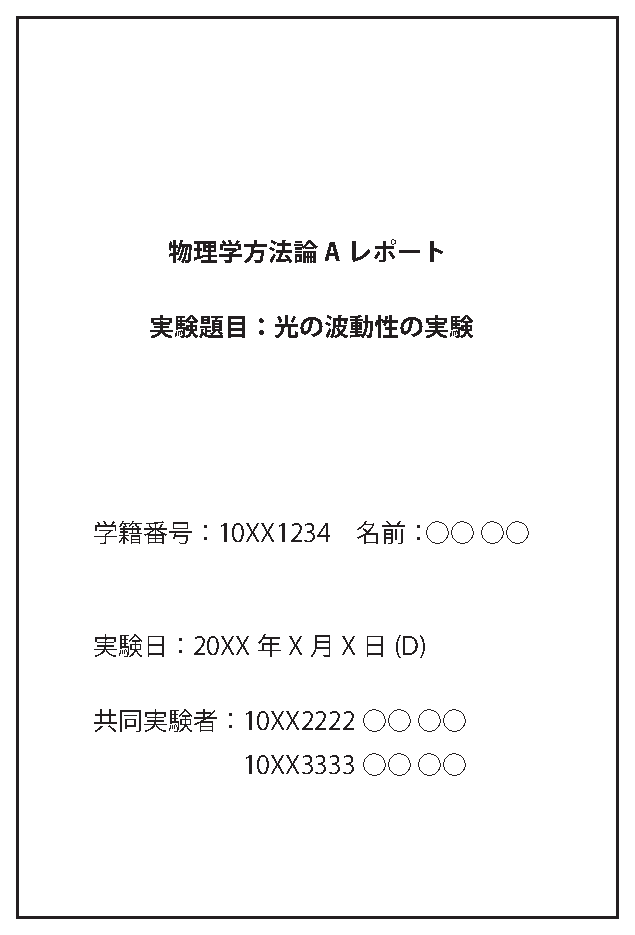
\includegraphics[scale=0.4]{00_Intro/report.eps}\\
レポートの表紙の例
\end{center}
\end{minipage}

\begin{enumerate}
\setcounter{enumi}{2}
\item レポートは、次のような順序で書くようにしましょう。

\begin{enumerate}

\item 実験の目的:
\begin{itemize}
\item 何を目的とした実験なのかを、簡潔に書くこと。
\end{itemize}

\item 実験の理論の概要

\item 実験装置、実験の手順の概要

\item 実験結果:
\begin{itemize}
\item まず、何を測定して、数値がどうであったかを書き、次に、計算の結果求められた物理量を(途中の式も含めて)書くこと。
\item 数値を書くときには、\underline{単位}を必ず記入すること。
\end{itemize}

\item 検討・考察:

\begin{itemize}
\item 実験結果の誤差について検討するなど、理論的考察を行なう。この実験から
わかったことをまとめ、実験をしてみて新たに感じた疑問があれば、そのよ
うな疑問についても調べ、考察する。
\item 調べて分かったことを記入した際には、必ず参考文献(本の題名、著者、出
版社)を最後に書いておくこと。
\end{itemize}


\end{enumerate}

\end{enumerate}


%!TEX root = ../main.tex
%
% 波の性質
%


\section{波の性質}

\subsection{「波」とは}

\subsubsection*{私たちの身の周りにある波}

\begin{center}
\begin{tabular}{ccl}
水面(海面や湖面)に立つ波 & $\Rightarrow$ & 目で形を見ることができる波\\
サイレンなどの音の波(音波) &  $\Rightarrow$ & 耳で聞くことのできる波\\
地震波 & $\Rightarrow$ & 身体で感じることができる波
\end{tabular}
\end{center}

これらは、振動が水、空気などの媒質の中を伝わっていく現象で、この振動は、
\begin{center}
\begin{tabular}{lcl}
波長 &:&$\lambda$(ラムダ)\\
振動数(周波数)&:&$\nu$(ニュー)\\
振幅&:&$A$\\
\end{tabular}
\end{center}
によって表わされます。この場合の波の伝わる速度$v$は、
\begin{center}
波の伝わる速度:$v=\lambda \nu$
\end{center}
です。また、振動数(周波数)と「波が1波長進むのにかかる時間」=周期とは互いに逆数の関係があり、
\begin{center}
周期:$T=\frac{1}{\nu}$
\end{center}
となります。
\begin{center}
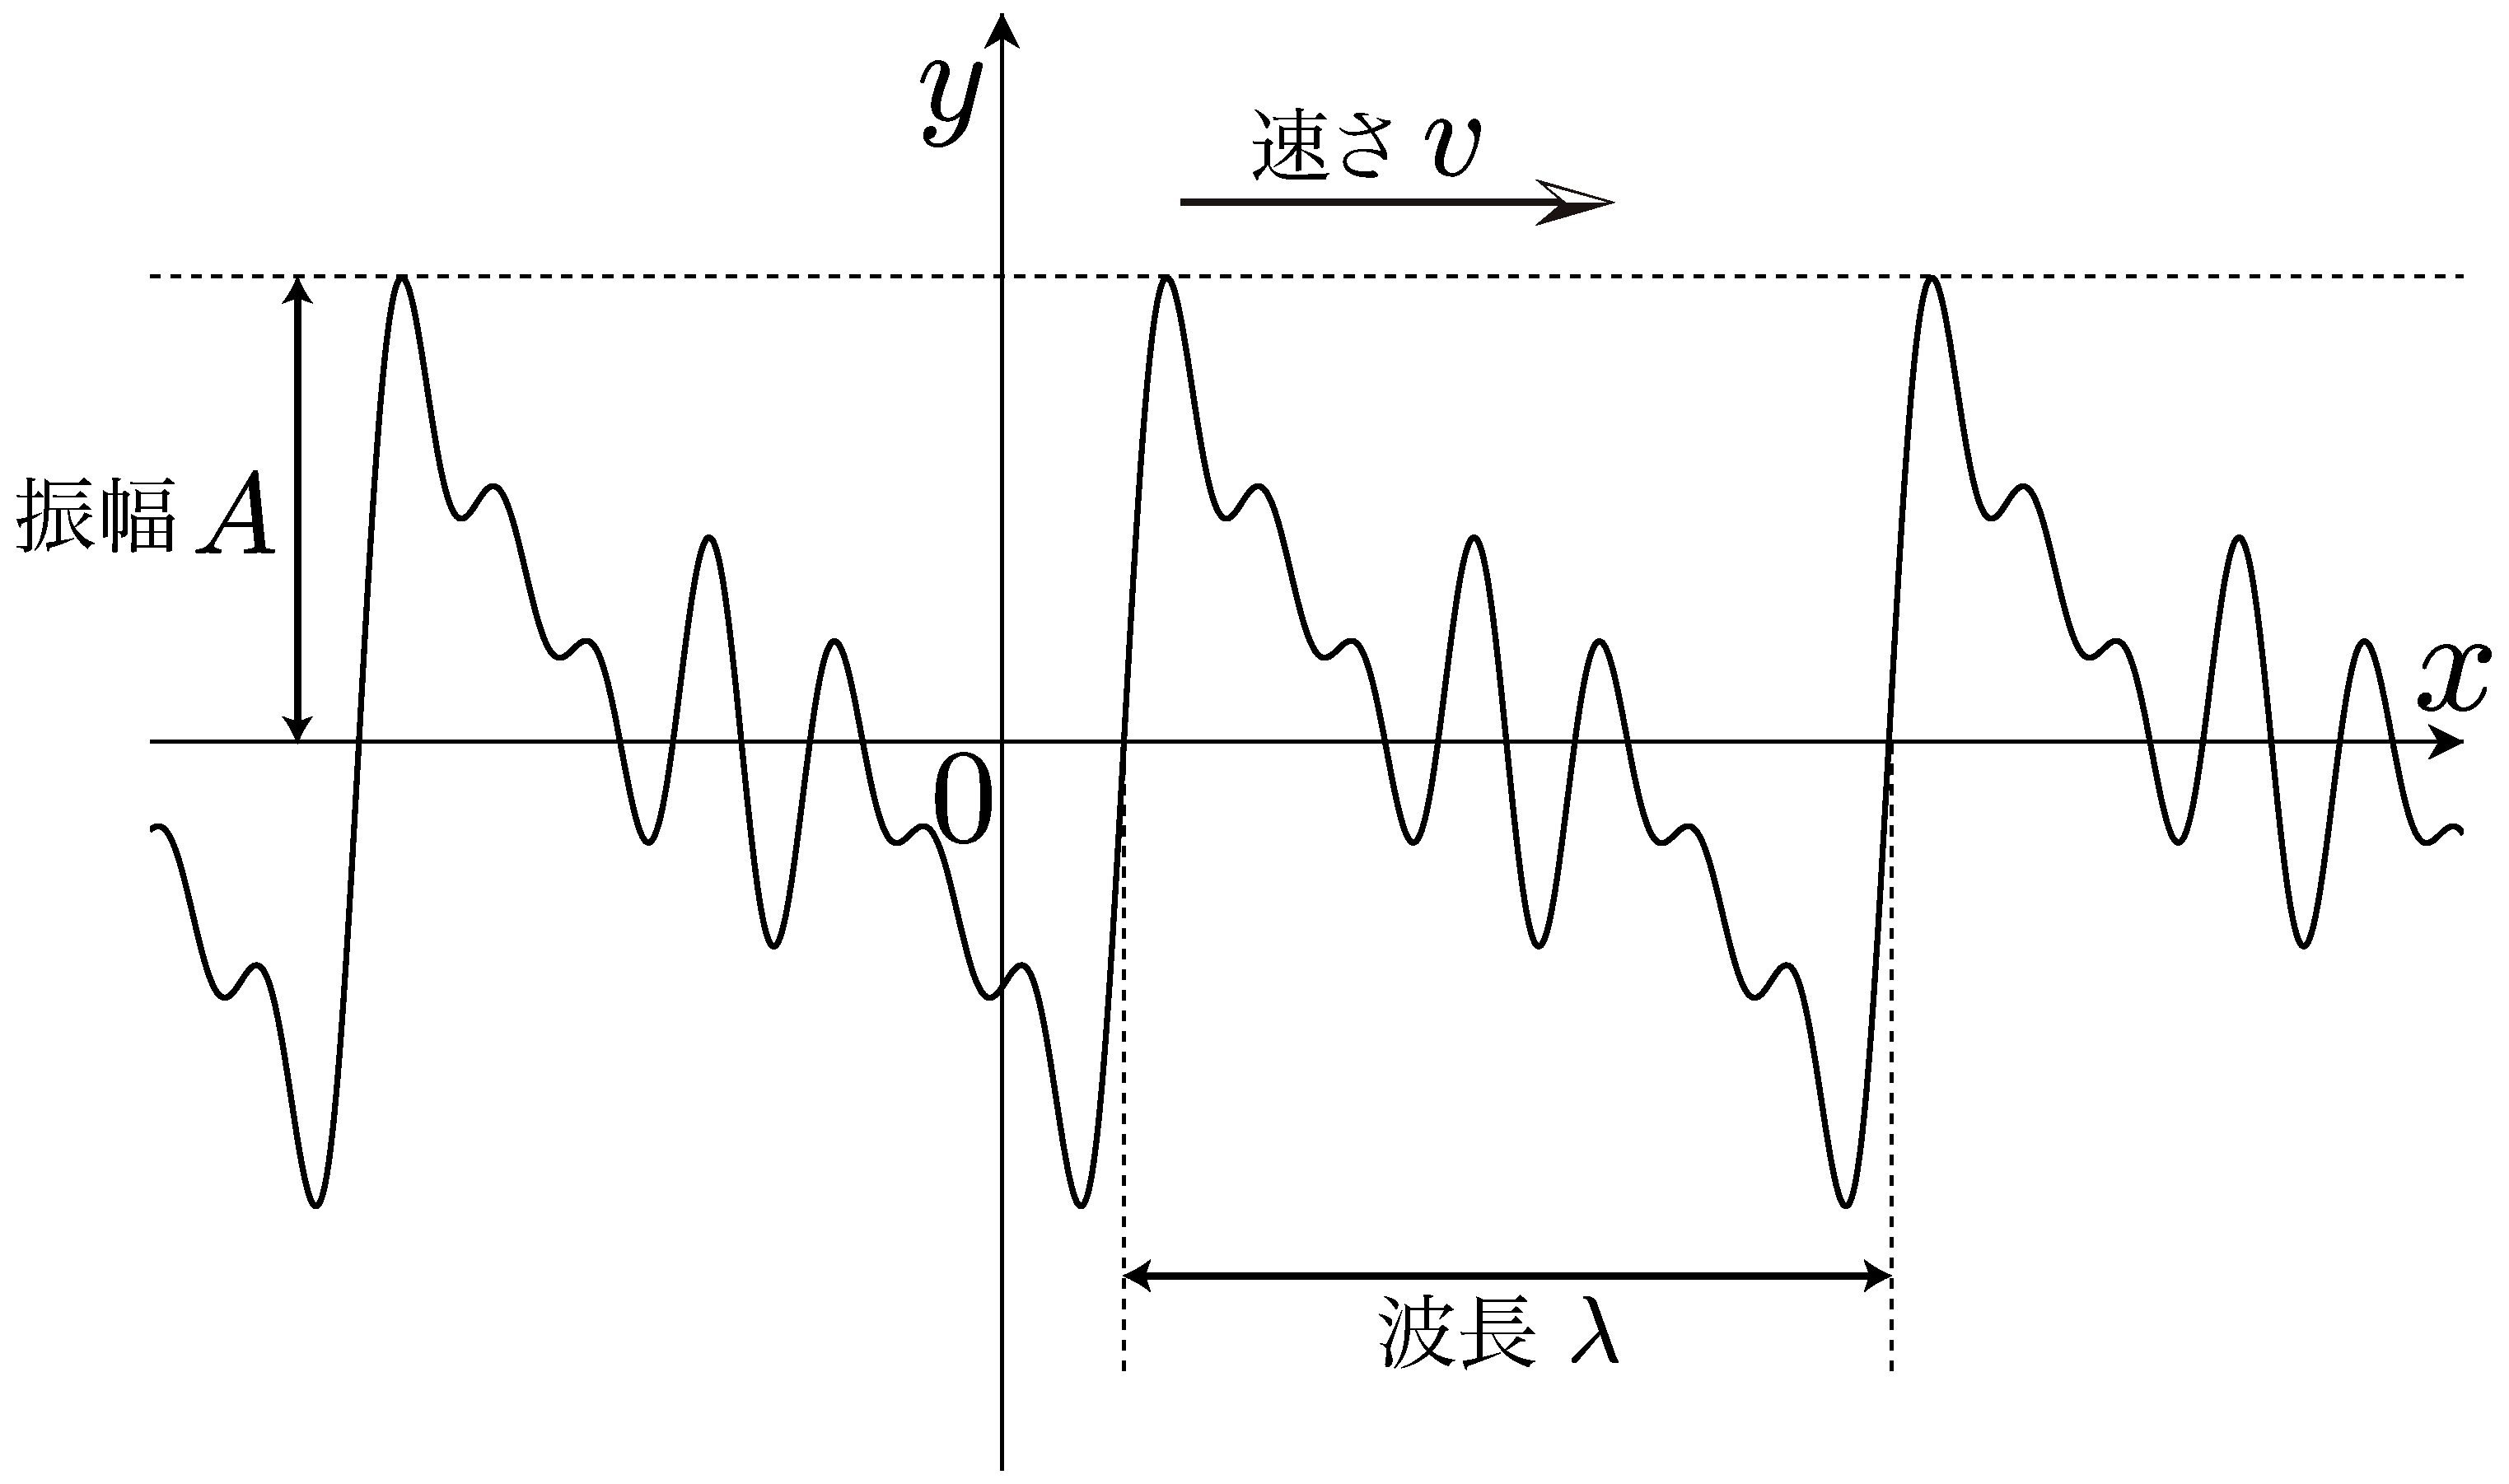
\includegraphics[scale=0.18]{01_Wave/wave1.eps}
\end{center}

波の基本の形は次のような正弦波(サイン関数で表わされる波)で、変位$y$は、時間$t$と位置$x$の関数で表わされます。
\[
y = A \sin\left(2\pi \left(\frac{t}{T}-\frac{x}{\lambda}\right)\right)
\]
ここで、式中の$\pi$は円周率=$3.1415\ldots$です。
\begin{center}
\begin{tabular}{ccc}
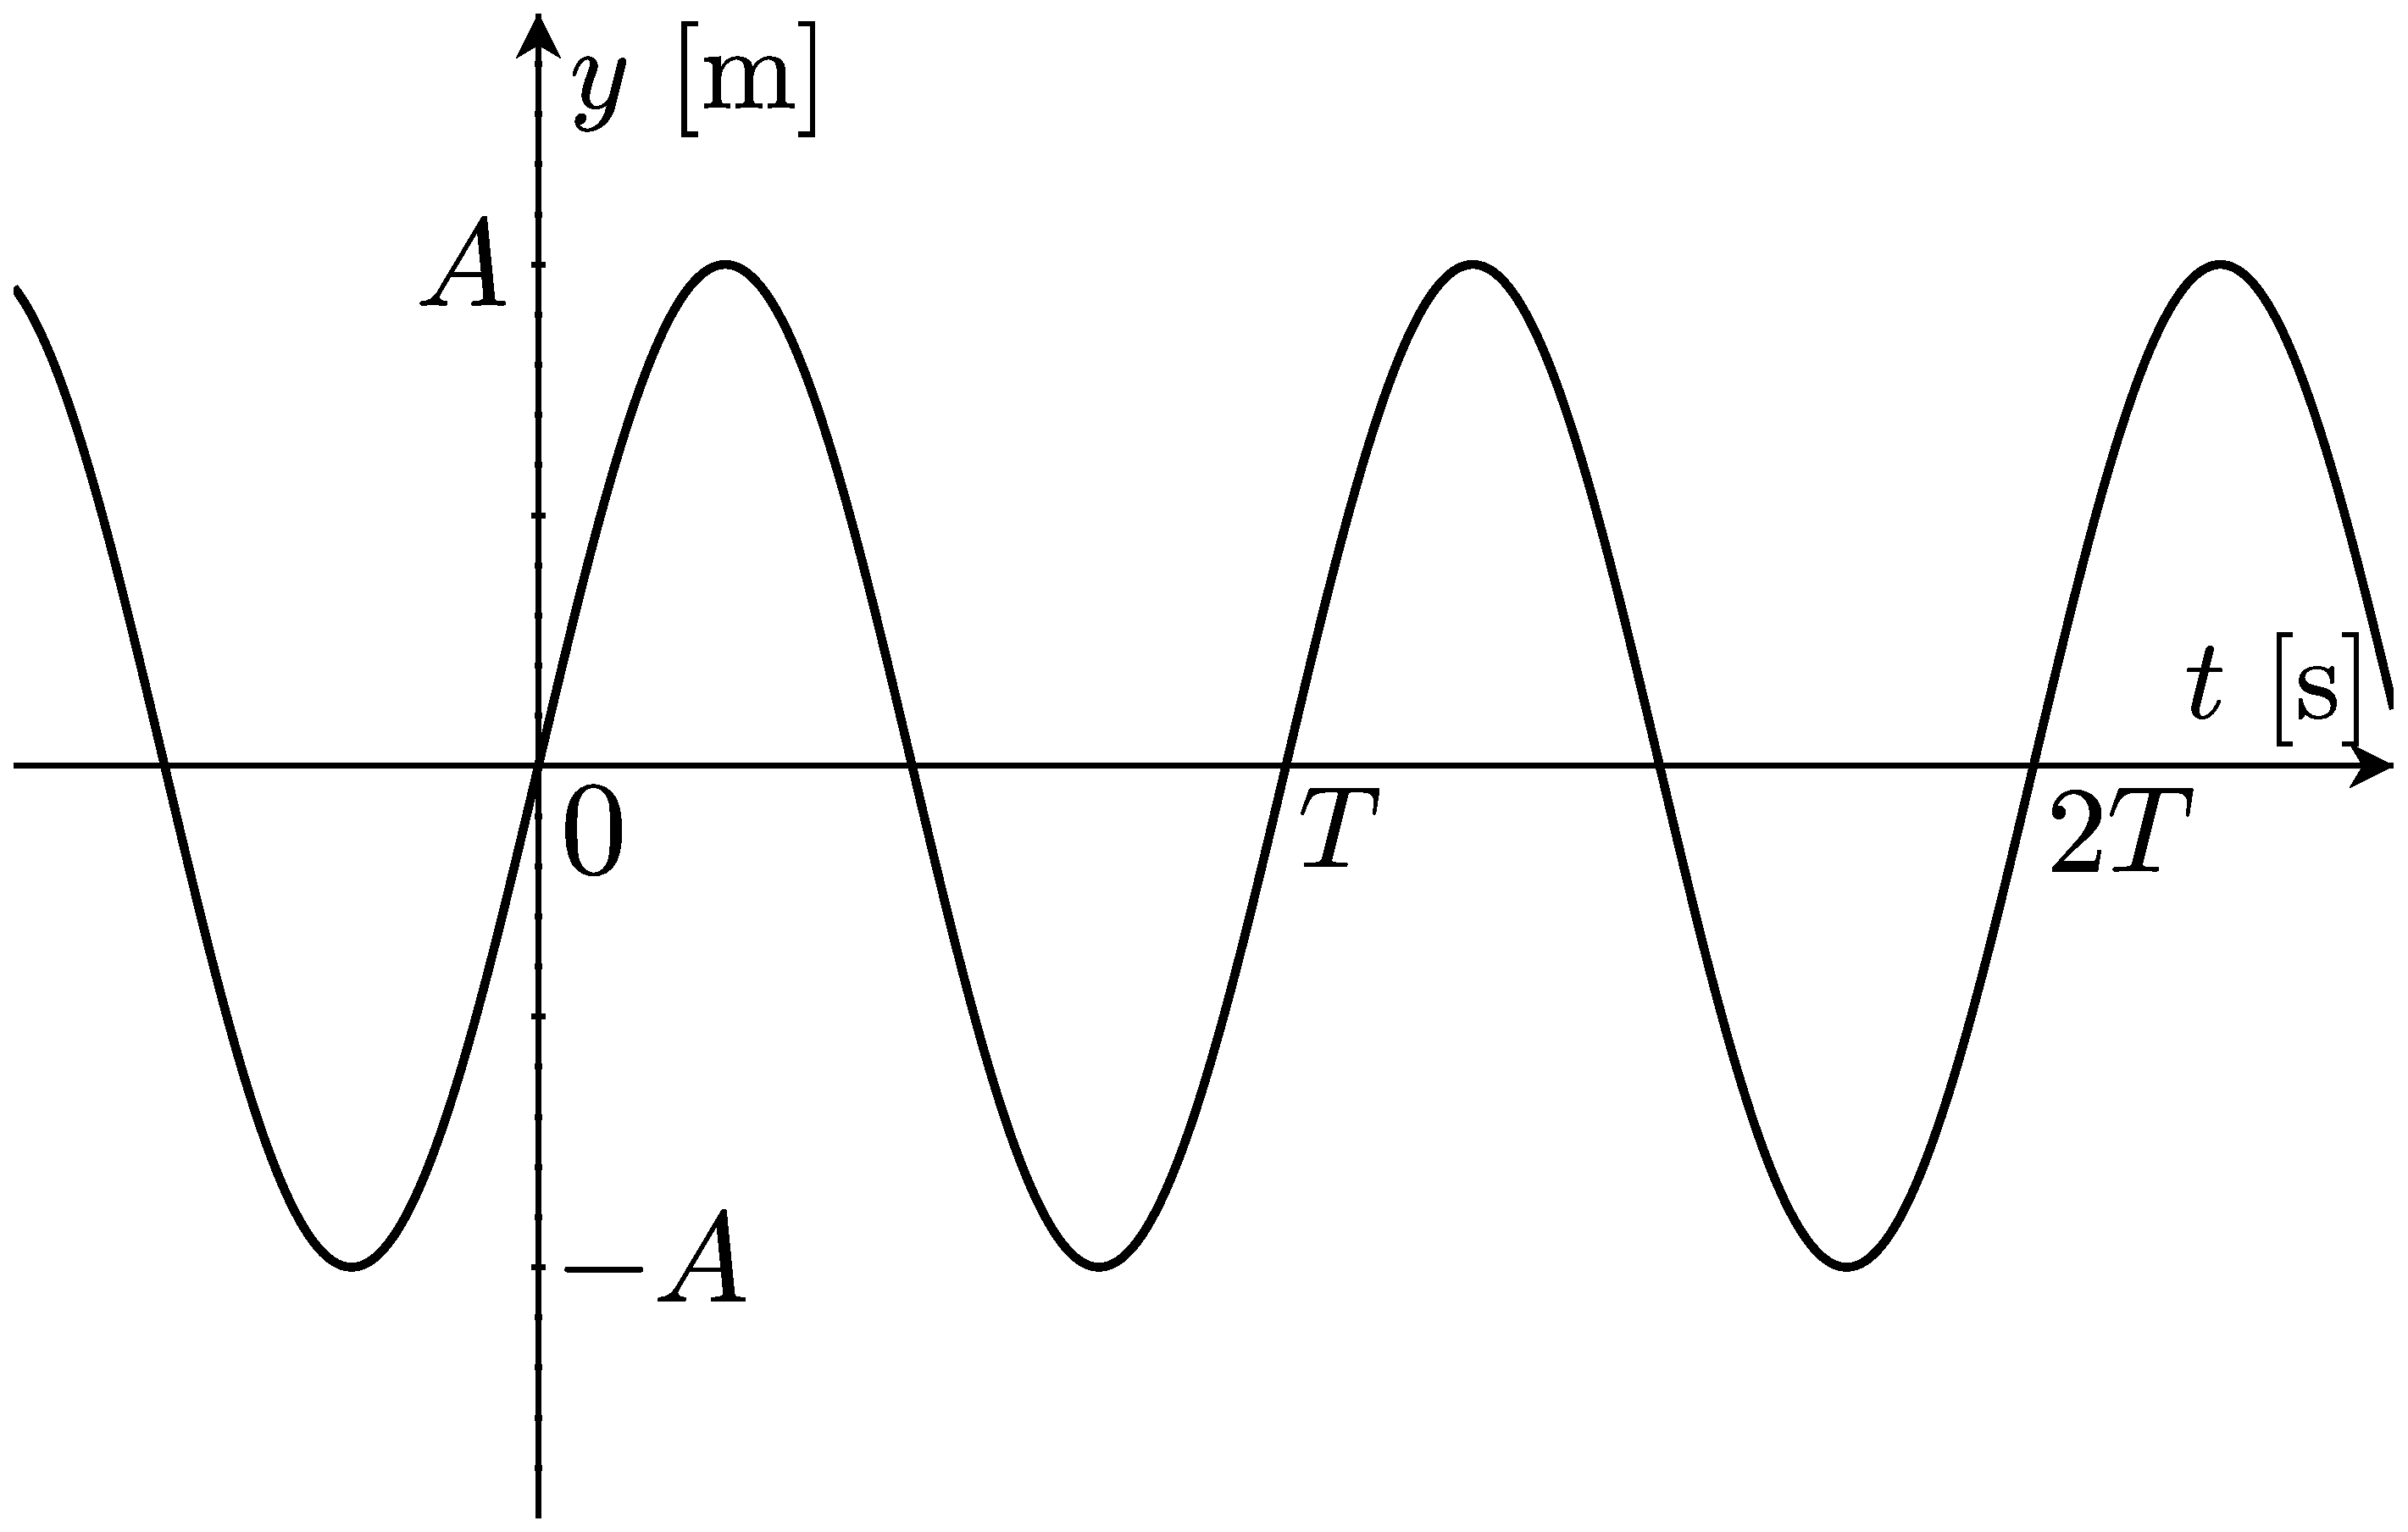
\includegraphics[scale=0.14]{01_Wave/wave2.eps}&&
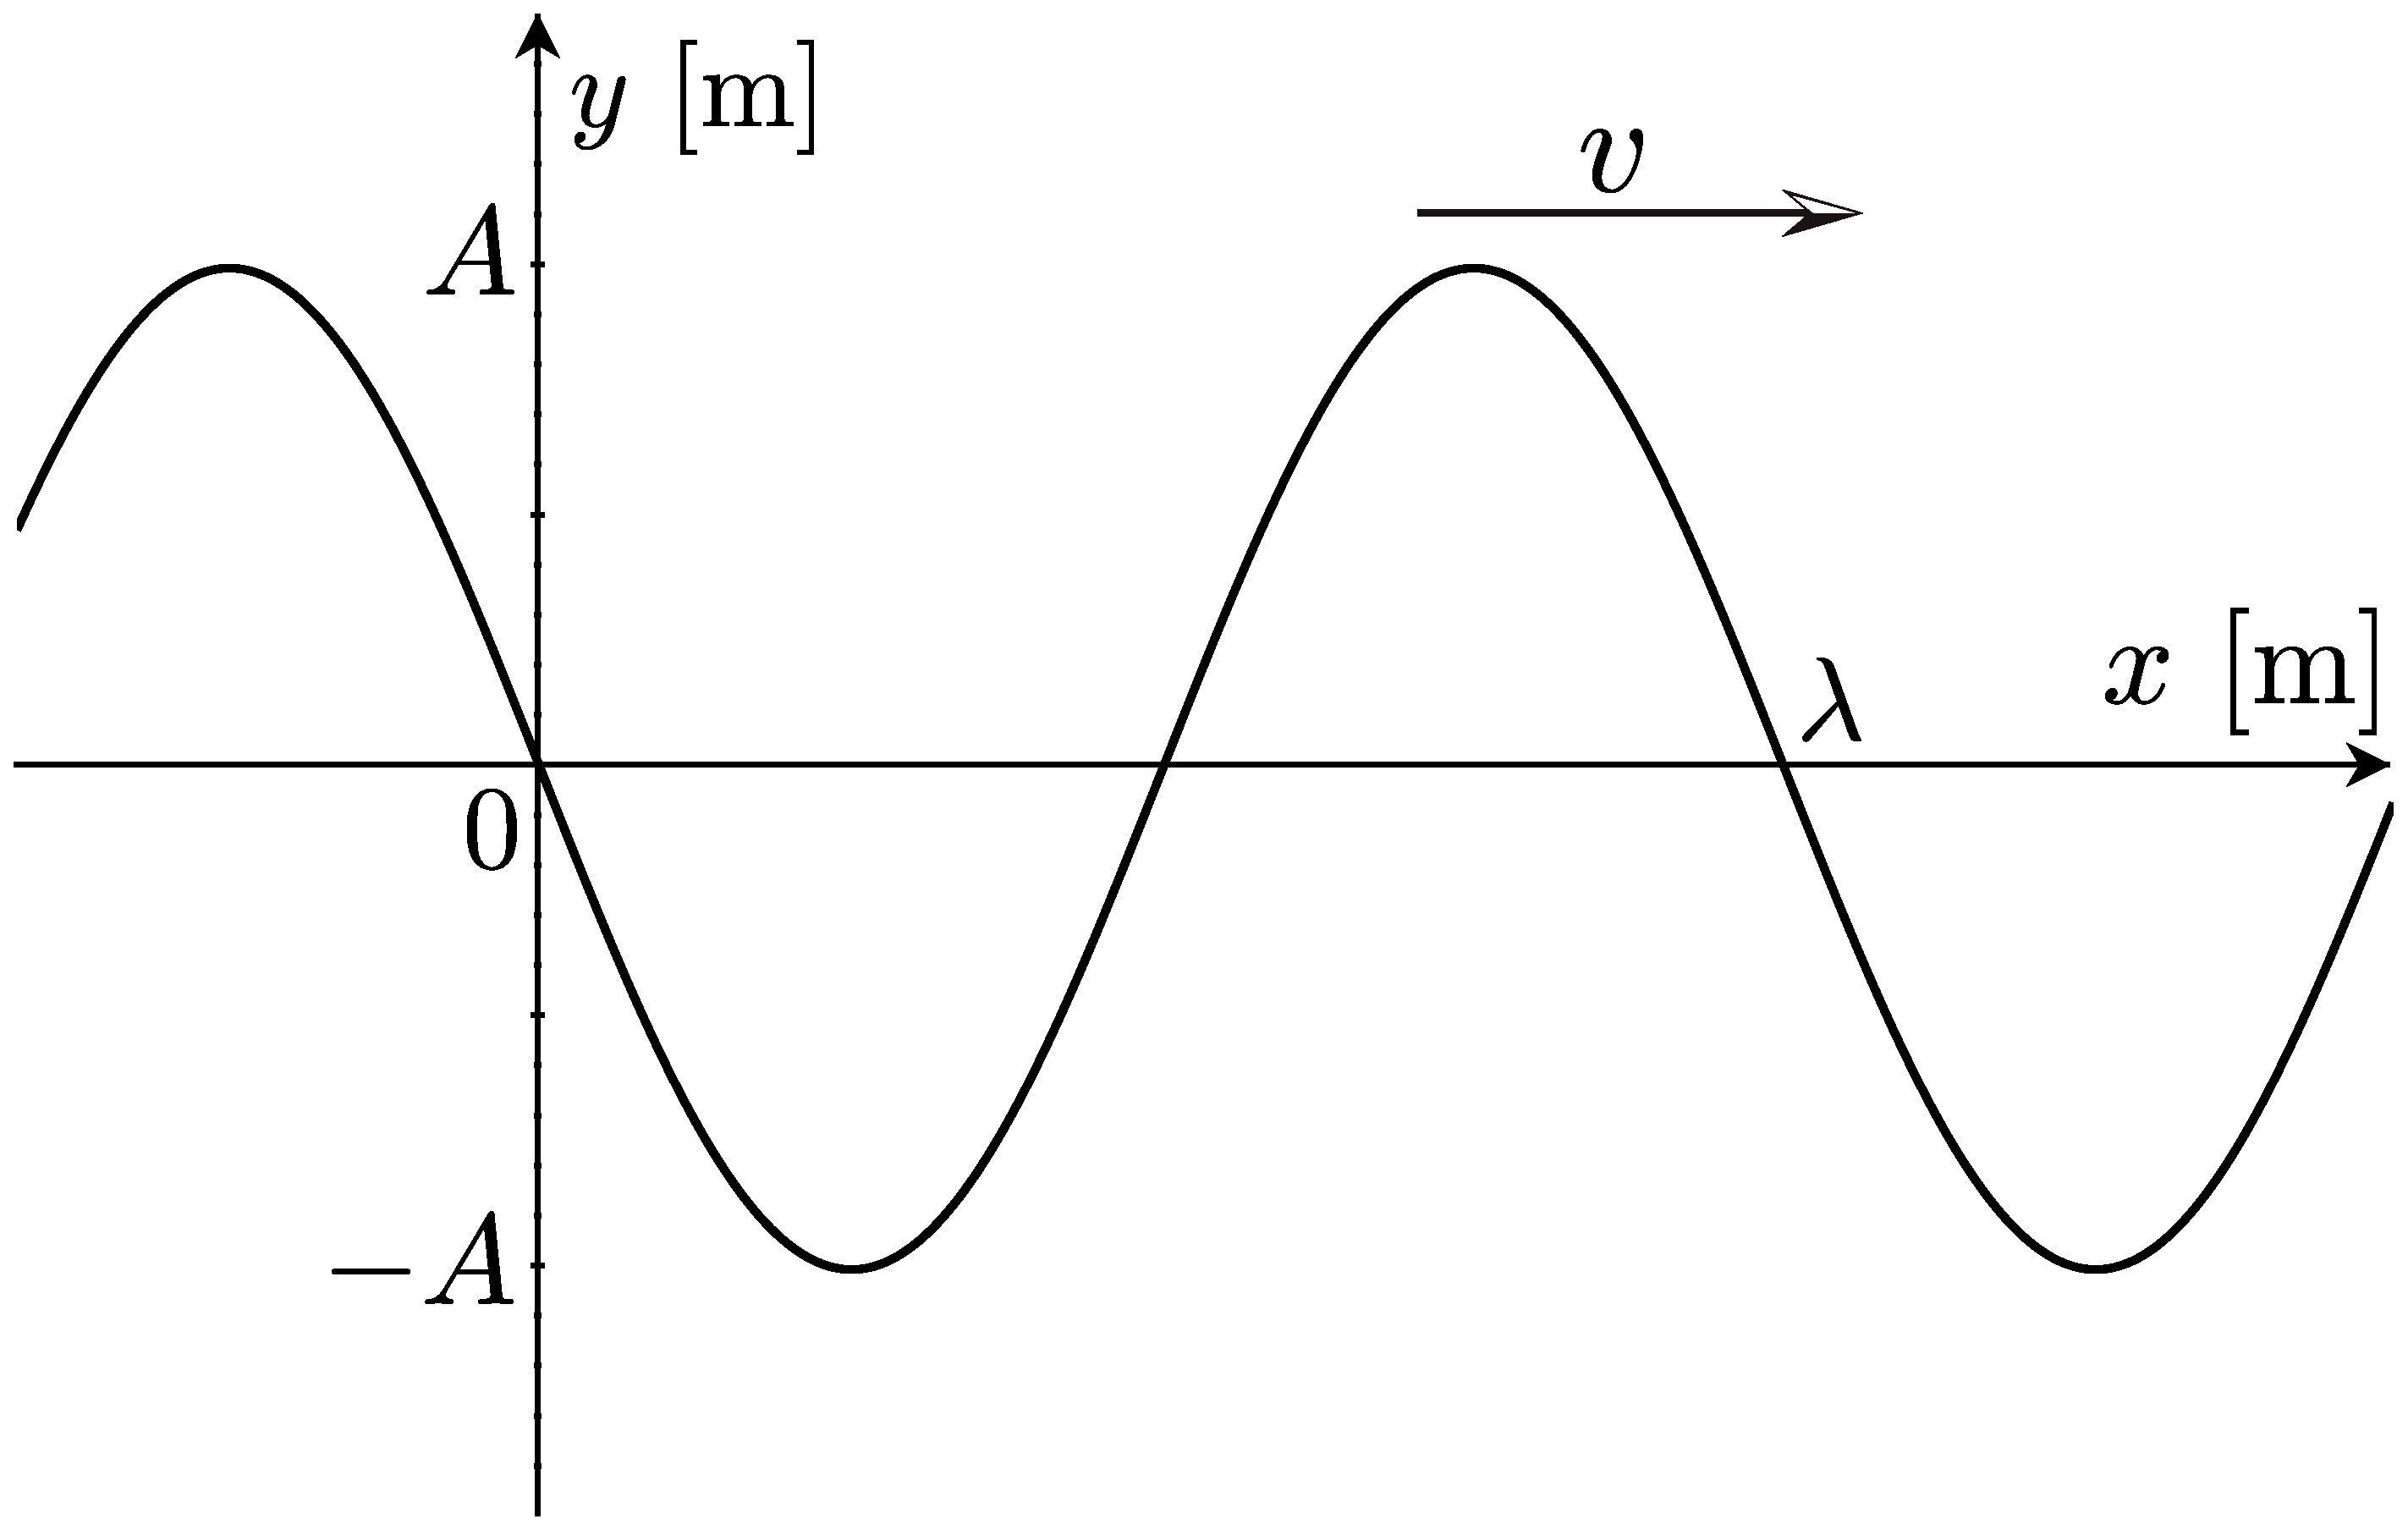
\includegraphics[scale=0.14]{01_Wave/wave3.eps}\\
(a) $x=0$の点の振動のグラフ && (b) $t=0$のときの波のグラフ\\
\end{tabular}
\end{center}



%\subsubsection*{波の性質と種類}

\begin{itemize}

\item 波には、{\bf 屈折}、{\bf 反射}、{\bf 回折}、{\bf 干渉}などの性質があります。

\item 波の振動の伝わり方によって種類が分けられています。
\begin{center}
\begin{tabular}{rcl}
{\bf 横波} &$\cdots$& 波の振動方向が、波の進行方向に対して垂直のもの\\
&& 例)水面の波、地震のS波\\
{\bf 縦波} & $\cdots$ &波の振動方向が、波の進行方向と同じもの\\
&& 例)音波、地震のP波
\end{tabular}
\end{center}

\end{itemize}


\subsection{波の干渉と回折}

\subsubsection{波の位相と干渉}


波の1周期における波形の位置のことを位相といい、1周期を360度=$2\pi$として角度で 
表します。すなわち、波の基本形の式
$y=A\sin\left(2\pi\left(\frac{t}{T}-\frac{x}{\lambda}\right)\right)$
において、 
$
2\pi\left(\frac{t}{T}-\frac{x}{\lambda}\right)
$
が位相で、 
$
\frac{t}{T}
$
は時間という物差しで時間$t$の中に波がいくつ入るかを、
$\frac{x}{\lambda}$は長さで見て距離$x$の中に波がいくつ入るかを数えています。

波の重ね合わせの原理により、同位置同時刻において位相が同じである2つの波は強め合い、位相がちょうど「半周期分=180度」ずれている波は弱め合います。
このような波の性質を{\bf 干渉}といいます。

\begin{center}
\begin{tabular}{ccc}
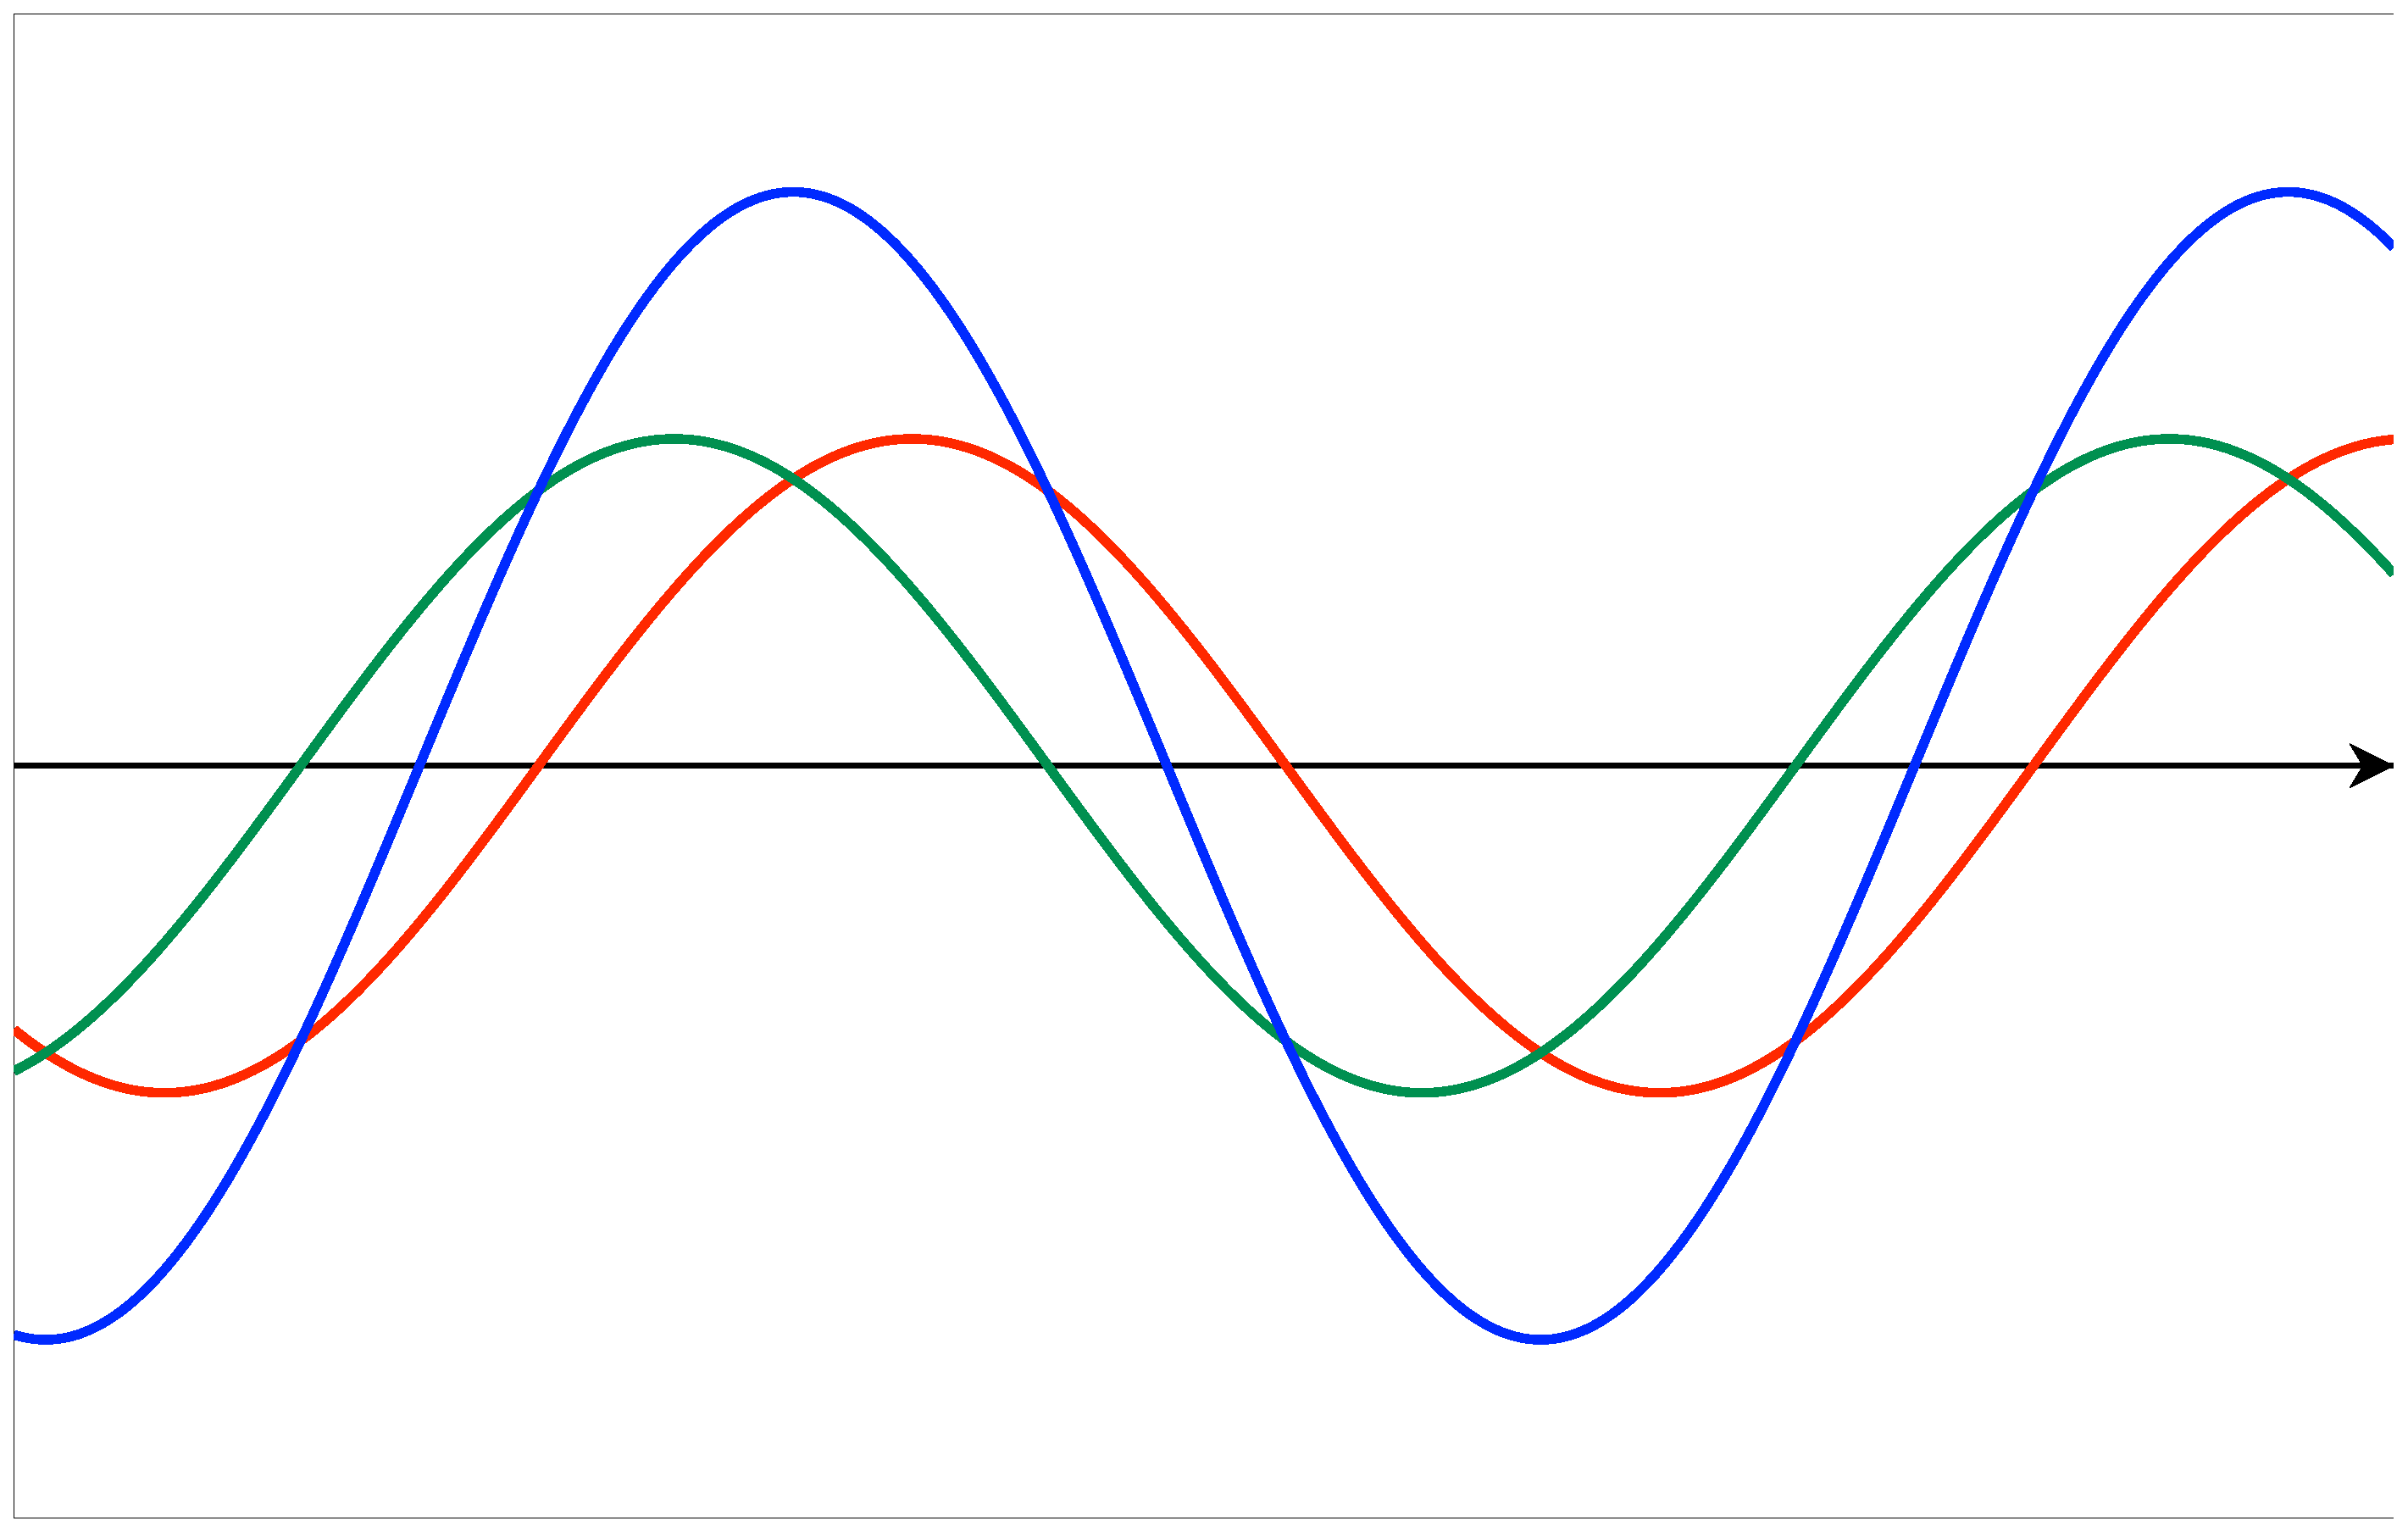
\includegraphics[scale=0.1]{01_Wave/interference1.eps}&
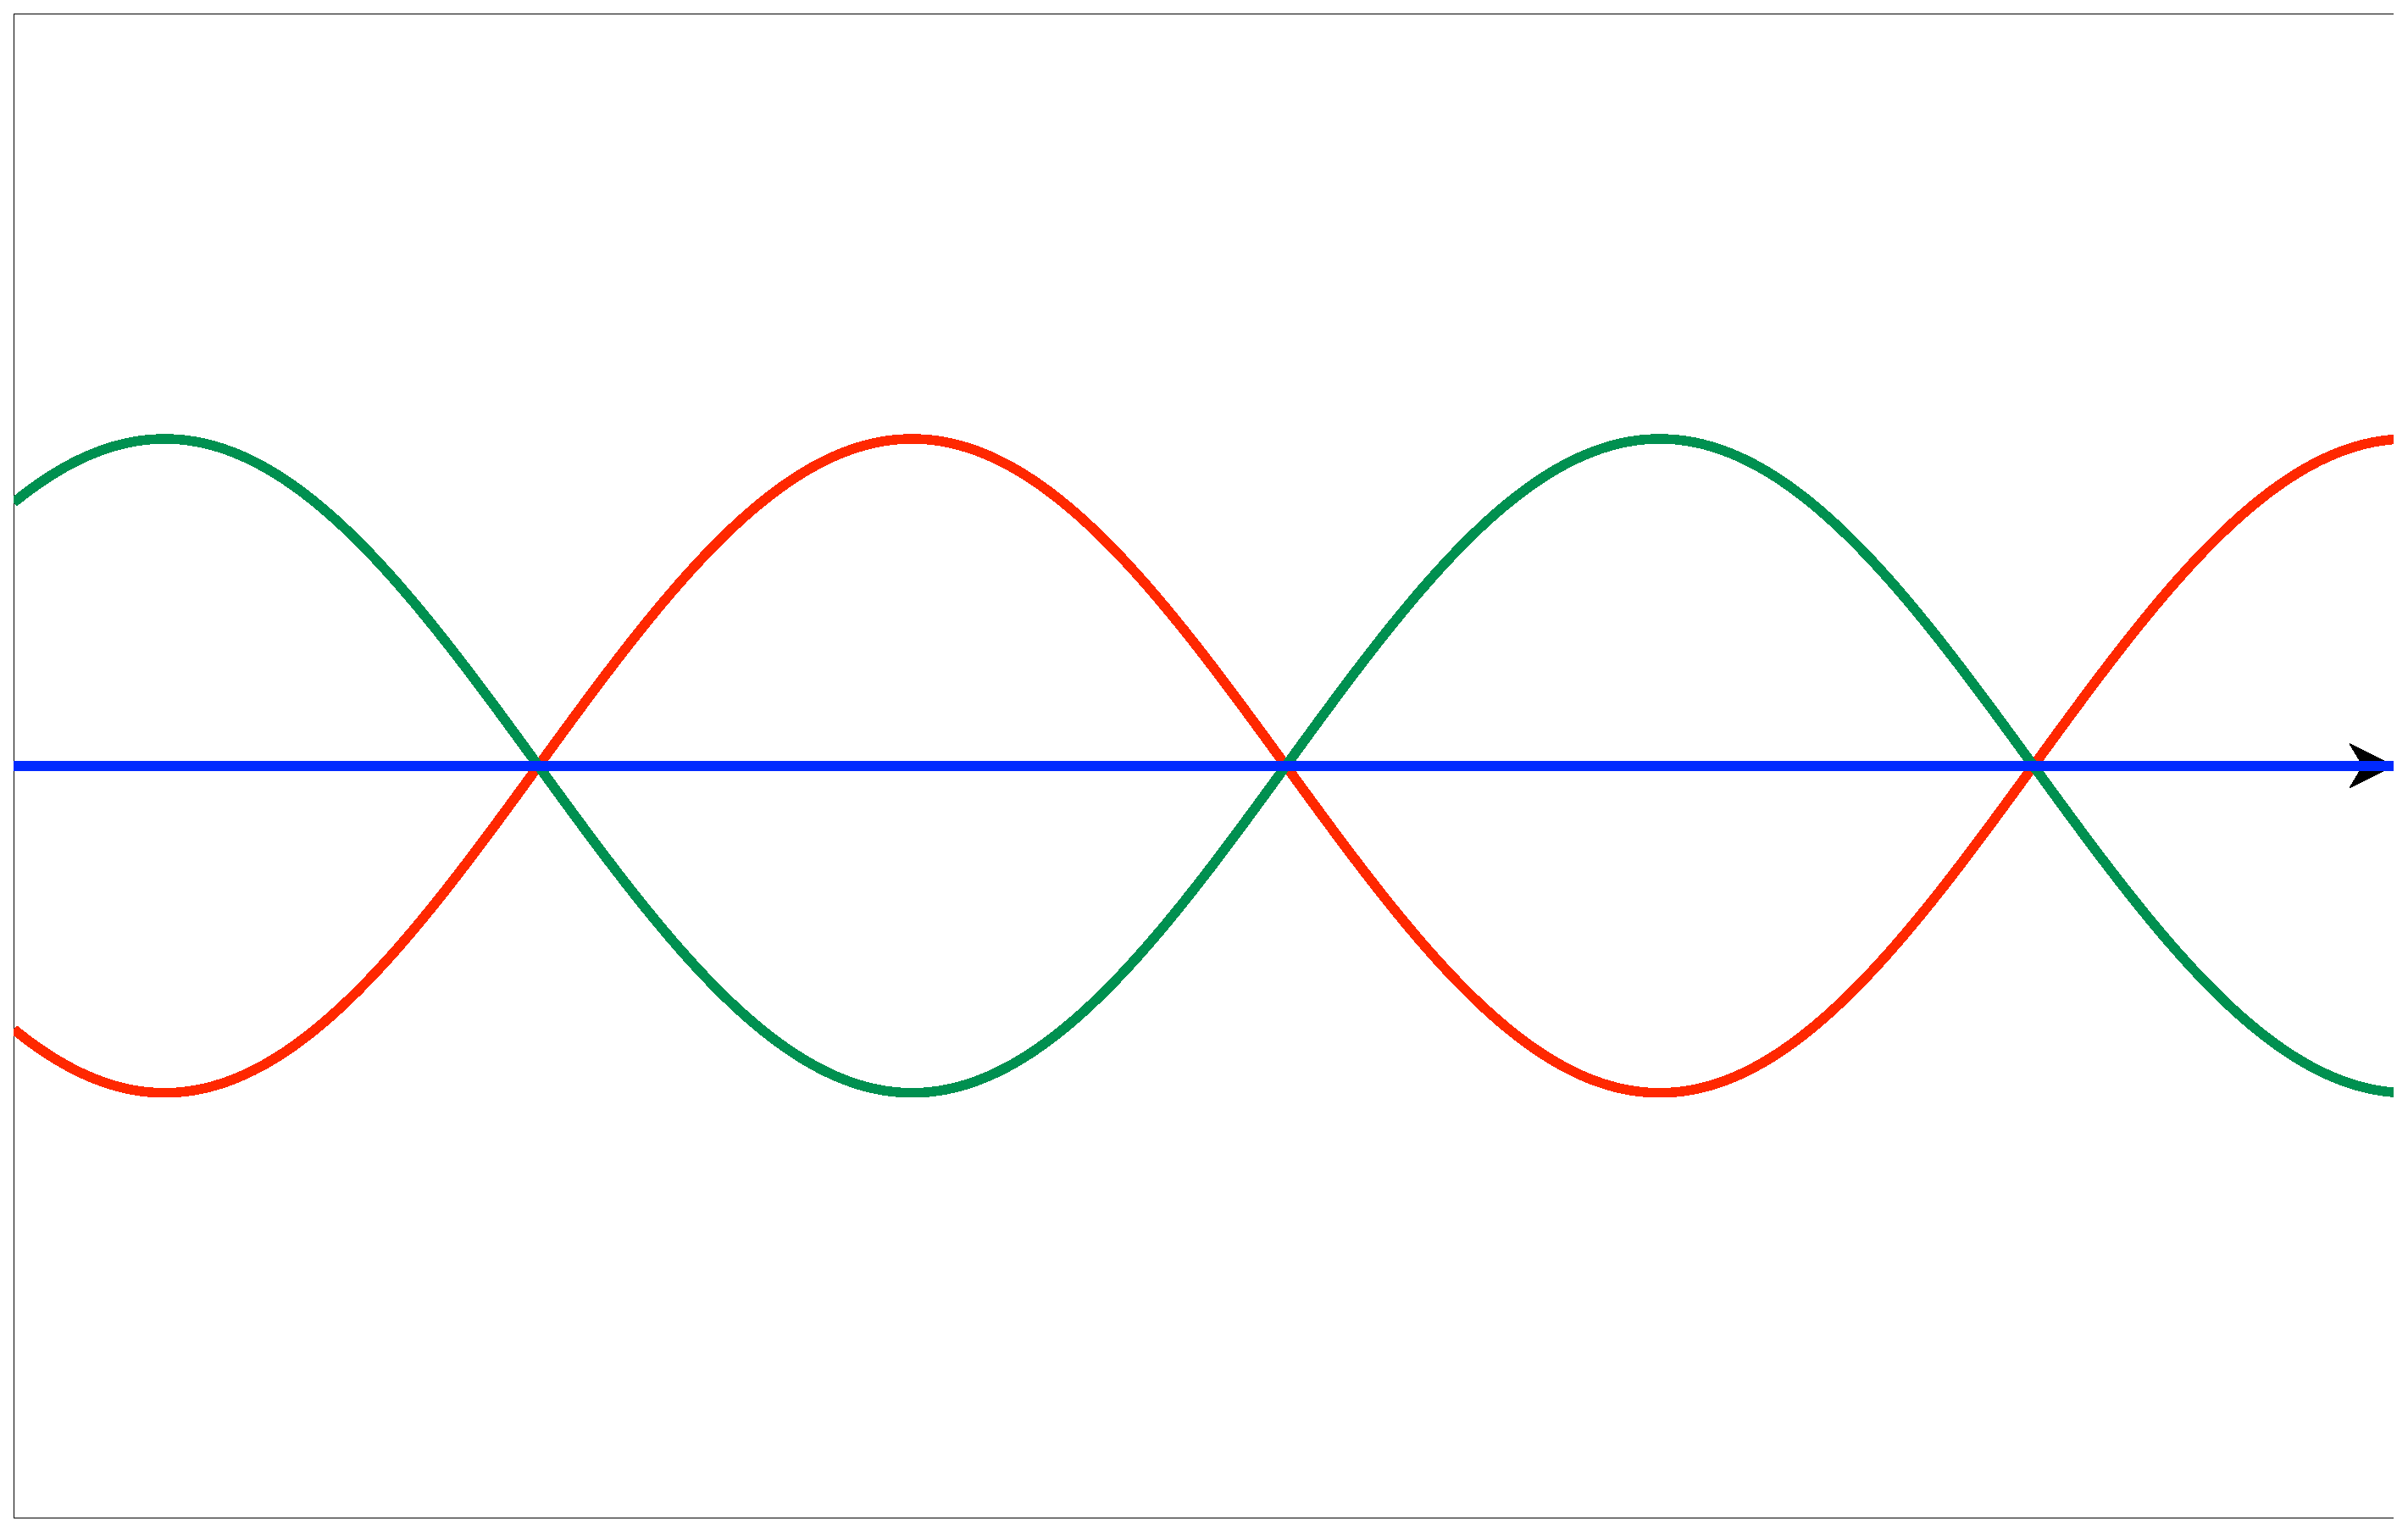
\includegraphics[scale=0.1]{01_Wave/interference2.eps}&
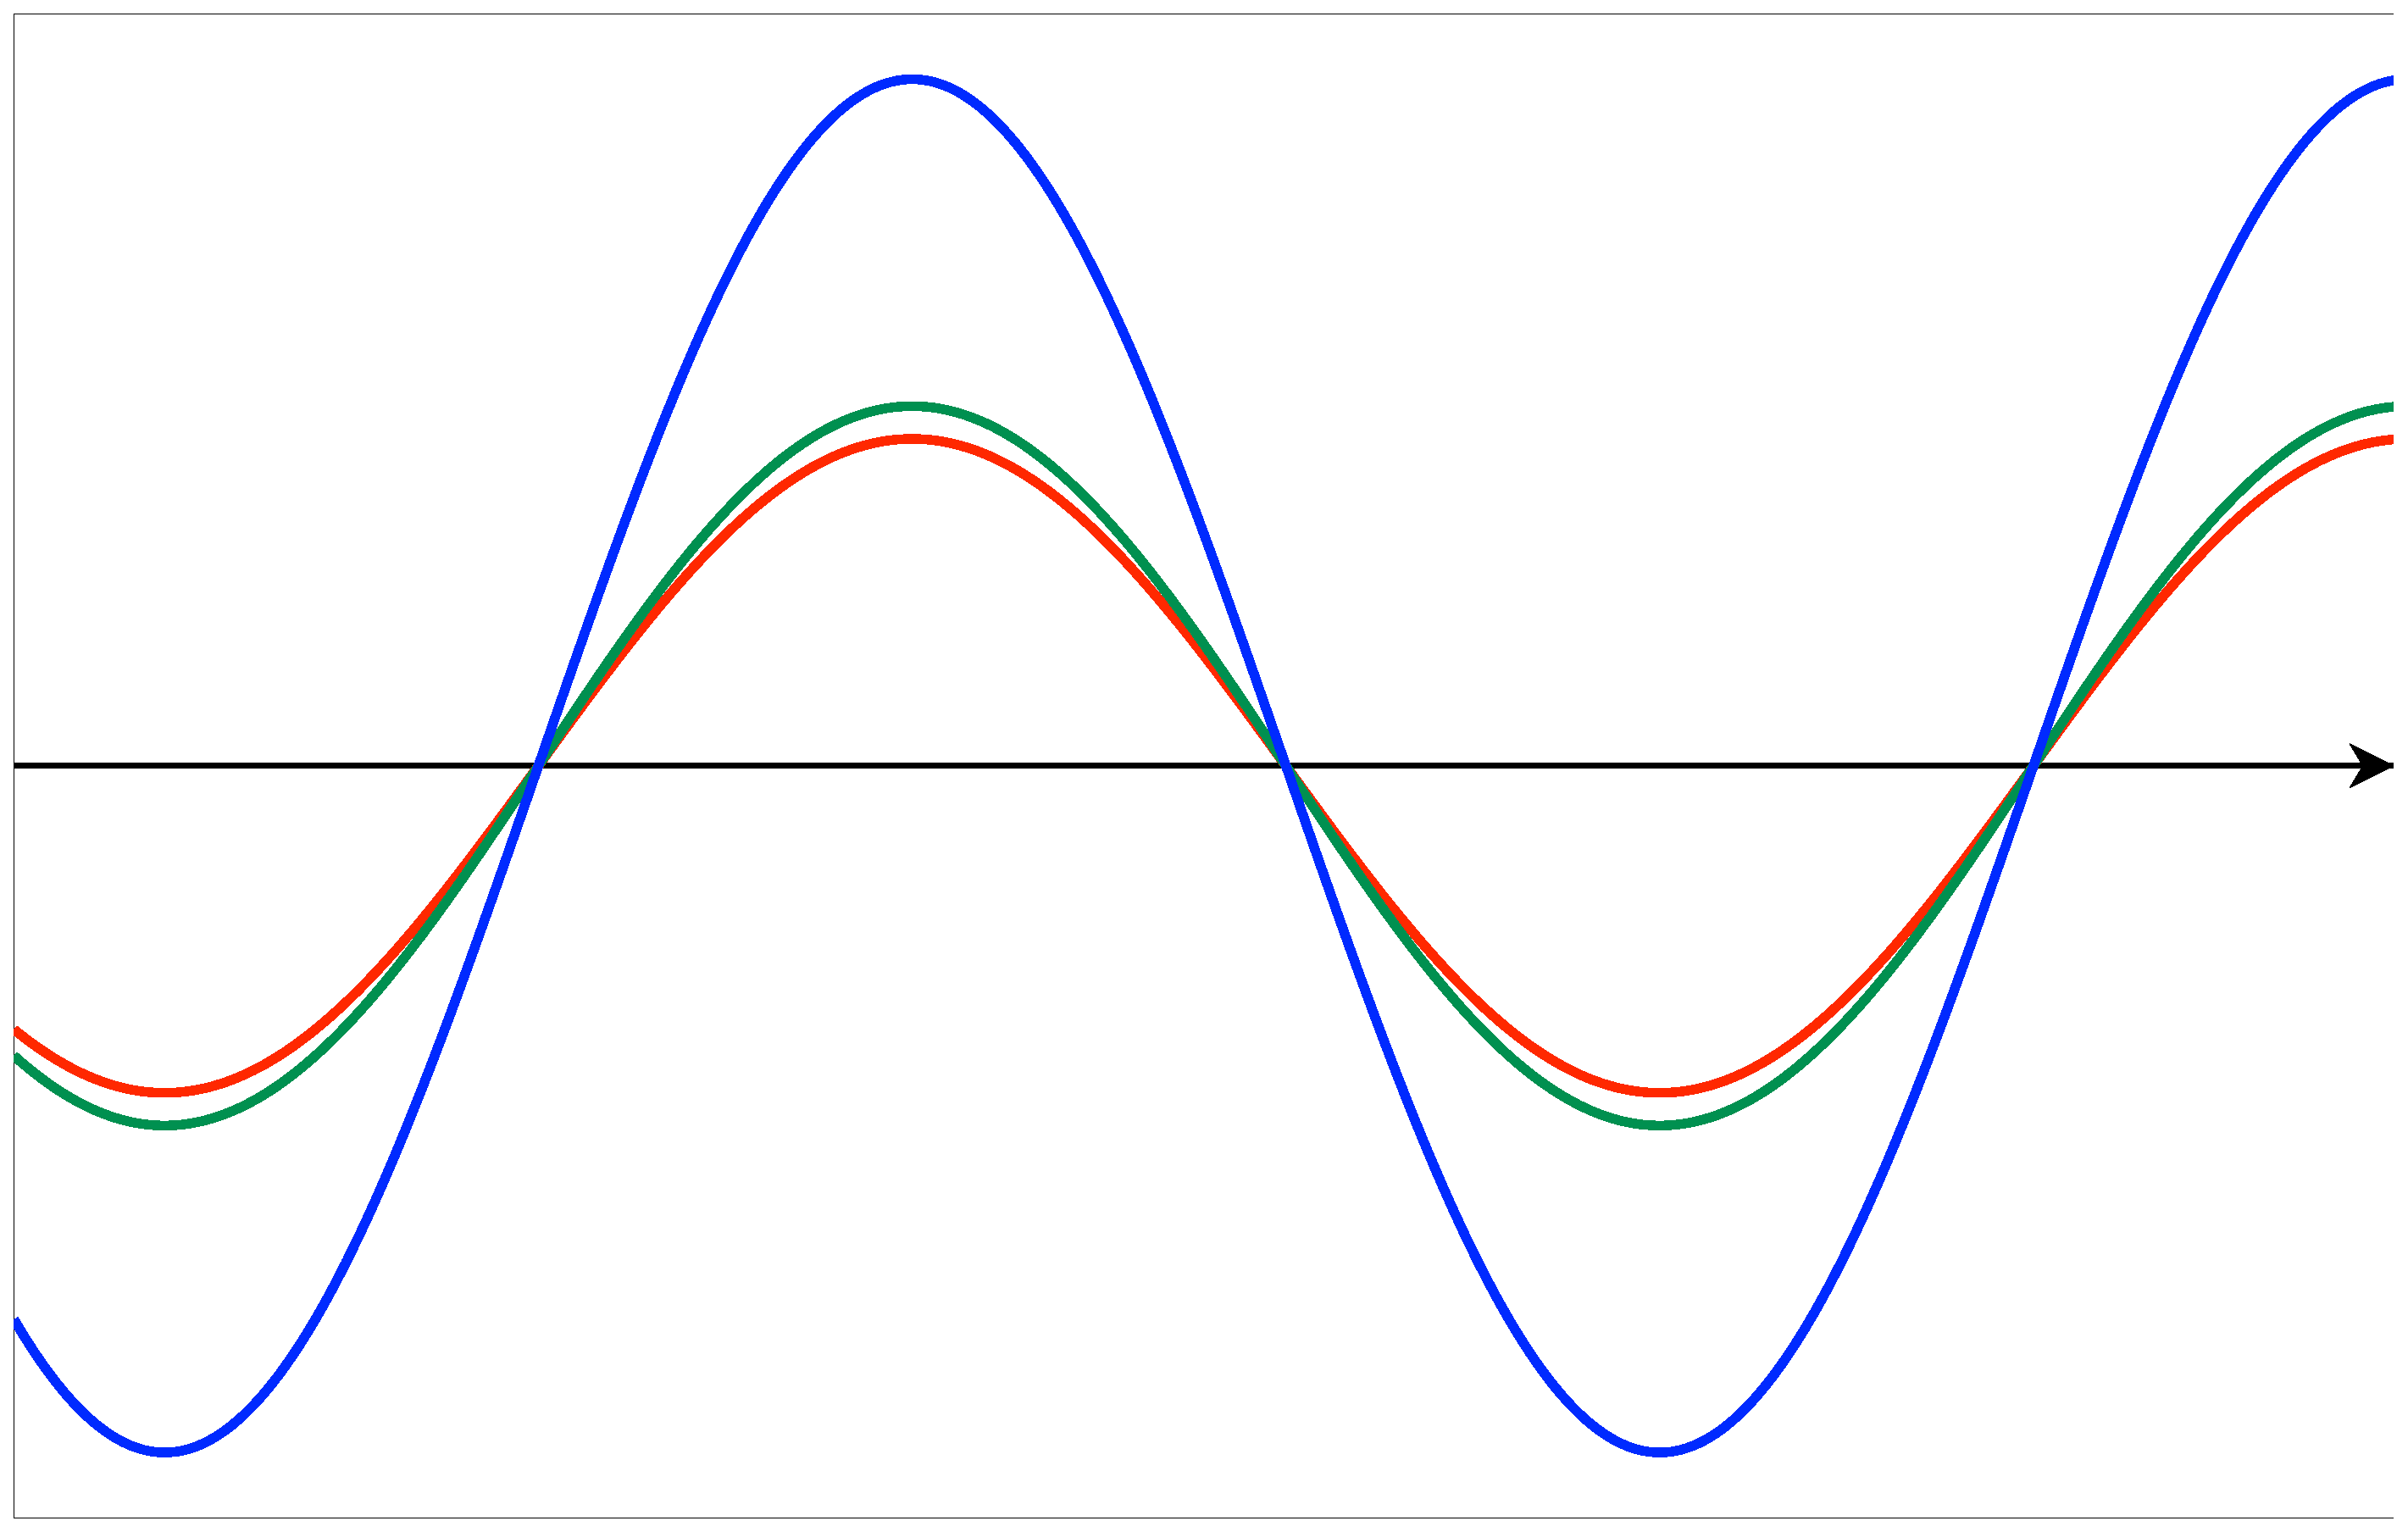
\includegraphics[scale=0.1]{01_Wave/interference3.eps}\\
(A) 強くなる
& (B) 打ち消し合う
& (C) 最も強め合う\\
& (山と谷が合致) & (山と山、谷と谷が合致)
\end{tabular}\\
\bigskip
波の干渉:{\color{red}\maru{1}}+{\color{green}\maru{2}}$\rightarrow${\color{blue}\maru{3}}
\qquad
{\color{red}\maru{1}}の波と{\color{green}\maru{2}}の波が干渉して{\color{blue}\maru{3}}の波ができる
\end{center}

\subsubsection{波の回折}

\begin{wrapfigure}[6]{r}{5.5cm}
\vspace*{-0.8cm}
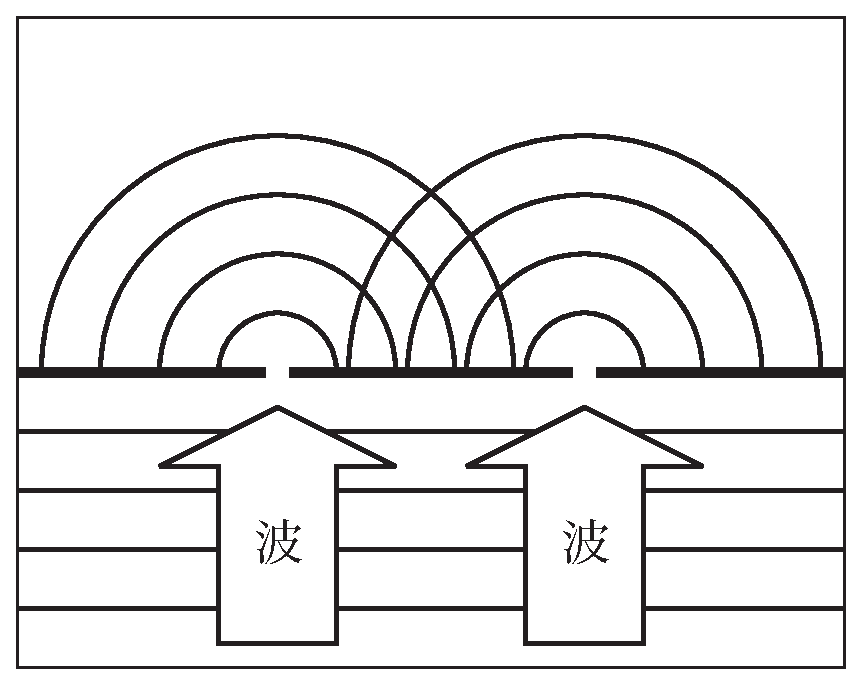
\includegraphics[scale=0.38]{01_Wave/diffraction.eps}
\end{wrapfigure}

進行している波を細いスリットの開いた障壁で遮ると、スリットを通っ
た波は直進せず、スリット上の各点を中心とした球面波を発生し、障壁の裏側まで回り込むよ 
うに伝わります。この現象を波の{\bf 回折}といいます。
スリットの幅に比べて波の波長が大きいほど、回折の程度は大きくなります。
($\Leftrightarrow$波長と比べてスリットの幅がかなり大きければ、回折は起こらず波は直進します。)

\subsection{ドップラー効果と衝撃波}

波が発生している場所(波源)が移動しているとき、進行方向の前方の波長は短く詰まり周波数が高くなり、
後方の波長は長く伸び周波数は低くなります。
この現象のことを{\bf ドップラー効果}と言います。

静止している観測者に向かって伝播速度$V$、振動数$\nu$の波の波源が速度$v$で同一直線上を移動しているとき、
観測者が受ける波の振動数$\nu'$は
\[
\nu' = \nu \times \frac{V}{V-v}
\]
となります。ただし、$v$は観測者に向かう向きを正とし、遠ざかるときは負とします。

この式を見ると、波源の移動速度が波の伝播速度$V$と等しくなったとき、波源の移動方向前方
の波は圧縮され振動数は無限大になります。このとき波源の先頭で重なりあった強い波を{\bf 衝撃波}
と言います。一般に波源の移動速度が波の伝播速度を上回ったとき衝撃波が発生します。

音速を超えて飛行するジェット機などの周囲にも衝撃波が発生し、
その衝撃波が大音響として聞こえることもあります。

\subsection{水深と波の速度}

水面で発生する波の場合、その波の高さや水深によって波の進行速度が変わります。波の高さを$h$、水深を$d$、
重力加速度を$g(=9.8\, [{\rm m/s}^2])$とすると、水波の進行速度は近似的に
\[
v = \sqrt{g(h+d)}
\]
で与えられます。この式から、水深の深い海の中心部よりも水深の浅い沿岸部の方が波の速度が遅くなる
ということがわかります。

\newpage

\jikken

\begin{itemsquarebox}[c]{\bf 実験用具}
水波投影装置、水波発生器(空圧式)、水波発生装置(磁石式)、アクリルブロック、消しゴム、カメラ機能付きスマートフォン(デジタルカメラ)
\end{itemsquarebox}

\bigskip

\subjikken{水波の観察}

\begin{enumerate}

\item 水槽に水を張り、ランプを点灯させます。

\item 水波発生器(空圧式)に単波用ノズル(L字型)を取り付けます。

\item 水波発生器(空圧式)のスイッチを入れ、ノズルの先端を水面に近づけ噴射量の調整をします。

\item ランプの光の角度等を水波が観察しやすいように調節します。

\item アクリルブロックや消しゴム等でスリットを作り、水波がスリットを通ったときの波の回折の様子を観察しましょう。水波はスマートフォン等でスロー動画撮影して記録すると観察が容易になり、水波の伝わる様子がよくわかります。

\item ノズルの先と水面との距離を一定に保ち、波源を一方向に動かします。
そのときの水波の様子をスマートフォン等で撮影し、観察します。波源の進行方向と
その反対側で水波の形状(波長)はどうなっているでしょうか? $\Rightarrow$ドップラー効果

\item 波源の移動速度をさらに速くし、水波の速度を超えると水波の形状はどうなるでしょうか? $\Rightarrow$衝撃波面の形成

\item 水波発生装置(磁石式)を水槽の縁に取り付け、振動片先端が水面に接するようにします。

\item 水波発生装置(磁石式)のスイッチを入れ、ダイアルで振動周波数の調整をします。
(ダイアルを最大にしてから始動させます。)

\item 2つの波源から出た水波が強め合ったり、弱め合ったりする時の水波の形状を観察します。 $\Rightarrow$波の干渉

%\item バットにプラスチック板を斜めにして沈め、そこにぶつかった水波の様子を観察しましょう。
%水深と波長の間に何か関係があるでしょうか? また、その関係から何がわかるでしょうか?

\end{enumerate}

%※ デジタルカメラはストラップなどを手に巻き付けるなどしてしっかり固定し、水を入れたバットに落としたりしないよう注意して操作しましょう。



%!TEX root = ../main.tex
%
% 波の性質
%


\section{気柱の固有振動と音速の測定}

\subsection{気柱の固有振動}

瓶の口に唇をあて、息を吹きかけると「ボー」といった一定の高さの音が発生することがあります。また、
笛やリコーダーといった管楽器では、指で抑える穴によって音程を変えることができます。
これは、管状のものの中にある空気({\bf 気柱})では音波と音波が重なり合い、定常波ができるからです。

管内の気柱が共鳴し定常波が発生する際の音波の振動数は、気柱の大きさや形状によって決まります。その時の振動数を
{\bf 固有振動数}と呼びます。

簡単のために、一定の半径を持った円筒状の管の気柱を考えることにすると、一方の端が開いていて他方の端が閉じている
管を{\bf 閉管}といい、両方の端が開いた管を{\bf 開管}といいます。今回の実験では、閉管を用い、開いた端からスピーカーを
使って音を入れます。

\subsection{閉管の場合}

\begin{wrapfigure}[16]{r}{7.5cm}
\vspace*{-0.8cm}
\begin{center}
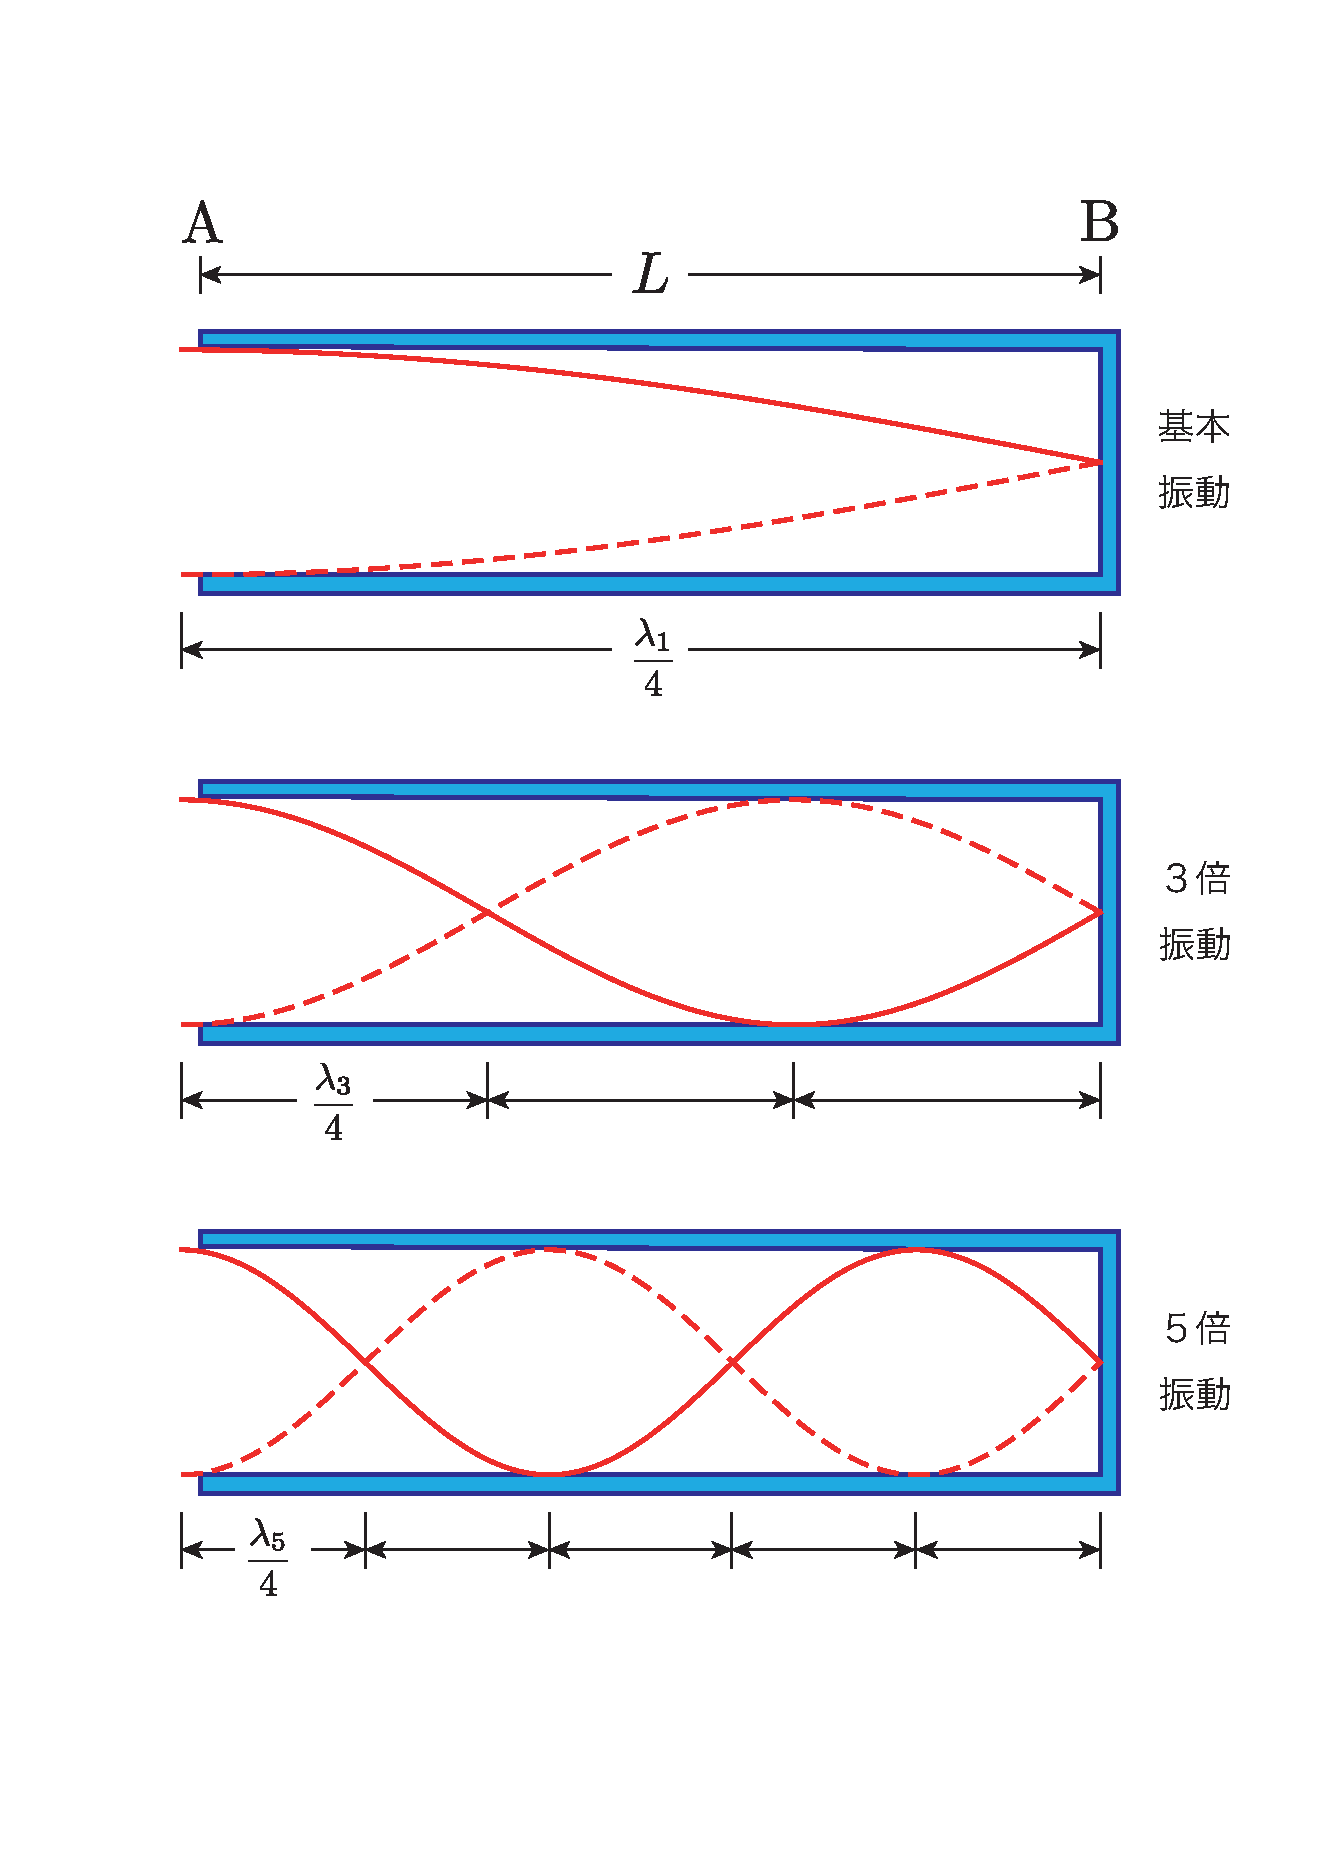
\includegraphics[scale=0.4]{18_Resonance/AirColumn.eps}\\
気柱(閉管)の固有振動\\
\end{center}
\end{wrapfigure}


スピーカーを使って閉管に入れた音の振動数を変化させると、いくつかの決まった振動数で音が強く響き({\bf 共鳴})、
気柱に定常波が発生します。スピーカーから出た音と閉管の閉じた端から反射した音が重なり合って定常波が発生するためには、
長さ$L$の気柱に、波長の$\frac{1}{4}$の長さがちょうど奇数個分入る必要があります(右図参照)。

音波が気柱に定常波を作るとき、開口端では空気が自由に振動できる自由端であるため、「腹」
となります。(空気が自由に移動できるということは、管の外の空気と同じとなるため、
腹の周りでは空気の密度変化が最も小さくなります。)
一方、閉口端では空気が振動できないため、その周りでは空気の密度変化が最も大きい「節」となります。

気柱が共鳴を起こしているとき、最も小さい振動数$\nu_1$では、開口端と閉口端だけで腹と節が生じます。このときの固有振動を
{\bf 基本振動}といいます。

振動数を大きくしていくと、基本振動数$\nu_1$ の3倍、5倍、7倍、$\cdots$となったときに
管の両端以外にも図のような腹と節が発生します。このときを、それぞれ、
3倍振動、5倍振動、7倍振動、$\cdots$と呼びます。

\subsection{空気中の音の速さ}

$n$倍振動($n=1,3,5,7,\cdots$)が発生したとき、節と節の間隔や腹と腹の間隔を測定すると、その間隔は音波の波長の
ちょうど半分になっているので、音波の波長を求めることができます。また、気柱の長さからでも波長を求めることが
できますが、開口端側の腹の位置は管の外側にややずれているため、注意(開口端補正)が必要です。
(振動数を固定し、異なる$n$倍振動が発生したときの管の長さを複数回測定することで開口端補正をすることができます。)

$n$倍振動時の気柱の固有振動数$\nu_n$と、そのときの波長$\lambda_n$がわかれば、波の振動数、波長、速度の関係から、
音速を
\[
v = \lambda_n \nu_n
\]
で求めることができます。

ちなみに、音速は気温$t$ [${}^\circ$C]、1気圧の乾燥空気のもとで、
\[
v = 331.5 + 0.61 t \quad \text{[m/s]}
\]
と近似的に表されることが知られています。

%実験では、共鳴管を用い固有振動を発生させ、そのときの波長から音速を求めます。

\newpage

\jikken

\begin{itemsquarebox}[c]{\bf 実験用具}
発泡スチロール球入り共鳴管、スピーカー、発振器、バナナプラグ付きリード線
\end{itemsquarebox}

\bigskip

\subjikken{音速の測定(気柱の長さ固定)}

\begin{enumerate}

\item ピストンを移動させ、気柱の長さを適当な値に設定します。

\item 発振器の振動数を変化させ、3倍振動、5倍振動、7倍振動、$\cdots$の固有振動状態
(音がよく響き、発泡スチロール球でできる山が大きい状態)を作り、観察します。

\item それぞれの固有振動状態に対して、節と節の間隔や、腹と腹の間隔から波長(間隔の長さの2倍)を求めます。

\item 固有振動の振動数と波長から音速を求め、気温から求めた音速と比較します。

\end{enumerate}

\subjikken{音速の測定(振動数固定)}

\begin{enumerate}

\item 発振器の振動数を固定(1000Hz程度)し、気柱の長さを最も短くした状態から、固有振動状態を作っていきます。

\item $n$倍振動が発生した状態での気柱の長さを$L_n$として測定します。

\item 波長をそれぞれの固有振動状態での気柱の長さの差から求めます。\\(例:$\lambda=2(L_7-L_5)$)

\item 発振器の振動数と波長から音速を求め、気温から求めた音速と比較します。

\end{enumerate}


%!TEX root = ../main.tex
%
% オシロスコープ
%

\section{オシロスコープ}

\subsection{オシロスコープとは}

オシロスコープは、画面の横軸を時間、縦軸を電圧として、電圧の時間変化を表示する装置です。従って、電圧が一定であるようなDC(直流)の場合は
横に延びた時間変動のない直線が表示され、AC(交流)の場合は電圧が周期的に変化するグラフが表示されます。

オシロスコープを用いれば、非常に短い時間の電圧変化を捉えることができ、他の装置と組み合わせることによって様々な測定に用いたり、
電気回路の特性を調べたりすることができます。

%オシロスコープは、電気信号の波形観測を行うための測定器です。これによって、交流電流など、電気信号の時間的変化を観測することができます。もちろん、直流電流の電圧を測定することも可能です。

ここでは、2つの電気信号を入力し観測することができる2現象オシロスコープの使い方を学び、交流信号の周期や周波数を求めると同時に、波の合成について学習しましょう。




\subsection{基本的な動作}

オシロスコープにはブラウン管を使ったタイプのものや、
信号をデジタル的に処理して液晶ディスプレイに表示するタイプのものなど
様々な種類があります。
古くはブラウン管を使ったものが主流でしたが、電気回路が半導体などのデジタル素子を使っているものが
主流となったため、アナログ信号をデジタル信号に変換(A/D変換)して処理するものが多くなっています。

今回の実験で用いるオシロスコープ(PicoScope)は、
外部装置側で電圧をA/D変換してメモリに蓄積し、
デジタル処理されたデータをUSBインターフェイスを通じてパソコン側のソフトウェアで読み取り、表示するタイプのものです。
このタイプのオシロスコープは、処理の一部と表示(液晶ディスプレイ)をパソコンで行うため価格を比較的抑えることができる
利点がありますが、
パソコンやUSB通信の処理速度を超えた信号変化には追随できないという欠点があります。


\begin{enumerate}

\item オシロスコープの使い方

\begin{itemize}

\item パソコンとUSBケーブルを使って接続する。

\item デスクトップのアイコンをダブルクリックして、オシロスコープ用ソフトウェア「PicoScope 7 T\&M」を起動する。

%\item みの虫クリップ付きBNCケーブルを接続する。(チャンネルAまたはB)

\item みの虫クリップ付きケーブルなどを使って、チャンネルAまたはBのBNCコネクタに発振器もしくはマイクを接続する。

\item 「トリガー」をクリックし、モードを「なし」に設定する。

%\item サンプル数を「100 kS」、入力レンジを「自動」、カップリングを「DC」に設定する。

\item 入力チャンネルAまたはBをクリックし、入力レンジを「自動」、カップリングを「DC」に設定する。(使用しないチャンネルは「オフ」にする。)

\item 画面上部の「Scope」に「+/-」ボタンを使って、タイムベース(横軸の1目盛が表す時間)をセットする。
(音叉や音声を測定する場合には1 [ms/div]〜5 [ms/div]の値にセットする。)

%\item うまく波形が出ない場合は、発振器や音を流した状態で「AUTOSET」を押して調整する。

\item うまく波形が出たら、「スペースキー」または「実行/停止ボタン」を押して画面を固定する。

\item 印刷メニューから波形を印刷する。

\item リサジュー図形(XY表示)は、画面上部の「計測」をクリックし、「XY」を選択することで表示できる。
その際、タイムベースを5 [ms/div]に設定する。

\end{itemize}

\item 発振器の使い方

\begin{itemize}

\item コンセントにつなぎ、右下の電源スイッチを入れる。

\item 「減衰器(ATTENUATOR)」を-20 [dB]、「振幅(AMPLITUDE)」ダイヤルを真ん中あたりに設定する。

\item ダイアルと右のボタンの倍率を組み合わせて、出力周波数を100 [Hz]に設定する。


\end{itemize}


\end{enumerate}


\newpage

\subsection{リサジュー図形を見る}

基本の動作では、各チャンネルに入れた信号を、横軸に時間、縦軸に電圧をとって 
表示させましたが、2現象オシロスコープでは、2つのチャンネルに入力された信号を、 片方は縦軸に電圧をとり、もう一方は横軸に電圧をとって、合成して表示することも可能です。この時に現れる図形をリサジュー図形といいます。
%この場合は、軸の調整は、縦軸、横軸共に電圧(Volts/div)のダイヤルで行います。


リサジュー図形を見ることによって、二つの電気信号の周波数の比率、位相の差を 
測定することができます。$\Rightarrow${\bf [実験 5-2]}

\begin{center}
\begin{tabular}{c|ccccc}
& \multicolumn{5}{c}{位相差} \\
周波数比 & $0^\circ$ & $45^\circ$ & $90^\circ$ & $135^\circ$ & $180^\circ$ \\
\hline
\begin{minipage}[b]{5mm}
1:1\\
\end{minipage} &
\includegraphics[scale=0.2]{05_Oscilloscope/1-1.eps} &
\includegraphics[scale=0.2]{05_Oscilloscope/1-2.eps} &
\includegraphics[scale=0.2]{05_Oscilloscope/1-3.eps} &
\includegraphics[scale=0.2]{05_Oscilloscope/1-4.eps} &
\includegraphics[scale=0.2]{05_Oscilloscope/1-5.eps} \\
&&&&&\\
\begin{minipage}[b]{5mm}
1:2\\
\end{minipage} &
\includegraphics[scale=0.2]{05_Oscilloscope/2-1.eps} &
\includegraphics[scale=0.2]{05_Oscilloscope/2-2.eps} &
\includegraphics[scale=0.2]{05_Oscilloscope/2-3.eps} &
\includegraphics[scale=0.2]{05_Oscilloscope/2-4.eps} &
\includegraphics[scale=0.2]{05_Oscilloscope/2-5.eps} \\
&&&&&\\
\begin{minipage}[b]{5mm}
1:3\\
\end{minipage} &
\includegraphics[scale=0.2]{05_Oscilloscope/3-1.eps} &
\includegraphics[scale=0.2]{05_Oscilloscope/3-2.eps} &
\includegraphics[scale=0.2]{05_Oscilloscope/3-3.eps} &
\includegraphics[scale=0.2]{05_Oscilloscope/3-4.eps} &
\includegraphics[scale=0.2]{05_Oscilloscope/3-5.eps} \\
&&&&&\\
\begin{minipage}[b]{5mm}
2:3\\
\end{minipage} &
\includegraphics[scale=0.2]{05_Oscilloscope/4-1.eps} &
\includegraphics[scale=0.2]{05_Oscilloscope/4-2.eps} &
\includegraphics[scale=0.2]{05_Oscilloscope/4-3.eps} &
\includegraphics[scale=0.2]{05_Oscilloscope/4-4.eps} &
\includegraphics[scale=0.2]{05_Oscilloscope/4-5.eps} \\
\end{tabular}
\end{center}

\newpage

\jikken

\begin{itemsquarebox}[c]{\bf 実験用具}
USB接続オシロスコープ(PicoScope)、発振器2台、音叉、マイク
\end{itemsquarebox}

\bigskip

\subjikken{1つの波形の観察}

\begin{enumerate}

\item 発振器からの100 [Hz]の正弦波を、オシロスコープのチャンネルAに入
力し、波形を観察しましょう。また、パソコンに表示された波形のデータを印刷します。波形から、波の周期:$T$ [s]を読
み取り、$\nu=1/T$より、波の周波数を求めることができます。入力信号の周波
数を計算し、100 [Hz]になっていることを確かめましょう。

\item マイクをオシロスコープのチャンネルAにつなぎます。
マイクの前で音叉をたたき、音波の波形がオシロスコープの画面に表示さ
れることを確かめます。次に、マイクに向かって声を出し、声の波形を
表示させ観察しましょう。
波形のデータを印刷したものから、この声の周期$T$ [s]を読み取
り、自分達の声の周波数を求めてみましょう。

\item 周波数がわずかに異なる2個の音叉を同時にたたいてうなりを発生させ、
オシロスコープでその波形を観察してみましょう。
(うなりが見えるように「収集時間」を調整する必要があります。)
また、オシロスコープの表示画面からうなりの振動数を
求めてみましょう。(音叉の振動部分におもりを取り付けることで振動数をずらすことができます。)
2個の音叉それぞれの振動数とうなりの振動数の間にはどのような関係があるでしょうか。

※ マイクは音叉の共鳴箱の開口部に近づけると大きな音を拾うことができます。

\end{enumerate}


\subjikken{リサジュー図形の観察と音叉の周波数の測定}

\begin{enumerate}

\item 2台の発振器から同じ周波数の信号(100 [Hz]でよい)をチャンネルA、チャンネルBに入力し、XY表示に切り替えて、チャンネルAとチャンネルBの波の大きさが大体同じになるように「入力レンジ」を調整します。
また、図形が流れたり動く時は発信器の周波数を微調整します。

\item 表示されたリサジュー図形を観察しましょう。また、
そのまま通常の表示(横軸が時間)に切り替えて、同様に記録し、2つの波形の
位相のずれを観察し、リサジュー図形の形と照らし合わせてみましょう。

\item 同様に、発振器からの信号が1:2のときと、1:3のとき(100 [Hz]と200[Hz]、 
100 [Hz]と300 [Hz]でよい)についてもリサジュー図形を表示させ、
リサジュー図形と2つの波形を比較しましょう。
(プリンターで印刷して比較しても良い。)

\item 次に、リサジュー図形を利用して、音叉の周波数を測定してみましょう。チャンネルAに
はマイクをつなぎ、チャンネルBは発振器をつないだままにし
て、マイクの前で音叉をたたきます。発振器の周波数を変えて、1:1の周波数
の場合のリサジュー図形が表示されるところを探し、音叉の周波数を求めましょ
う。


\end{enumerate}


%!TEX root = ../main_wo_rep.tex
%
% 光の性質
%


\section{光の性質}

\subsection{光の波動性}

\begin{itemize}

\item 光は光速度$c$の速さで伝わる波です。\\
(真空中の光速度:$c=2.99792458\times 10^8$ [m/s])\\
性質1. 横波です。\\
性質2. 他の波と同様に、屈折、反射、回折、干渉が起きます。\\
性質3. 他の波と異なり、真空中(媒質が無い所)でも伝わります。

\item 人間の目は、光のうち波長が約400 [nm]〜約800 [nm]のものを「色」で区別するこ
とができ、波長の長い光は赤色、波長の短い光は紫として認識します。\\
$\Rightarrow${\bf [実験 2-1, 2-2]}

\begin{center}
\includegraphics[scale=0.6, bb=0 0 660 218]{02_Refraction/spectrum.pdf}
\end{center}

\end{itemize}



\bigskip

\begin{itembox}[l]{\bf コラム:光速度より遅い光}
光速度$c=2.99792458\times 10^8$ [m/s]は真空中を進む光の速度です。物質中を進む光の速 
度は光速度$c$より遅くなります。光は速過ぎて(1秒間に地球を7周半もする速さ!)扱いづら 
いので、光をできるだけゆっくり進むようにさせたいという研究が行われています。今の 
ところ、実験段階で達成された一番遅い光の速度は、シリコンを主とした物質内を通る 
光の速度で、真空中の光速度$c$の300分の1ほどしかありません。
\end{itembox}

\newpage

\subsection{光の反射と屈折}

\subsubsection{屈折率}

\begin{wrapfigure}[8]{r}{5cm}
\vspace*{-0.8cm}
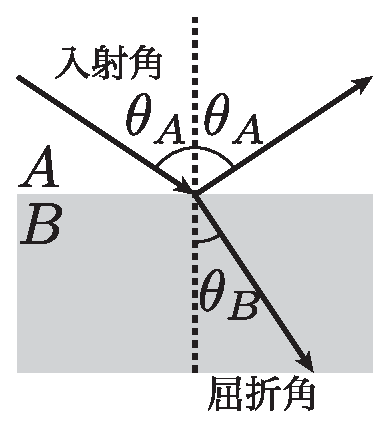
\includegraphics[scale=0.8]{02_Refraction/refraction.eps}
\end{wrapfigure}


密度の違う2つの媒質A、Bが隣り合っているとします。光が媒質Aから媒質Bの方
向に、斜めに入射する場合を考えましょう。

光の一部はAとBの境界面で反射し、また一部は屈折・透過して媒質Bの中を進みます。この時の、
媒質BのAに対する屈折率は次のようになります。
\[
n_{\rm AB} = \frac{n_{\rm B}}{n_{\rm A}} = \frac{\sin \theta_A}{\sin \theta_B}
\qquad
\left(
n_{\rm BA} = \frac{n_{\rm A}}{n_{\rm B}}=\frac{1}{n_{\rm AB}}
\right)
\]
\begin{eqnarray}
n_{\rm A} & \cdots & \text{媒質Aの絶対屈折率(真空に対する屈折率)}\nonumber\\
n_{\rm B} & \cdots & \text{媒質Bの絶対屈折率}\nonumber
\end{eqnarray}
ただし、空気の絶対屈折率は、$n = 1.0003$なので、$n=1$として計算してかまいません。
([媒質の空気に対する屈折率]=[媒質の絶対屈折率] と考えて良い。)

屈折率は光の波長によって異なり、波長が短い光ほど屈折率が大きくなります。すなわち、
赤い光よりも紫の光の方が大きく屈折します。$\Rightarrow${\bf [実験 2-1, 2-2]}

\subsubsection{全反射}

光を、屈折率の大きい媒質Aから屈折率の小さい媒質Bに向けて入射させることを
考えてみましょう。この場合は、入射角より屈折角の方が大きくなります。このとき、入射角が小
さいうちは、入射光の多くは屈折していきますが、入射角を大きくしていくと、ある角度
で屈折角が$90^\circ$になり、これより大きい入射角では光線は媒質Aに進入できず、全
て境界面で反射するようになります。これを{\bf 全反射}といいます。$\Rightarrow${\bf [実験 2-3, 2-4]}

全反射(屈折角が$90^\circ$より大きくなる)が起こるようになる入射角を{\bf 臨界角}といいます。臨界
角は次の式で求められます。$\Rightarrow${\bf[実験 2-4]} 
\begin{eqnarray}
&&n_{\rm A}\sin\theta_A = n_{\rm B} \sin 90^\circ\nonumber\\
&& \Rightarrow \sin\theta_A = \frac{n_{\rm B}}{n_{\rm A}}\nonumber
\end{eqnarray}

\subsubsection{糖度計}

糖度計は測定対象となる液体に含まれる糖の含有量によって光の屈折率が異なる事を利用して
果物等の糖度を測定する装置です。正確には屈折糖度計と呼びます。
糖度とは液体に含まれるショ糖の質量パーセント濃度のことで、Brix\%(ブリックス)
という単位で表します。レモンのように糖度が高くても酸味が強ければ、それほど
甘く感じないので、糖度が感覚的な甘さを表すとは限りません。


\begin{figure}[h]
\begin{center}
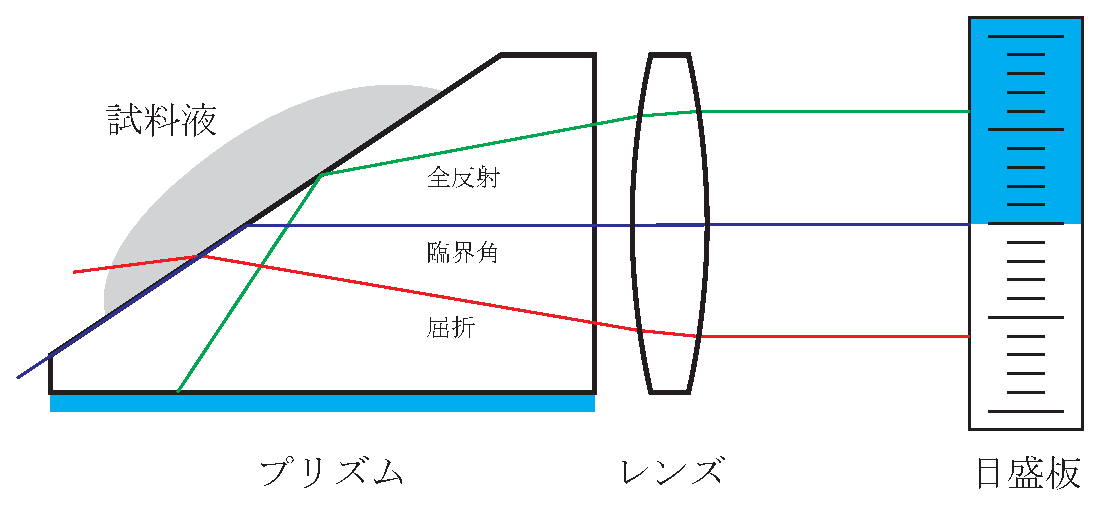
\includegraphics[scale=0.75]{02_Refraction/brix.eps}
\end{center}
\caption{糖度計の仕組み}
\end{figure}

\subsubsection{偏光}

光は進行方向に対して垂直に振動する横波であり、その振動方向が偏ったものを{\bf 偏光}と呼びます。
太陽光などの自然の光は振動方向がまちまちで偏光していませんが、偏光子
と呼ばれる特別な材質のものに光を透過させると、特定の偏光の成分を取り出すことができます。

偏光子を通した光は振動方向が特定の方向になっており、その光をもう一度偏光子を通した場合、
相対的な偏光の方向によって明るさが変化します。
このような偏光の性質を用いて、光の透過率を電気的にコントロールすることができ、
偏光は液晶ディスプレイなどに応用されています。

偏光子には方解石など自然に産出される物質もありますが、現在では偏光フィルムのように
高分子を用いて、安く大量に作ることができるようになり、工業的な利用が進んでいます。




\bigskip
\bigskip

\begin{itembox}[l]{\bf コラム1:光海底ケーブル}
光海底ケーブルは、複数本の光ファイバーケーブルをアルミニウムや鉄芯で耐圧性を高
めたものにポリエチレンで覆いをしたものです。世界中で約80万[km]ものケーブ
ルが海底に巡らせてあります。2005年の時点で、太平洋を横断している光海底ケーブルのシ
ステムは6つで、その全容量は10[Tbps]にも達しますが、そのうち実際に使用されてい
るのは1[Tbps]にとどまっているのが現状です。島国である日本の国際通信の多くは
このような海底ケーブルを利用して行われています。\\
 ※1[Tbps] =1,000,000,000,000 [bps] = 1,000,000,000,000 [ビット/秒] 
\end{itembox}

\bigskip

\begin{itembox}[l]{\bf コラム2:いろいろな糖度計}
屈折糖度計の他にも糖度を測る方法がいろいろあります。旋光糖度計は、ショ糖に
特定の偏光を持った光を通すとその光の偏光面を$66.5^\circ$回転させるという
旋光性を利用して糖度を測るものです。近赤外光糖度計は、ショ糖が近赤外光を吸収する
性質を利用して近赤外光の吸収度合いを測定して糖度を求めるものです。
果物などの作物の糖度を測る場合、屈折糖度計も旋光糖度計もサンプルを傷つけ果汁
を絞り取る必要がありますが、近赤外糖度計はサンプルを傷つけることなく糖度を測定できるので、
分光技術の進歩にともなう装置の小型化と相まって、利用が広がっています。
\end{itembox}

\newpage

\jikken

\begin{itemsquarebox}[c]{\bf 実験用具}
分光用プリズム、白熱灯光源装置、半導体レーザー光源装置、アクリルブロック、
光ファイバー結束線、ファイバースコープ、
光学水槽、糖度計、偏光フィルム、セロハンテープ、方解石
\end{itemsquarebox}

\bigskip

\subjikken{白色光}

太陽光や白熱灯の光は多くの異なる波長の光を含んでいます。白熱灯光源装置の光
をプリズムに入射させると、波長の異なる波は、屈折率の違いによって分散します。
この分散した波長スペクトルを白壁に投影して観察してみましょう。
正三角形のプリズムと直角のプリズムでスペクトルの現れ方(色の順番)に違いが出るでしょうか?
\begin{center}
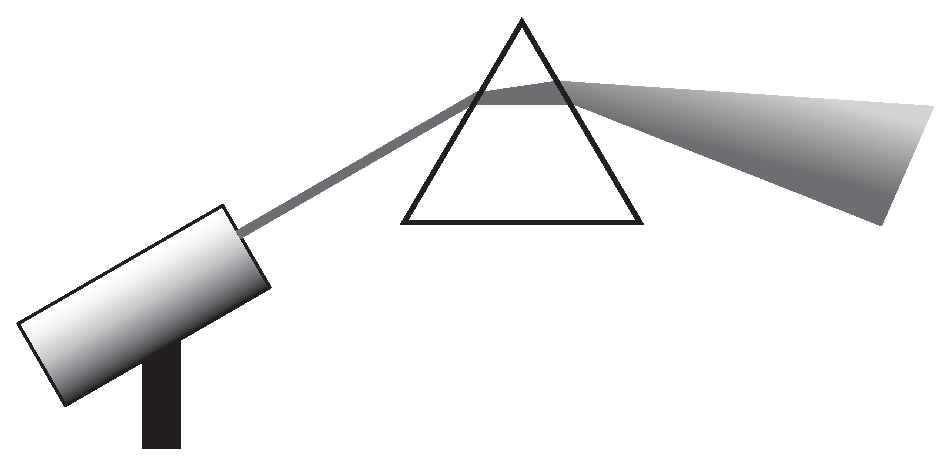
\includegraphics[scale=0.4]{02_Refraction/prism.eps}
\end{center}


\subjikken{単色光}

レーザー光は、ある特定の波長の光のみを、ビームとして出しています。レーザー
光源装置の光を、{\bf [実験 \thesection-1]}と同様に、プリズムを通して観察し、レーザー光が
単一波長の光(単色光)であることを確かめましょう。

\bigskip


\subjikken{光の屈折と反射}

様々な形をしたアクリルブロックにレーザー光を入射させて反射と屈折の法則を確認しましょう。

\bigskip

\subjikken{光ファイバー}

細長い、あるいはS字型のアクリル棒を使って、レーザー光が内部で全反射を起こすこと(条件)を確かめましょう。この光ファイバーの原理を応用した光ファイバー結束線やファイバースコープを使って、光ファイバーの働きを確認しましょう。

\bigskip

\subjikken{臨界角}

光学水槽を用いて、水中から空気中に向けてレーザー光を入射させ、全反射が起こ
ることを確かめましょう。また、このときの臨界角を読み取り、水の屈折率を求めま
しょう。

\bigskip


\newpage

\subjikken{糖度計}

糖度計を用いてコーラやジュースの糖度を計ってみましょう。液体のサンプルをスポイトを使って
糖度計のプリズム面に少量たらし、ふたをしてサンプルがプリズム面に均一に行き渡るようにします。
糖度計を水平に保ちながら接眼部からのぞき、青と白の境界線の目盛の数値から糖度(Brix)
を読み取りましょう。

\bigskip


\subjikken{偏光フィルム}

偏光フィルムを2枚用意して重ね合わせ光が透過する様子を観察しましょう。
重ね合う角度を変化させると透過する光の明るさはどうなるでしょうか。
携帯電話の液晶画面、方解石、様々なものを反射した光などを偏光フィルムを通して見てみましょう。
また、2枚の偏光フィルムの間にセロファン(セロファンテープ)を
重ねて挟んで色や明るさの変化を見てみましょう。

\bigskip



\hspace*{-\parindent}
{\bf 注意}:\underline{レーザー光源を直接目に入れてはいけません。}(ビームの出口をのぞき込まな 
いこと!) 間違って他人の顔の方向にレーザー光を向けてしまわないように、
ビームの出る方向に人がいないことを確認してから電源を入れるようにしましょう。



%!TEX root = ../main.tex
%
% 光の干渉
%


\section{光の干渉}

\subsection{波としての光の性質}

前の章で述べたように光の正体は電磁波という「波」です。光の持つ反射や屈折等の性質を調べても光が波の性質を
持つ事は実感できませんが、光の経路をスリット等を使って分けた後に再び重ね合わせると水の波の実験で見た様な
「干渉」という波が持つ特有の現象を観察することができます。

この章の実験では干渉をおこしやすい性質を持つレーザー光を用い、ダブルスリットや回折格子で光がどのように
して干渉をおこすのか調べ、その結果からレーザー光の波長を求めます。

\subsection{単スリット}

\begin{wrapfigure}[6]{r}{7cm}
\vspace*{-0.8cm}
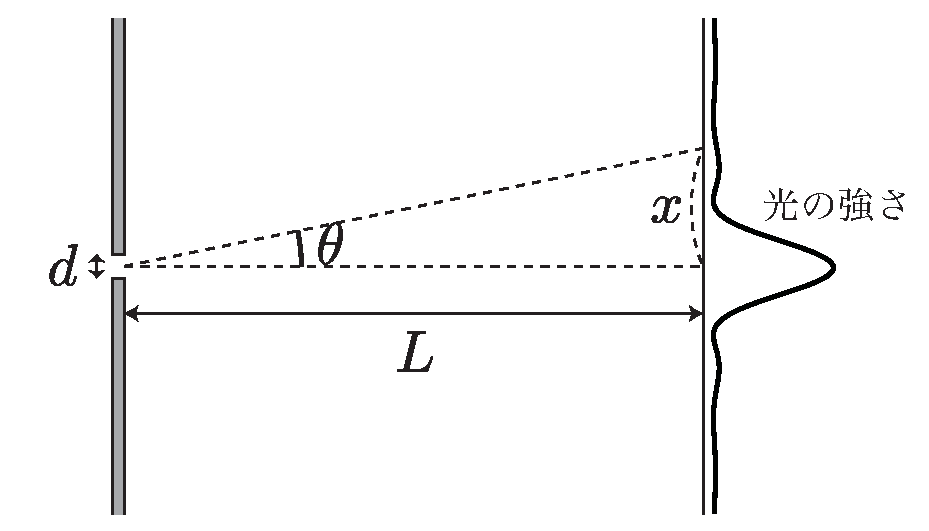
\includegraphics[scale=0.5]{03_Interference/one-slit.eps}
\end{wrapfigure}


まず、幅$d$の単スリットがある障壁を考えてみましょう。この障壁に垂直に入射し、ス
リットを通った波長$\lambda$の光の強度は次の式のようになります。
\[
I(\theta)=I_0
\left|
\frac{\sin\left(\frac{\pi}{\lambda}d\sin\theta\right)}{\frac{\pi}{\lambda}d\sin\theta}
\right|^2
\]

この式から、最初に光が弱くなる($I(\theta)=0$となる)のは、
\begin{equation}
d\sin\theta=\lambda
\label{dark line}
\end{equation}
の時になります。続いて、 
\[
d\sin\theta=2\lambda,~3\lambda,\cdots
\]
のように、波長の整数倍の条件を満たす方向で光が弱まり、暗線が見えます。

また、$\theta=0$の時に光の強度は最大となりますが、他の明線(明るさのピーク)の
条件は一般に求めるのは難しく、
\[
d\sin\theta \simeq \frac{5}{2}\lambda,~\frac{7}{2}\lambda,\cdots
\]
の条件を満たす方向付近に明線が現れます。

%\bigskip
%
%\hspace*{-\parindent}
%※ $\theta=0$の時は、光の強度が最大になることに注意


ここで、図のように、障壁から距離$L$の所
にスクリーンを置きます。スクリーン上で、ス
リットの中心から直進して到達する点から、最初
に光が弱くなる所までの距離を$x$とすると、光の
強度が最初に弱まる所を表わす(\ref{dark line})の式は、$x$に 
比べて$L$が充分に大きい場合には、($\sin\theta\simeq x/L$として)
\begin{equation}
\frac{d\,x}{L}=\lambda
\label{approx dark line}
\end{equation}
と近似して書くことができます。(\ref{approx dark line})
の式から、$d$, $x$, $L$を測定すれば、光の波長$\lambda$が求められます。
%$\Rightarrow${\bf [実験 3-1]}


\subsection{ダブルスリット}


\begin{wrapfigure}[7]{r}{7cm}
%\vspace*{-0.8cm}
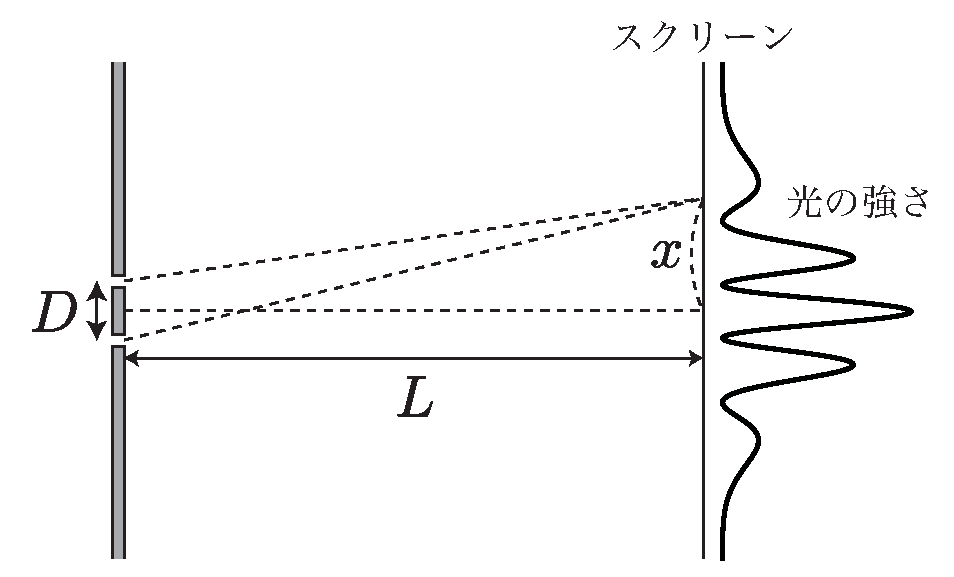
\includegraphics[scale=0.5]{03_Interference/two-slits.eps}
\end{wrapfigure}


まず、細いスリットが二本開いているダブルスリットを考えましょう。
2本のスリットの間隔を$D$とし、スリットの幅は無視できるとします。障壁とスク
リーンの距離を$L$とすると、スクリーン上で中心からの水平
距離が$x$である点における「左スリットから入った光と右ス
リットから入った光が通ってきた道のりの差」=光路差は、
\begin{eqnarray}
光路差&=&\sqrt{L^2+\left(x+\frac{D}{2}\right)^2}
-\sqrt{L^2+\left(x-\frac{D}{2}\right)^2}\nonumber\\
&\simeq& \frac{x\,D}{L}\nonumber
\end{eqnarray}
となります。($x$に比べて$L$が充分に大きい場合。)

光が最も強くなるのは、$x=0$の所になります。それ以降は、
\[
\frac{x\,D}{L}=\lambda,~2\lambda,~3\lambda,\cdots
\]
となる所(光路差がちょうど光の波長の整数倍になる所)で同位相の波の重ね合わせ効果で
光が強められ明線が現れます。$\Rightarrow${\bf [実験 \thesection-1]}

一方、逆位相で光が弱められて暗線が見えるのは、
\[
\frac{x\,D}{L}=\frac{1}{2}\lambda,~\frac{3}{2}\lambda,~\frac{5}{2}\lambda,\cdots
\]
のとき、すなわち、位相が半波長分ずれるときになります。 

\begin{center}
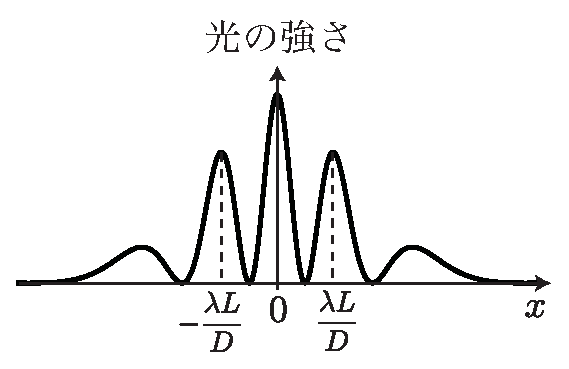
\includegraphics[scale=0.7]{03_Interference/two-slits-int.eps}
\end{center}


\subsection{回折格子}

\begin{wrapfigure}[10]{r}{7cm}
\vspace*{-0.5cm}
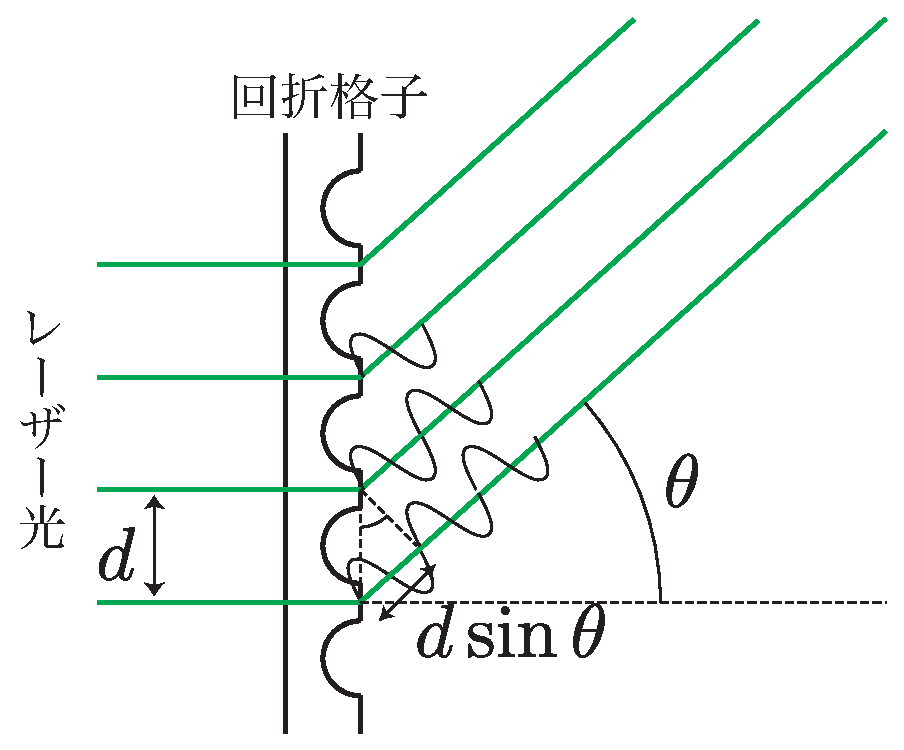
\includegraphics[scale=0.5]{03_Interference/grating.eps}
\end{wrapfigure}


回折格子とはガラス板やプラスチックフィルムに1mmあたり数百本もの細かい溝などの構造を等間隔で刻んだものです。
グレーチングやレプリカフィルム等とも呼ばれます。
細かい構造によって、光が透過する部分と遮られる部分が交互に繰り返し、透過した多数の光どうしが干渉した結果、
波長ごとに光が強められる方向が決まります。数が非常に多いスリットと考えても良いでしょう。

格子の間隔が$d$である回折格子に垂直に光を当てたとき、角度$\theta$で出て行く光どうしの光路差はすべて
\[
d\sin\theta
\]
となるので、この長さが波長の整数倍($\lambda,2\lambda,3\lambda,\cdots$)になるときに光は強め合います。
また、この長さが波長の半整数倍($\frac{1}{2}\lambda,\frac{3}{2}\lambda,\frac{5}{2}\lambda,\cdots$)
のときは光が弱め合う条件となりますが、
回折格子の場合は多数の光どうしで干渉するので、強め合う条件以外の方向に光は出て行くことはほとんどありません。
この結果、レーザーなどの点状の光源を用いた場合、干渉縞は明るい点の列となって現れます。$\Rightarrow${\bf [実験 \thesection-2]}

回折格子からスクリーンまでの距離を$L$、スクリーン上で中心からの水平距離を$x$とすると、
\[
\sin \theta = \frac{x}{\sqrt{x^2+L^2}}
\]
と表され、$x$に比べて$L$が非常に大きい場合は、
\[
\sin \theta = \frac{x}{\sqrt{x^2+L^2}} \simeq \frac{x}{L}
\]
と近似できますので、これらを用いて明線(明点)の位置を決定したり、逆に明線の位置から
光の波長を求めることができます。






\newpage

\jikken

\begin{itemsquarebox}[c]{\bf 実験用具}
He-Neレーザー光源(赤色)、半導体レーザー光源(赤色、緑色)、光学台、ダブルスリット板、
回折格子、CD、定規又は巻尺
\end{itemsquarebox}

\bigskip

%\subjikken{単スリットを用いた干渉縞の観察}

%\begin{enumerate}
%
%\item レーザー光源装置を架台の上に設置し、設置したスクリーン(方眼紙を使用)の
%中央に、レーザー光が当たるように高さを調節します。
%
%\item レーザー光源と方眼紙の距離を1 [m]以上離して設置しておきます。
%
%\item レーザー光源のビームの出口にある切り込みに、単スリット板を設置し、このス
%リットを通ったレーザー光により、スクリーン上に生じる干渉模様を観察しましょ
%う。干渉縞の最初の暗点と中心の明点の距離$x$、スリット板からスクリーンまで
%の距離$L$を測定し、スリットの幅$d$を考慮して、レーザー光の波長をそれぞれの
%スリット板について計算しましょう。
%
%
%\end{enumerate}

\subjikken{ダブルスリットを用いた干渉縞の観察}

\begin{enumerate}

\item レーザー光源装置を架台の上に設置し、設置したスクリーン(方眼紙を使用)の
中央に、レーザー光が当たるように高さを調節します。

\item レーザー光源と方眼紙の距離を1 [m]以上離して設置しておきます。

\item レーザー光源の前にスリットの間隔が0.1 [mm]および
0.2 [mm]の ダブルスリット板を設置し、このス
リットを通ったレーザー光により、スクリーン上に生じる干渉模様を観察しましょ
う。

\item 干渉縞の中心の明点と2番目の明点との距離$x$ [mm]、スリット板からスクリーンまで
の距離$L$ [mm]を測定し、スリットの幅$d$ [mm]を考慮して、
赤色と緑色のレーザー光の波長をそれぞれの
スリット板について計算しましょう。


\end{enumerate}



\bigskip

\subjikken{回折格子による干渉実験}

縦方向に一定間隔で細かい筋がたくさんついた回折格子を通すと、スクリー
ン上に写し出される干渉模様はどのようになるでしょうか。ダブルスリットでの干渉縞
と比較してみましょう。回折格子についてもダブルスリットのときと同様の実験を行い、
レーザー光の波長を求めてみましょう。

\bigskip


%\subjikken{ピンホールによる干渉実験}
%
%ピンホールや方眼回折格子の場合にはどのような干渉縞ができるでしょうか。
%今までの結果から予想して観察してみましょう。

\subjikken{CDのトラックピッチの測定}

CDには非常に細かい出っ張り(ピット)が刻まれていて、そこに音楽などのデジタルデータが記録されています。
ピットによって反射された光は回折格子と同様の原理で干渉をおこします。
CDにレーザー光線を反射させ、
その干渉縞(明点)の間隔およびCDとスクリーンまでの距離を測定し、
レーザー光線の波長からCDのピット列の間隔(トラックピッチ)を求めてみましょう。


\bigskip


\hspace*{-\parindent}
※ {\bf 注意}:レーザー光源を直接目に入れてはいけません。(ビームの出口をのぞき込まな
いこと。他人の顔の方向にビームを向けないこと。) また、鏡面反射を起こ
すもの(鏡、腕時計など)をビーム付近に近づけないようにしましょう。
%%!TEX root = ../main.tex
%
% ニュートンリング
%


\section{ニュートンリング}

\subsection{ニュートンリング実験器}

ニュートンリングとは、平凸レンズと平面のガラス板を組み合わせ、そこに光を当て
たときに入射光と反射光の干渉効果によって生じるリング状の光の縞模様のことです。
このリングのサイズを測定するための装置がニュートンリング実験器です。
この実験器は、次のような目的に使うことができます。

\begin{enumerate}

\item 波長の分かっている単色光源を用いてニュートンリングを作り、リングの大き
さを測定することによって、レンズの曲率半径を求める。

\item 曲率半径の分かっているレンズを用い、単色光源を当ててニュートンリングを
作り、リングの大きさを測定することによって、単色光源の波長を求める。

\end{enumerate}

\subsection{測定原理}

\begin{wrapfigure}[11]{r}{7cm}
\vspace*{-0.8cm}
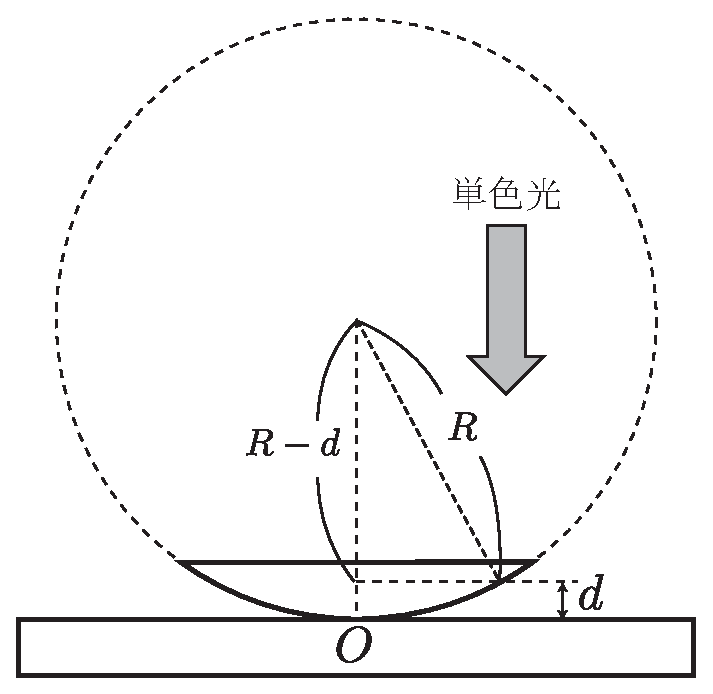
\includegraphics[scale=0.6]{04_Newton/newton.eps}
\end{wrapfigure}


右図のように、平面ガラス板の上に平凸レンズを置くと、凸レンズ面とガラス
板の間に薄い空気の層ができます。

このガラス板に垂直になるように、上面から光が入射したとき、平凸レンズの
下面で反射した光と、平面ガラス板の上面で反射した光が干渉し、干渉縞が生じ
ます 。

右図の点Aの位置に光が入射したときの、平凸レンズと平面ガラスの間の空気の層の厚さを$d$とします。
空気の層は非常に薄いので、入射光と反射光はほぼ平行とみなすことができるため、
入射光と反射光が通った道のりの差(光路差)は、$2d$と表わすことができます。

このことから、レンズの凸面の曲率半径を$R$とし、凸面とガラス面との接点Oから 
光の入射点までの距離を$r$とすると、次の関係式が成り立ちます。
\begin{eqnarray}
&&r^2 = R^2-(R-d)^2 = 2Rd-d^2\approx 2Rd\nonumber\\
&&\Rightarrow 2d=\frac{r^2}{R}\nonumber
\end{eqnarray}


平面ガラスの上面での光の反射は、空気からガラスへ向かう境界面での反射なので、
(ガラスの方が光学的に密であるため)固定端の反射となり、位相が反転します。その
ため、光路差が光の波長$\lambda$の整数倍のときは、入射光と反射光は逆位相で干渉して暗くな
ります。この時の$r$と$R$, $\lambda$との関係は次のようになります。
\begin{eqnarray}
&&\frac{r^2}{R}=m\lambda\nonumber\\
&&\Rightarrow r^2=m\lambda R
\qquad (m=0,1,2,3,\ldots)\nonumber
\end{eqnarray}
この条件を満たす位置を上方から見ると、点Oを中心とした暗い円が観測されることになります。

実際にはレンズの凸面とガラスの平面が正確に中心で接していないことから、そのず
れの大きさを$\delta$とおくと、光路差は$2(d+\delta)$となり、先ほどの暗い円が見られるための
条件式は、
\[
r^2 = m\lambda R-2\delta R
\]
となるので、中心から$m$番目の円の半径$r_m$と$m+n$番目の半径$r_{m+n}$を求めると、
このずれの大きさを消去してやることができます。
\[
\left\{
\begin{array}{l}
r_m^2=m\lambda R-2\delta R\\
r_{m+n}^2=(m+n)\lambda R-2\delta R
\end{array}
\right.
\] 
\begin{equation}
\Rightarrow
\boxed{
\lambda R =\frac{r_{m+n}^2 - r_m^2}{n}
}
\label{Newton}
\end{equation}
実際の測定ではこの式を用いて計算を行います。$\Rightarrow${\bf [実験 4-1]}


\newpage

\jikken

\begin{itemsquarebox}[c]{\bf 実験用具}
ニュートンリング実験器(マイクロメーターつき顕微鏡、ニュートンリング板 、
ハーフミラー)、ナトリウムランプ
\end{itemsquarebox}

\bigskip

\subjikken{ニュートンリング実験器による単色光の波長の測定}


ニュートンリング実験器は、マイクロメーターつきの
移動顕微鏡、ハーフミラー、ニュートンリング板(平
凸レンズと平面ガラスを合わせたもの)をセットした
レンズ容器の支持台で構成されています。顕微鏡の倍
率は約10倍で、マイクロメーターで左右に移動する
ことができます。

\begin{enumerate}

\item 平凸レンズの凸面を下にして平面ガラスの上に重
ね、レンズ容器に入れてレンズ支持台に固定してお
きます。(通常は最初からセットしてあります。)

\item ナトリウムランプを点灯し、その光を$45^\circ$に傾け
たハーフミラーに入射させてガラス板に当てます。
光が当たると、肉眼でもレンズの中心付近に小さな
ニュートンリングが見えます。

\item 最初に顕微鏡の接眼部を回して顕微鏡の視野の十字線のピントを合わせます。
十字線がはっきり見えたら、これ以降接眼部はさわらないようにします。

\item マイクロメーターの目盛りは0〜25 [mm] なので、最初は目盛りの中心辺りの
12 [mm]付近に目盛りを合わせ、このとき十字線の中心にニュートンリングの中心
が来るように、レンズ容器の位置を調節してやります。

\item 測定は、誤差を少なくするため、暗円の直径を測定して半径を算出する方法を用
います。中心の黒丸を0番目とし、次の暗線を1番目として数えていき、5番目
以降の輪の直径を測定し、10番目の輪の直径まで、以下に述べるような順序で測
定を行ないます。また、マイクロメーターは逆回転させる際に誤差が生じやすい
ため、測定中は必ず一方方向にだけ、つまみを回していくようにします。

\begin{enumerate}

\item まず10番目の輪の左側の線に十字線の中心を合わせて、その時のマイク 
ロメーターの値:$a_{10}$を読み取り、記録します。(10番目の輪が見えない 
場合は、測定可能な輪のうち一番外側の輪の左側に合わせます。)

\item マイクロメーターを動かして十字線の中心を少しずつ右にずらし、9番目 
の輪、8番目の輪の左側の線の場所、$a_9$, $a_8$を同様にして測定していき 
ます。

\item 5番目の輪の位置($a_5$)まで記録したら、今度は5番目の輪の右側の線
まで十字線の中心を移動し、この場所:$a_5'$を記録します。同様にして、
10番目の輪の右側の位置:$a_{10}'$まで、順番に測定します。(なるべく外側
の輪のデータを用いた方が正確に測定できるので、見えていれば15番
目の輪の位置まで測定しましょう。)

\item 輪の直径と半径を求めていきます。
\[
2r_5= a_5'-a_5 \quad \Rightarrow \quad r_5=\frac{a_5'-a_5}{2}
\]
のようにして、 $r_5\sim r_{10}$まで、それぞれ半径を求めます。

\item ニュートンリング板の曲率半径を2000 [mm]とし、(\ref{Newton})式を用い
てナトリウムランプの波長λを求めます。$n=3$とし、$m=5, 6, 7$の3通
りについて$\lambda$を計算し、それらの値の平均値を求めましょう。


\end{enumerate}


\end{enumerate}



\hspace*{-\parindent}
※ ナトリウムランプの波長を理科年表で調べ、自分達の測定結果と比較しましょう。


%!TEX root = ../main.tex
%
% 磁場
%


\section{磁場の性質}

\subsection{磁石と磁場}

私達の身の周りでは、多くの磁石が使われています。これらの磁石には、大きく分けて、永久磁石と電磁石という2種類があり、常に磁石の性質を持っているものを永久磁石、電流を流したときだけ磁石になるようなものを電磁石といいます。

棒状の永久磁石の重心のところを糸でつるすと、地磁気の方向を向くことが知られて
います。この棒磁石に鉄粉をふりかけると、両端に多く鉄粉が吸い付くことがわかります。この両端を{\bf 磁極}と呼び、北を指す方の磁極を{\bf N極}、南を指す磁極を{\bf S極}と呼びます。これらの磁極間には力が働きますが、これは、一方の磁極が周囲に{\bf 磁場(磁界)}を作り、もう一方の磁極がその磁場を感じるためである、と考えることができます。このような解釈するのが場という概念を用いた考え方です。

磁場の向きは、磁力線(N極から出てS極へ向かう曲線)によって示され、磁場の強さはその「磁力線の密度」=磁束密度によって表すことができます。磁束密度の単位としては、[gauss](ガウス)や[T](テスラ)などが用いられています。

%\paragraph{問題1:}
%鉄が磁石に引きつけられることはよく知られています。では、鉄以外の物は、
%磁石に対してどのように反応するでしょうか。考えてみましょう。
%
%\paragraph{問題2:}
%永久磁石を使った方が便利な場合と、電磁石を使った方が便利な場合をそれ 
%ぞれ考えてみましょう。

\subsection{磁気ヒステリシス曲線}

\begin{wrapfigure}[16]{r}{7cm}
\vspace*{-0.8cm}
\begin{center}
\includegraphics[scale=0.3]{06_Magnetism/MagneticDomain.eps}\\
強磁性体中の磁区\\
\vspace*{0.5cm}
\includegraphics[scale=0.5]{06_Magnetism/hysteresis.eps}\\
磁気ヒステリシス曲線
\end{center}
\end{wrapfigure}


外部の磁場によって磁気を持ち、磁石になる鉄、ニッケル、コバルトなどの金属を{\bf 強磁性体}と呼びます。
強磁性体の内部は小さな磁石の集合体(磁区)でできていて、外部から磁場を与えると徐々に磁区の磁気の方向が外部の磁場の方向にそろうようになり、
全体として磁気を帯びて磁石になります。外部の磁場を強くしていくと磁石の強さ(磁束密度)もそれに応じて強くなりますが、磁区の方向が
全てそろってしまうと磁束密度の大きさは限界に達します。これを{\bf 飽和磁束密度}といい、その強磁性体を用いた
電磁石の最大の強さとなります。

はじめに磁区の方向がバラバラで全体として磁気を持っていなくても、外部の磁場を一度与えて軸の方向をそろえると、外部の磁場をなくしても
強磁性体には磁気が残ります。この時の磁束密度を{\bf 残留磁束密度}といい、強磁性体を使った永久磁石の強さとなります。
また、外部の磁場を逆に与えて強磁性体の残留磁束密度をゼロにするために必要な外部磁場を{\bf 保磁力}といいます。

外部の磁場と強磁性体が持つ磁束密度の関係を表すグラフのことを磁気ヒステリシス曲線といいます。
磁気ヒステリシス曲線は電磁石や永久磁石、トランスなどの特性を決める上で重要なものとなります。



\bigskip

\begin{itembox}[l]{\bf コラム:古磁気の話}
地球の磁場(地磁気)は、鉄を主成分とする外殻コアー(地下2900〜5100 [km])が液体状になっているため、地球の自転によって発生するものと考えられています。太古の昔に噴出した溶岩が冷えて固まる時に、溶岩に含まれている鉄はその当時の地磁気に従って磁気を得ます。化石等によって地質学的に年代のわかっている岩石の残留磁気を調べることにより、昔の地磁気の様子がわかります($\rightarrow$古地磁気学)。それによると、地磁気は過去に何十回も反転しており、一番最近では70万年前に反転し現在の向きになったと考えられています。また、日本列島は約1500万年前に大陸から分離したことも明らかになりました。
\end{itembox}




\newpage

\jikken

\begin{itemsquarebox}[c]{\bf 実験用具}
各種磁石、立体磁界観察槽、%方位磁針、その他身の回りにあるもの(鉄釘、お札や鉛筆、硬貨など)
磁界観察シート、電磁石コイル、鉄心、テスラメーター、直流安定化電源装置、直流電流計、バナナプラグ付きリード線、セロハンテープ
\end{itemsquarebox}

\bigskip

%\subjikken{}
%
%鉄や、鉄以外の物の磁石に対する反応を、実際に身の回りの物で実験して
%確かめてみましょう。
%
%
%
%\begin{enumerate}
%
%\item 鉄釘は、棒磁石のどこにでも引きつけられるでしょうか。
%
%\item 棒磁石の端に鉄釘をつけ、さらに釘の先に別の釘をつけてみましょう。
%釘は何本までつけられるか、また、なぜ釘の先に別の釘がつけられる
%のかを考えてみましょう。
%
%\end{enumerate}


%\subjikken{}
%
%電磁石のコイルの内側に鉄芯を入れた場合と入れない場合では、電磁石は
%どのように変化するかを確かめましょう。
%
%\bigskip

\subjikken{棒磁石の周りの磁場}

立体磁界観察槽(砂鉄と流動パラフィンの入ったアクリル製観察槽)を使
って、棒磁石によって周りの空間にどのような磁場が生じるのかを観測し、
スケッチしてみましょう。(ただし、磁束線は磁石のN極から外へ出て、
磁石のS極へと戻ってくるとする。) 棒磁石一本のときと、棒磁石二本を
両端から入れた場合についても観察しましょう。

\begin{center}
\begin{tabular}{ccc}
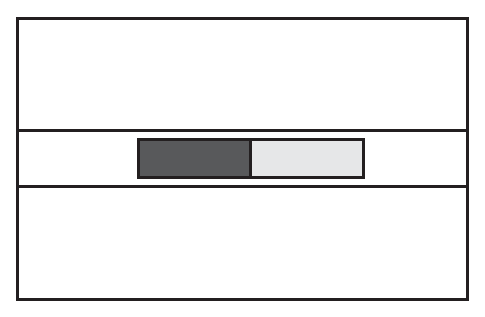
\includegraphics[scale=0.6]{06_Magnetism/magnet1.eps}&\hspace*{5mm}&
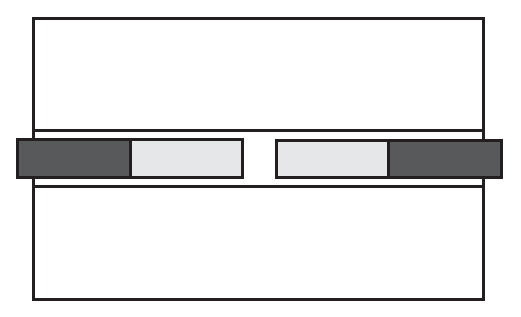
\includegraphics[scale=0.6]{06_Magnetism/magnet2.eps}
\end{tabular}
\end{center}

%\bigskip
%
%\subjikken{}
%
%地磁気の観察をしてみましょう。建物の周りの地磁気を観測し、実際の南
%北との差を調べ、その理由について考察しましょう。

%\bigskip
%\newpage


\subjikken{磁気カード上の磁場の観察}

図書カード、コピーカード、バスカードや電車の切符等にも磁性体が使わ
れています。カードのどこに磁性体がぬってあるか使用済みのカードを
磁界観察シートを使って調べてみましょう。 

\bigskip


\subjikken{磁石の種類による磁力の違い}

テスラメータを使って、アルニコ磁石、ネオジム磁石などの磁力の強さ(磁束密度)を測定して比較してみましょう。
測定する場所や磁石をつなげた時で磁束密度はどのように変化するでしょうか。

%\bigskip
\newpage

\subjikken{ヒステリシス曲線の測定}

\begin{enumerate}

\item 電磁石コイル、安定電源装置、直流電流計($\sim$5[A])を配線します。

\item 電磁石コイルの中に鉄心を入れ、鉄心の先端にテスラメータをセロハンテープで固定します。

\item 「電圧調整(粗・微)」つまみを中央、「電流調整 (粗・微)」を最小にした状態で、直流安定化電源装置の電源を入れます。

\item 電流を0.5[A]単位で5[A]まで増やしつつ、テスラメータの値を読み取り、記録します。同様に、電流を5[A]から0.5[A]
単位で0[A]まで減らしつつ磁束密度を記録します。

\item 電流と磁束密度の関係をグラフにし、磁場と磁化の間にどのような関係があるか考えましょう。
コイルの電流を増やした後、最後に電流をゼロにしても鉄心に磁束密度が残るのはどうしてでしょうか。

\end{enumerate}




%!TEX root = ../main_wo_rep.tex
%
% 電流と磁場
%


\section{電流と磁場}

\subsection{電流が磁場から受ける力と電流が作る磁場}

\begin{wrapfigure}[6]{r}{6cm}
\vspace*{-0.4cm}
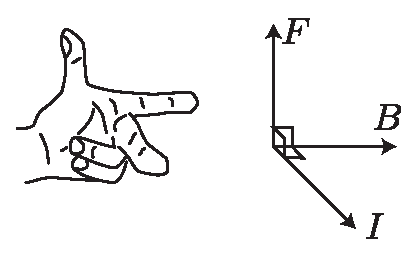
\includegraphics[scale=0.9]{07_EleMag/FBI.eps}
\end{wrapfigure}


動いている電荷(=電流)は磁場から力を受けることが知られています。点電荷$q$が磁
束密度$B$から受ける力は、点電荷が磁場の向きに対して垂直な向きに速度$v$で
動いているとすると、$F=qvB$の大きさの力を受けます。この力を{\bf ローレンツ力}といい、
力を受ける向きは、{\bf フレミングの左手の法則}によって表されます。(電流$I$の向きは、負
の電荷を持つ電子の進む方向とは逆向きなので注意しましょう。)

また、動いている電荷(電流)自身が周囲に磁場を作ることも知られています。電流が
作る磁場の強さを表す法則は、{\bf ビオ・サバールの法則}と呼ばれています。

\subsection{電磁誘導(磁場が作る電流)}

1831年にファラデーは、コイルに磁石を近づけたり遠ざけたりすると、コイルに電
流が流れること発見しました。この現象を{\bf 電磁誘導}といいます。

この現象は、コイルを固定して磁石を動かす代わりに磁場の中でコイルを動かして
も起こり、コイルや回路の中を垂直に貫く磁場の強さが時間的変化をすると、磁場の強
さがどの程度変化するかに応じて流れる電流の量が変わります。

この原理を利用したものには、発電機、変圧器、マイク(ダイナミックマイク)などがあります。


\bigskip

\begin{itembox}[l]{\bf コラム:交流モーターの話}
皆さんが本授業で作るモーターは乾電池で動くもので、直流モーターです。交流電源
に接続しても動きません。このモーターに使われているネオジム磁石を電磁石に置き換
えて電機子と直列に接続すると直流直巻モーターになります。ところが、この種のモーター
は交流でも動くので、一般にユニバーサルモーターと呼ばれていて、扇風機や電気掃除
機等に利用されています。但し、音がうるさいという難点があります。

{\bf 注意:} 皆さんが作成する簡易モーターをユニバーサルモーターに改造してコンセント 
(100ボルトの交流電源)につながないこと。非常に危険です!
\end{itembox}



\newpage

\jikken

\begin{itemsquarebox}[c]{\bf 実験用具}
エナメル線、みの虫クリップの導線2本、単一乾電池、ネオジム磁石、
セロテープ、紙、紙コップ、紙やすり、カッターマット、ミニアンプ、ノートパソコン、
単三乾電池、ブレッドボード、ゼムクリップ(小) 2個、ニッパー
\end{itemsquarebox}

\bigskip

\subjikken{簡易スピーカーの作成}

\begin{enumerate}

\item まず、エナメル線を3 mほど切り取り、単一乾電池に巻きつけてコイルを作ります。コイルの巻
き数は$30\sim 50$回ほどにし、コイルの端はそれぞれ15 cmほどエナメル線を出して
切断しておきます。コイルはケースからはずし、ばらばらにならないように2ケ
所程度をセロテープで軽くとめておきます。

\item 紙コップの底の裏に、コイルをセロテープで貼り付けます。(2ヶ所をとめればよ 
い。)

\item 次に、磁石を別の紙に貼り付け、磁石がコイルの中に入るように注意して、その
紙をコップの裏に貼り付けます。

\item コイルの両端のエナメル線の被膜を、紙やすりではがし、
コイルの両端をミニアンプのスピーカー端子に接続します。

※ 紙やすりで被膜をはがすときは実験机を傷つけないよう、必ずカッターマットの上で作業しましょう。


\item ミニアンプの入力をノートパソコンのイヤホン出力と接続し、
ノートパソコンで音楽を再生します。音量をあげて紙コップを耳に当て、
音が聞こえてくるか、確かめましょう。

\item 磁石の種類を変えたり、ハガキや厚紙などの紙や、紙以外の材質(プラスチック
など)でも試してみて、音が大きくきれいに出せる条件を考えてみましょう。

\item 作成したスピーカーのエナメル線をオシロスコープのCH1に接続し、スピーカーに向かって
声を出してオシロスコープの表示を観察しましょう。
オシロスコープに声の波形が表示されることからスピーカーが
マイクとして作用していることがわかりますが、なぜマイクとして
働くのかについても考えてみましょう。

%\hspace*{-\parindent}
%※ なぜ音が聞こえるのか、考察しましょう。また、まったく同じ仕組みでマイクが
%作れますが、なぜマイクとして働くのかについても考察しましょう。


\end{enumerate}



\newpage

\subjikken{簡易モーターの作成}

\begin{enumerate}

\item エナメル線を50 cmほど切り取り、
エナメル線の端を5 cm程度残して、{\bf 単三乾電池}に10回ほど巻きつけてコイルを
作ります。コイルは巻き始めと巻き終わりの左右の2箇所にエナメル線を巻きつ
けて固定しておきます(2回ほど巻いておけば良い)。下の図のような形になりま
すが、このとき左右のエナメル線がちょうどコイルの中心の高さを通るように気
をつけて作成します。
\begin{center}
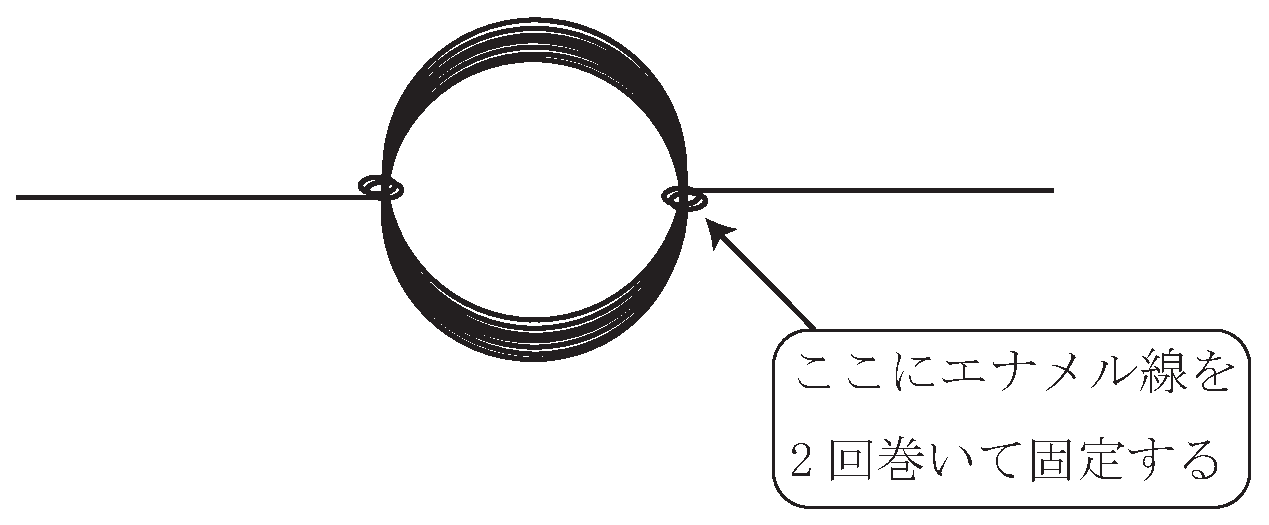
\includegraphics[scale=0.45]{07_EleMag/coil.eps}
\end{center}

\item
\begin{minipage}[t]{10cm}
クリップ2個の先を図のように伸ばし、10$\sim$15個ほどの穴の間隔
をあけて土台にするブレッドボードの穴に刺しておきます。
\end{minipage}
\begin{minipage}[c]{3cm}
\hspace*{1cm}
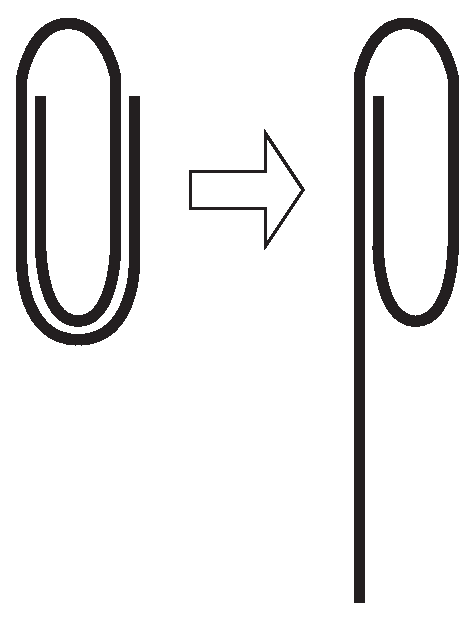
\includegraphics[scale=0.35]{07_EleMag/clip.eps}
\end{minipage}

\item コイルから出ているエナメル線の長さを適当な長さ
(1.5 cm$\sim$2 cm)に切り、先端の1 cmほどを、片方は紙
やすりを使って被膜を全部剥がし、もう一方は半分のみ
剥がしておきます。

※ 紙やすりで被膜をはがすときは実験机を傷つけないよう、必ずカッターマットの上で作業しましょう。


\item ブレッドボードに刺したクリップに通電するように導線をつなぎます。
(ブレッドボードの穴どうしは列単位で電気的に接続されています。)
さらに、クリップとクリップの真ん中に来るように、
ネオジウム磁石をブレッドボードにセロテープでとめておきます。

\item 2本のクリップを軸受けにしてコイルを設置し、ブレッドボードからの導線の
端を乾電池につなぎ、コイルを軽く指で押して回転させてやります。(回転の向き
に注意すること。)

\hspace*{-\parindent}
※ うまくできていれば、そのままコイルは勢い良く回転し続けます。

\item オシロスコープを使ってモーターのコイルにかかる電圧の変化を
観察してみましょう。電圧の変化からどのようなことがわかるでしょうか?

\end{enumerate}


%%!TEX root = ../main.tex
%
% モンテカルロ法によるシミュレーション
%


\section{モンテカルロ法によるシミュレーション}

\subsection{モンテカルロ法とは }

厳密に(解析的に)解けない問題の答えを求めるために、モンテカルロ法と呼ばれ 
る、確率論を利用した数値解析を行なうことがあります。これは、計算機物理学と呼 
ばれる分野で使われる解析方法です。計算機物理学は、理論物理学、実験物理学と並 
ぶ物理学の重要な分野の一つです。

この実験では、既に分かっている面積を測定することにモンテカルロ法を用い、そ 
の結果を使って円周率$\pi$の値を求めてみましょう。 

\subsection{モンテカルロ法による円周率の計算}
\label{MC:keisan}

下図の斜線の部分(扇形)の面積を、モンテカルロ法により求めてみましょう。
\begin{center}
\includegraphics[bb=193 342 378 499]{08_MonteCarlo/montecarlo1.pdf}
\end{center}
そのためには、上のような$0\leq x \leq 1$、$0\leq y \leq 1$の正方形(面積1)の中に、ランダ 
ムに多数の点をプロットして、全体の点の数に対し、斜線部分にプロットした点の数 
が幾つあるかを数えることで、斜線部分の面積を求めることができます。

ランダムに点をプロットするためには、乱数を使います。乱数とは、何の規則もな 
くばらばらに分布している数のことです。例えば、特殊なサイコロを振って、0から 
0.99までの間の数を二回出し、それを$(x,y)$座標とみなして点をプロットしていき 
ます。すると、確率論では、点を多くプロットすれば、単位面積あたりの点の数は一 
定の数に近づくことになります。

つまり、近似的に、
\begin{center}
\fbox{$\displaystyle{\frac{斜線部分の面積}{正方形の面積} \approx \frac{斜線部分の点の総数}{正方形内の点の総数}}$}
\end{center}
という式が成り立つことになります。この式から、斜線部分の面積を求めることがで 
きます。

また、円の面積を求める式を使うと、図の斜線部分の面積は、半径1の円の面積の 
4分の1なので、$\pi/4$になるということが分かります。よって、 
\[ 
「斜線部分の面積」= \pi/4
\]
より、円周率:$\pi$を求めることができます。これを実際に実験で求めてみましょう。

\bigskip


\begin{wrapfigure}[7]{r}{5cm}
\vspace*{-0.8cm}
\includegraphics[bb=303 425 461 582]{08_MonteCarlo/montecarlo2.pdf}
\end{wrapfigure}

\paragraph{考察}
\ref{MC:keisan}の実験の結果を利用して、$\sqrt{2}$の値を求めることができます。どのよう
にすれば$\sqrt{2}$の値が求められるかを考えてみましょう。

\bigskip

\hspace*{-\parindent}<考察のヒント>

右の図のように、正方形に対角
線を描き、対角線と円の弧の交点
から$x$軸上に垂線を下ろすと、原
点から垂線の足までの距離は、$\frac{\sqrt{2}}{2}$
になります。 



\bigskip

\begin{itembox}[l]{\bf コラム:乱数の利用}
乱数の利用は、農事試験など大規模で実験がやりにくい実験計画において、偶然のばらつ
きを消すように統計的処理をするために、イギリス人フィッシャーが考案したと言われ
ている。今日では、統計的品質管理の抜き取り検査や、シミュレーション実験に広く使
われている。乱数は暗号作成と解読などにも利用されているので、推理小説やスパイ事
件などでなじみのある人もいるだろう。
\end{itembox}

\newpage

\jikken

\begin{itemsquarebox}[c]{\bf 実験用具}
方眼紙、乱数サイ、(プログラミングによる円周率の計算を行なう場合は、プ 
ログラミング言語の扱えるパソコン)
\end{itemsquarebox}

\bigskip

\subjikken{乱数サイを用いた円周率の計算}

「乱数サイ」とは、20面体のサイコロの各面に、0から9までの数字がそれぞれ 
2面ずつ配置されたものです。この実験では、正方形の中にランダムに点を打つ 
ために、この乱数サイを使用します。

\begin{enumerate}

\item 方眼紙に、正方形を記入し、その中に正方形の1辺を半径とする円の1/4にあた 
る扇形を描いておきます。(正方形の縦と横に0〜100までの座標をつけます。 )

\item 色の違う2個の乱数サイを1組とし、$x$座標用、$y$座標用にそれぞれ1組ずつ用 
意します。これを左右の手に1組ずつ持って振り、2桁の乱数を発生させます。

\item 方眼紙上で、乱数サイで得られた100個の点の座標を25個ずつ区別しながら記入します。

\item 上の\maru{2}〜\maru{3}の操作を100回繰り返し、扇形の中に入っている印の数から、円周率 
の値を求めます。

\end{enumerate}

\subjikken{プログラミングによる、乱数を用いた円周率の計算}

乱数サイを使って行なったことを、計算機で行なってみましょう。計算機を使う
と、乱数サイで行なった操作を短時間で実行することができるため、100回以上
サイコロを振った場合の円周率を求めることができます。

\begin{enumerate}

\item Processingというプログラミング言語を実行するアプリケーションを起動し、プログラム例にあるプログラムを入力します。\\
※  ProcessingはWindows用とMac用が{\tt http://www.processing.org/}からダウンロードできます。

\item Nという変数の値がサイコロを振る回数です。サイコロを振る回数を決定しプログラムを実行します。(10,000,000回以下)

\item $1/4$の円内に入った点は青色、入らなかった点は赤色で表示されます。

\item さいころを振る回数を変えて何度かプログラムを実行してみましょう。点の数が多くなると円の形がはっきりとしてきます。(一回の計算にかかる時間を確認してから、回数を増やすようにしましょう。)

\end{enumerate}

サイコロを振る回数を100回から開始して、1,000回、1万回…と増やしていき、得 
られた円周率の値を記録しましょう。

\bigskip

\underline{\bf Processingを用いた円周率の計算のプログラム例:}



\begin{screen}
\begin{verbatim}
size(500,500); //画面のサイズ

int N = 100; //繰り返しの数(点の総数)
int c = 0;   //円内の点の数を数えるカウンタ

for (int i=0; i<N; i++){     //N回繰り返す
  float x = random(0.0,1.0); //0から1までの乱数(x)
  float y = random(0.0,1.0); //0から1までの乱数(y)
  
  if( x*x+y*y < 1.0){       //もし円の中なら
    c++;                    //カウンタを1つ増やす
    stroke(color(0,0,255)); //ペンの色を青にする
    point(x*500, y*500);    //画面に点を打つ
  }else{                    //円の外ならカウンタは増やさない
    stroke(color(255,0,0)); //ペンの色を赤にする
    point(x*500, y*500);    //画面に点を打つ
  }
}

float pi = float(c)/float(N)*4.0; //(円内の点数)/(点の総数)x4が円周率
print("pi=" + pi); //円周率の値を画面に出力する
\end{verbatim}
\end{screen}

%!TEX root = ../main_wo_rep.tex
%
% 超伝導
%


\section{超伝導}

\subsection{超伝導とは }

ある特定の金属や化合物を非常に低い温度まで冷却していくと、ある温度を境に電気抵抗が急激にゼロに低下する現象があり、
この現象のことを{\bf 超伝導}と呼びます。この現象はオランダの物理学者、カマリング・オネスによって発見され、1913年のノーベル
物理学賞の受賞対象となっています。

もともと電気抵抗(電気伝導性)は物質の温度が低くなると徐々に小さくなって行きますが、超伝導が起きる時には、
温度の下限である絶対零度
(-273.15℃)に達する前に電気抵抗が相転移と呼ばれる現象で突然ゼロになります。カマリング・オネスは当初、水銀を冷却する過程で、
4.19K(-268.96℃)で超伝導状態になることを発見しました。
その後、より高い温度で超伝導状態になる物質も次々に発見されています。
特に、銅酸化物を焼き固めたセラミック系の超伝導物質は、液体窒素程度の温度(77K、-196℃)でも超伝導
状態となります。現在でもより高い温度で超伝導を示す物質やより安価に製造できる超伝導物質の研究が盛んに行われています。
%(現在では-138℃で超伝導を示す物質まで発見されています。)

\subsection{低温の世界}

超伝導を含め-200℃よりも低い低温状態では物質は通常と異なる振る舞いをすることがあります。特に絶対零度0Kに近い温度を
極低温と呼び、極低温状態で発生する様々な物理現象は興味深い研究対象となっています。

低温状態の作り方は、液体窒素や液体ヘリウムなどあらかじめ液化された気体(ガス)で冷却する方法や、断熱消磁法など様々な方法が
あります。
かつては超伝導状態になる数K程度の極低温を作り出すため大型の実験装置が必要でしたが、
最近になって比較的入手が容易な液体窒素(-196℃)の温度であっても超伝導状態を示す物質が発見されたことにより、
超伝導の簡易な実験室での実験や工業的な利用が進みました。

超伝導以外でも、低温の液体窒素を使うと、温度による気体の体積の急激な変化やライデンフロスト現象など、普段あまり見ることが
できない物理現象を見ることができます。

\subsection{マイスナー効果}

電気抵抗がゼロになる現象に加えて、超伝導物質では{\bf  マイスナー効果}と呼ばれる物質内に磁場(磁束)が入り込めない現象が
起こります。超伝導体の中には単に物質内に磁場が入り込めないだけでなく、磁束が細くピン留されて位置が固定される現象も
起こります。このマイスナー効果とピン留効果によって、超伝導状態の物質の上にネオジム磁石など強力な磁石をおくと、
安定した状態で浮上し続けます。この現象を超伝導磁気浮上と呼びます。


\bigskip

\begin{itembox}[l]{\bf コラム:超伝導の利用}

コイル状の超伝導物質を冷却し、超伝導状態のまま電流を流すと、その電気抵抗がゼロとなる性質により発熱など
エネルギーの損失を発生させることなく大電流を流し、強力な電磁石とすることができます。
超伝導物質を用いた超伝導電磁石は、非常に強力な磁場が得られることから、磁気浮上式鉄道(リニアモーターカー)や
MRI(核磁気共鳴画像診断装置)といった医療機器としてすでに実用化され応用が進んでいます。

また、将来的に発電所から各地に電力を送るための送電線に超伝導を利用することができれば、今まで
電気抵抗によって失われていたエネルギーを大幅に減らすことができると考えられています。


\end{itembox}

\newpage

\jikken

\begin{itemsquarebox}[c]{\bf 実験用具}
液体窒素、超伝導物質、ピンセット、手袋、発泡スチロール容器、デュワー瓶、風船、
超伝導線材、直流電源装置、デジタルマルチメーター、パソコン、接続用ケーブル
\end{itemsquarebox}

\bigskip

\subjikken{液体窒素を使った実験}


\begin{enumerate}

\item 液体窒素をデュワー瓶に注ぎます。
\item 空気を少量入れた風船をデュワー瓶の中の液体窒素に入れます。風船の大きさの変化を観察しましょう。
風船を出し、温度が高くなった場合の変化も観察します。
\item 液体窒素をテーブルの上に少量たらし、その様子を観察します。

\end{enumerate}

\bigskip


\subjikken{マイスナー効果}

\begin{enumerate}

\item 2重にした発泡トレイの中に液体窒素を注ぎ、その中でタブレット状の超伝導物質を冷却します。
\item 泡の発生が収まり、超伝導物質が十分冷えたら、その上に小さなネオジム磁石をピンセットで乗せます。
\item 超伝導状態の物質の上の磁石の様子を観察します。(ピンセットで磁石に少し触れてみる。)

\end{enumerate}


\bigskip

\subjikken{電気抵抗率の測定}

\begin{enumerate}

\item  超伝導線材の両端の電線に直流電源装置をつなぎ、電圧調整つまみを全て真ん中、電流調整つまみを全て最小にしておきます。
\item 中央の2本の電線にパソコンと接続したデジタルマルチメータを接続します。
\item パソコンのソフトを使って、端子間の電圧測定のグラフを表示させます。
\item 電流調整つまみをまわして、3A程度の電流を流し、端子間に電圧が生じていることを確認します。(超伝導体の電気抵抗$R$は電流$I$と電圧$V$に対して、
オームの法則により、$R=V/I$の関係が成り立ちます。)
\item 超伝導線材を液体窒素の中に入れ、端子電圧(電気抵抗)がゼロになったことを確認します。
\item 超伝導線材を液体窒素から出し、温度の上昇とともに電圧(電気抵抗)がどのように変化するか確認します。

\end{enumerate}

\bigskip
\hspace*{-\parindent}
※ {\bf 注意}:液体窒素で冷却された超伝導物質・線材やネオジム磁石を素手で絶対に触らない。必ずピンセットや手袋を使用すること。


%!TEX root = ../main.tex
%
% 固体の比熱
%


\section{固体の比熱}

\subsection{比熱とは}

ある物質1 [g]の温度を1度上げるのに必要な熱量(エネルギー)を、その物質の比熱と呼びます。 
例えば、質量が$m$ [g]の物質があるとして、この物質の温度を$T$度上げるのに必要な熱 
量が$Q$ [J] (J:ジュール)であったとすると、この物質の比熱は次のように表さ 
れます。
\[
C=\frac{Q}{m T} \quad \text{[J/gK]}
\]

ここでは、混合法と呼ばれる方法を用いて固体の比熱を求めてみましょう。混合法 
とは、すでに比熱の分かっている水などを使い、固体から水に移る熱量を調べること 
で、目的となる固体の比熱を測定する方法のことを言います。


\subsection{混合法の測定原理}

100℃に熱した固体を水に入れると、固体の温度は下がり、水は固体の熱を受け取 
って温度が上昇します。最終的には水と固体は同じ温度になりますが、このとき、熱 
が外部に逃げ出していなければ、水の受け取った熱量は固体が失った熱量と一致しま 
す。

例えば、質量$m$ [g]、比熱$C$ [J/gK]の固体があったとします。この固体を$T_1$ [℃]に 
熱したものを、質量が$M$ [g]、温度が$T_2$ [℃]の水(比熱を$C_W=4.2$ [J/gK]とする)に入れ、固体と 
水の温度が一緒になるまで撹拌した後、水の温度を測定したところ、$T_3$ [℃]になって 
いたとします。このとき、固体が失った熱量は、
\begin{equation}
m C (T_1-T_3)
\label{solid}
\end{equation}
となります。また、水が得た熱量は、
\begin{equation}
M C_W (T_3-T_2)
\label{water}
\end{equation}
となります。熱が外部に逃げなかった場合、(\ref{solid})と(\ref{water})の熱量は等しくなるため、 
次の式が成り立ちます。
\begin{equation}
m C (T_1-T_3) = M C_W (T_3-T_2)
\label{equilibrium}
\end{equation}

この式から固体の比熱$C$を求めてやることができます。ただし、実際の実験では、
水を入れる容器と撹拌する棒の影響を考える必要があるので、(\ref{equilibrium})式の右辺に補正 
を加える必要があります。

水を入れる容器と撹拌棒(容器と同じ材質とする)の質量の合計を$M'$、比熱を 
$C'$(材質が銅の場合は0.38 [J/gK])として(\ref{equilibrium})の式に補正を加えてやると、
\begin{equation}
m C (T_1-T_3) = (M C_W+M'C') (T_3-T_2)
\end{equation}
となります。この式から、固体の比熱$C$は、次のように求められます。
\begin{equation}
\boxed{
C = \frac{(M C_W+M'C') (T_3-T_2)}{m (T_1-T_3) }
}
\label{calibrated}
\end{equation}


\bigskip

\begin{itembox}[l]{\bf コラム:気体の比熱}
気体を温めると、一般に体積が膨張するので、体積を一定に保ちながら温度を上げる場合 
の比熱(定積比熱:$C_V$)と、圧力を一定に保ちつつ温度を上げる場合の比熱(定圧比熱:$C_p$) 
は、異なる大きさになる。理想気体では、2種類の比熱の間に
\[
C_p-C_v=R 
\]
という関係がある。ここで、$R$は1モルの気体定数で$R=8.314472$ [J/mol/K]である。機 
密性のよいマンションの部屋を暖房するときに必要な熱量を計算するときは定積比熱
を使う。一方、隙間だらけの和室の暖房に必要な熱量を計算するときはこのどちらも使
うことが出来ない。温度を上げると、和室の体積も圧力も変わらないが、温められて膨
張した空気が隙間から外に逃げていくからである。
\end{itembox}



\newpage

\jikken

\begin{itemsquarebox}[c]{\bf 実験用具}
恒温水槽、温度計、水熱量計(銅製の容器と撹拌棒)、比熱測定用試料(鉄、アルミニウム)、デジタルはかり、ストップウォッチ
\end{itemsquarebox}

\bigskip

\subjikken{混合法による固体の比熱の測定}

1つの試料について、2度測定を繰り返し、その平均を求めること。また、実験 
は素早く行なう必要があるため、1, 2回予備実験で手順を練習し、それから測 
定に入った方が良い。

\begin{enumerate}

\item 恒温水槽に試料が完全に浸かる量の水を入れ、最高温度(80℃)に設定して加熱 
を始めておきます。

\item 水熱量計の銅製の容器と銅製の撹拌棒の質量の和$M'$を測定し、試料の重さ$m$も 
測定しておきます。(撹拌棒のつまみの部分は外して測定すること。)

\item 容器をはかりに置いた状態で電源をONにして表示がゼロになるようにセットし、 
容器に半分より少し多い程度(約100g)の水を入れます。この状態ではかりの 
表示を読み、入れた水の質量$M$を求めます。その後、容器の蓋と撹拌棒のつま 
みを取り付け、容器に温度計をセットし、最初の水温$T_2$を測定しておきます。

\item 恒温水槽が最高温度$T_1$に達したら、試料をお湯の中に3分間吊るして入れてお 
きます。(このとき、試料がヒーターに接触しないように注意すること。)

\item 試料をお湯から出し、冷めないうちに、すばやく水熱量計の容器の水の中に入れ、 
ストップウォッチで計測を始めます。その後、撹拌棒で水をかきまぜながら、10〜15秒毎に水温を記録します。
(水温の上昇が止まるまで続けること。)水温の上昇が 
止まった時点での水の温度が$T_3$の値になります。

\item 前のページの(\ref{calibrated})式を使って、試料の比熱の値を導出しましょう。(但し、銅の 
比熱は0.38 [J/gK]として計算すること。)

\end{enumerate}




%!TEX root = ../main_wo_rep.tex
%
% 熱電対
%


\section{熱電対}

\subsection{熱電対とは}

熱電対とは、異なる材料の2本の金属線を接続して1つの回路にしたもののことを 
言います。この熱電対の二つの接点に温度差を与えると、回路に電圧が発生し、電流 
が流れるという現象がおきます。この現象は、1821年にドイツの物理学者トーマス・ 
ゼーベックによって発見され、{\bf ゼーベック効果}と呼ばれています。

\begin{center}
\includegraphics[bb=175 482 441 585]{10_Thermocouple/thermocouple1.pdf}
\end{center}

この熱電対の片方の接点を開いてやれば、下図のようにして、温度差によって生じ 
ている電位差(熱起電力)を測定してやることができます。

\begin{center}
\includegraphics[bb=178 340 443 443]{10_Thermocouple/thermocouple2.pdf}
\end{center}

熱電対の温度差と起電力の関係は組み合わせる金属の種類によって決まり、金属の 
形や大きさには関係しないため、熱起電力が分かっていれば、熱電対を温度の測定に 
使用することができます。測定できる温度の範囲は金属の種類によって異なりますが、 
例えばクロメル−アルメル熱電対では、$-200$℃から1000℃位まで、幅広い温度を測 
定することが可能です。

\subsection{熱起電力が生じる仕組み}

熱電対に生じる熱起電力の原因は、高温接点と低温接点の温度差を無くそうとして 
生じる熱の流れです。熱の流れは金属内の電子が温度の高い部分から低い部分へ向か 
って動くことによって生じますが、電子は電荷を持っているため、電子が動くことに 
よって起電力が生じます。二つの接点の温度差がついたままの状態だと、この起電力 
もそのまま保持されることになります。この原理から予想されるように、接点間の温
度差が大きければ大きいほど、熱の流れ(電子の流れ)も大きくなり、結果として起 
電力は大きくなります。


\subsection{熱起電力の測定}

熱電対を温度計として使用するためには、熱電対の接点の温度差と起電力の関係を 
調べる必要があります。これを実際に実験で求めてみましょう。実験では、クロメル 
-アルメル熱電対を用います。高温接点の温度を変化させ、低温接点との温度差と、 
その時の起電力を測定し、グラフを作成しましょう。

実験で使う熱電対は石英ガラス等で保護してあり、二つに切り開いた低温接点部分 
にそれぞれ補償導線を繋げた形のものです。補償導線には熱電対と同等の熱起電力特 
性を持つものが使用されており、この導線があっても熱起電力の値に大きな影響を与 
えることが無いように工夫されています。

\newpage

\jikken

\begin{itemsquarebox}[c]{\bf 実験用具}
恒温水槽、クロメル−アルメル熱電対、接続用ケーブル、スタンド、
温度計、冷接点用接続器(ステンレス製ジュワー瓶)、デジタル電圧計
\end{itemsquarebox}

\bigskip

\subjikken{熱電対の熱起電力の測定}

\begin{enumerate}

\item 冷接点用接続器には氷水を入れ、温度計を挿しておきます。(温度計が割れないよ 
うに、慎重に扱いましょう。)

\item 恒温水槽に高さ5 cm程度まで水を張り、ヒーターをセットします。最初の温度設
定は、水温程度まで下げておきます。

\item クロメル-アルメル熱電対の「クロメル(+)」と書かれた接点と冷接点用接続器の「C」 
と書かれた端子、「アルメル(−)」と書かれた接点と「A」と書かれた端子を、導線で 
それぞれ接続します。接続したら、熱電対の高温接点を恒温水槽の中に入れ、熱 
電対をスタンドなどで固定しておきます。

\item 冷接点用接続器の「C」「A」の下の「+」と「−」と書かれた端子に、導線を使 
ってデジタル電圧計のプローブを接続しておきます。測定は[mV]で行います。

\item 冷接点の温度を記録し、恒温水槽の水温を5℃ずつ上げながら、熱起電力を測定 
していきます(80℃程度まで)。ただし、恒温水槽の温度表示が目的の温度にな 
ってから3分ほど待ち、値が安定した時点で起電力を読み取ること。

\item 恒温水槽から熱電対の高温接点を取り出し、十分に冷ました後に手で握って暖める。値が安定した時点での
起電力を読み取る。

\item 冷接点と高温接点の温度差を横軸、熱起電力を縦軸にとってグラフを作成しましょう。さらに、
このグラフとExcelを用いて、この温度差と熱起電力の関係式を直線で近似した式を求めてみましょ
う。

\end{enumerate}




%!TEX root = ../main_wo_rep.tex
%
% 電子の比電荷の測定
%


\section{電子の比電荷の測定}

\subsection{比電荷とは}

電子はマイナスの電荷を持ち、非常に質量の小さい素粒子です。電子の電荷の大き 
さを$e$、電子の質量を$m_e$とするとき、電荷と質量の比:$e/m_e$を測定することを考え 
てみましょう。この、$e/m_e$の値のことを{\bf 比電荷}と言います。比電荷の測定はJ.J.~ト 
ムソンによって行なわれ、トムソンは1906年にノーベル物理学賞を受賞しました。

一方、電子の電荷$e$(電気素量)の値はミリカンによる油滴実験によって初めて測定されました。
ミリカンもこれらの業績によって、1923年にノーベル物理学賞を受賞しています。
電気素量は過去多くの
実験により、精密に測定されてきましたが、現在では
国際単位系(SI)により次の値として厳密に定められています。
\begin{center}
\fbox{電気素量: $e=\text{1.602 176 634}\times10^{-19}$ [C (クーロン)]}
\end{center}

比電荷の測定を行い、定義された電気素量の値を用いると、電子の質量を決定することができます。
ここでは比電荷の測定を実際に行ない、電気素量$e$の値を用いて電子の質量を導出 
しましょう。

\subsection{測定原理}

まず、フィラメント(ヒーター)を加熱し熱電子を放出します。
次に、この電子を速度$v$まで加速させます。加速する為には、電子に電圧$V$をかけ
ます。電子の運動エネルギーと加速電圧$V$の間の関係式は、
\[
\frac{1}{2}m_ev^2 = e V
\]
で与えられるので、この式から加速電圧$V$で加速された電子の速度は、
\begin{equation}
v^2=\frac{2eV}{m_e}
\label{v square}
\end{equation}
となります。このように熱電子を電圧によって加速して打ち出す一連の装置のことを電子銃といいます。

\newpage

\begin{wrapfigure}[8]{r}{5cm}
\vspace*{-0.5cm}
\hspace*{0.5cm}\includegraphics[scale=0.5]{11_CTMratio/CTMratio.eps}\\
$\odot$は向こう側から手前に向かっている矢印を表します。
\end{wrapfigure}

さらに、この速度$v$で動いている電子に磁場をかけると、
右図のように、電子に対してローレンツ力(フレミングの左
手の法則で表わされる力)が働きます。このローレンツ力が
電子に働く遠心力とつりあい、電子の軌道が半径$r$の円を描
くようになります。この実験では、ヘルムホルツコイルと呼
ばれるコイルに電流を流すことによって磁場を作り出します。


磁束密度の大きさを$B$とすると、ローレンツ力は、
\[
F=evB
\]
となるため、ローレンツ力と遠心力のつりあいの式は次のようになります。
\begin{equation}
evB=\frac{m_e v^2}{r}
\label{evB}
\end{equation}

(\ref{v square})式、(\ref{evB})式から電子の速度$v$を消去すると、
\begin{equation}
\boxed{
\frac{e}{m_e}=\frac{2V}{B^2r^2}
}
\end{equation}
となります。この式から、電子の加速電圧$V$、磁束密度の大きさ$B$、電子の軌道半径$r$ 
を測定すれば、電子の比電荷が求められることが分かります。

磁束密度の大きさ$B$とヘルムホルツコイルに流れる電流$I$の関係は、コイルの半径や巻数によ
って決まっており、ここで用いる装置では、
\begin{equation}
\boxed{
B=7.80\times 10^{-4}\times I
}
\end{equation}
の関係があります。(ただし、$B$の単位は[Wb/m${}^2$]。) 



\bigskip

\begin{itembox}[l]{\bf コラム:電気素量の決定}
電子の電荷を最初に測定したのは、アメリカ人のミリカンである。静電気を持った(電
子の付着した)油滴が電場の中で落下する様子を観測することで測定に成功した。重力
によって自然に落下している油滴に重力と逆向きに電場をかけると、クーロン力によっ
て落下速度が減速される。その速度を測定することでクーロン力の大きさがわかり、あ
らかじめ知っている電場の大きさを使って油滴についている静電気の量が求められる。
この実験を様々な油滴について行うと、油滴についている電気量は油滴ごとに異なるが、
いずれの場合も、ある量の整数倍となる。この``ある量''の存在が``電気の粒''のよう
なものがあることを示唆し、この``電気の粒''が電子であり、``ある量''は電子1個が
持つ電気量である。ちなみに、知られている粒子の電荷はすべて電子の電荷の整数倍に
なっているので、電子の電荷を電気素量とよぶ。
\end{itembox}

\newpage

\jikken

\begin{itemsquarebox}[c]{\bf 実験用具}
電子の比電荷測定器、真空管用電源装置、直流安定化電源装置、直流電流計
($\sim$5[A])、直流電圧計($\sim$ 1000[V])、接続用ケーブル、棒磁石
\end{itemsquarebox}

\bigskip

\subjikken{電子の比電荷の測定}

\begin{enumerate}

\item まず、装置の説明書を読み、実験装置を接続しましょう。(\underline{配線が終了するまで、} \\
\underline{絶対に電源を入れないこと!} 接続が完了したら、電源を入れる前に配線を確認 
しますので、必ず声をかけてください。)

\item 装置の電源を入れ、2分以上経過してヒータが十分に加熱された後、電圧つまみを回して、電圧を150[V]から300[V]に設定して電子を加速します。(線状の電子ビームが見えるように調整しましょう。)

\item 電子ビームの棒磁石を近づけローレンツ力が働いていることを確認してみましょう。

\item 直流電源装置の電源を入れ、「Voltage」つまみを回して6[V]$\sim$9[V]の間に 
します。電流を流していくと磁場が発生し、ビームが円を描くようになります。(電流量が2[A]を超えないように注意してください。)

\item 測定は次の手順で行います。

\begin{enumerate}

\item 加速電圧をまず150[V]に設定し、ヘルムホルツコイルに流れる電流を調整し、
電子の軌道が適切な円形になった所でのコイルの電流と円の半径を 
測定します。(実際には円の直径を求め、それを2で割って半径を求めます。)

%\item コイルに流す電流を一定の間隔で増加させながら、電流と電子の軌道の半 
%径を記録していきます。(1$\sim$1.5[A]程度まで)

\item 加速電圧を50[V]ずつ変化させて、測定を繰り返します。 
(300[V]まで)

\end{enumerate}

\item 得られたデータを整理し、比電荷の値をそれぞれ求め、平均値を求めましょう。 
また、電子の電荷を$e=1.6022\times 10^{-19}$[C]として、電子の質量を求めましょう。


\end{enumerate}

%!TEX root = ../main_wo_rep.tex
%
% 原子スペクトルの観察
%


\section{原子スペクトルの観察}

\subsection{はじめに}

単一の原子からなるガスを高温に熱したり、高電圧をかけて放電させたりすると特定の波長を持った光を
発します。
この原子が発する光を詳しく調べる事で原子%の定常状態
が持つエネルギーを知ることができ、
原子の構造や量子論の理解へと発展していきました。
この実験では回折格子を利用した簡易分光計を組み立て、様々な原子が発する光の波長を測定し、原子の持つ
定常状態のエネルギーが離散的である事を確認しましょう。

\subsection{原子が発する光}

単一の原子からなる希薄なガスをガラス管に封入し、高電圧をかけるとガス中で放電が起きて
原子が発光します。この光は封入されている原子特有の波長をもっており、原子の種類で見た目の色が異なります。
例えば、トンネルの中などで使われているナトリウムランプは黄色い光を発し、街灯などに使われている
水銀灯は青白い光を発しています。

この原子が発する光を分光計と呼ばれる装置で詳しく調べると、様々な波長を持った光の集まりである事が
わかりますが、太陽光のような連続のスペクトルではなく特定の波長の光だけが明るい輝線として現れた離散的(とびとびの)スペクトルになっています。

\begin{wrapfigure}[14]{r}{8cm}
\vspace*{-0.8cm}
\includegraphics[scale=0.65]{12_Spectrum/state.eps}\\
\hspace{0.5cm}{\small 水素原子のエネルギー準位とスペクトル}
\end{wrapfigure}


これは発光の原理が、ある原子のエネルギーが高い状態から別のよりエネルギーの低い状態へ移るときに、
そのエネルギーの差を光として放出する事に起因しています。量子論の考え方を用いると、原子の定常状態の
エネルギーはある特定の値のみをとることができる離散的なものになります。したがって、ある定常状態から
別の定常状態へ移るときのエネルギーの差も離散的なものとなり、そのエネルギーに応じて
原子が発する光の波長も特定の離散的な値だけになるのです。

原子が2つの定常状態の間を遷移したときのエネルギー差を$\Delta E$とすると、その時に発する光(光子)の振動数$\nu$や波長$\lambda$の間には
\begin{equation}
\Delta E=h\nu=h\frac{c}{\lambda}
\label{Planck}
\end{equation}
の関係があります。ここで、$c$は光の速さ
\[
c = 3.00 \times 10^{8} \quad \text{[m/s]}
\]
で、比例定数$h$はプランク定数とよばれ
\[
h = 6.63 \times 10^{-34} \quad \text{[J$\cdot$s]}
\]
という値です。
原子の励起状態を移り変わるときの
原子の励起状態のエネルギーを扱う場合にはエネルギーの単位としてジュール[J]ではなく、
電子一個が1 [V]の電位差で得るエネルギーを単位とした「電子ボルト[eV] ($=1.60218\times 10^{-19}$ [J])」を用いる方が便利ですので、
以下ではプランク定数をジュールから電子ボルトに換算した
\[
h = 4.14 \times 10^{-15} \quad \text{[eV$\cdot$s]}
\]
を用いる事にします。

%らに、光の振動数$\nu$と波長$\lambda$の間には、光の速さ
%\[
%c = 3.00 \times 10^{8} \quad \text{[m/s]}
%\]
%$\nu=\frac{c}{\lambda}$の関係があるので、

\subsection{簡易分光計の原理}

この実験では原子が発する光のスペクトルを調べるのに簡易的な分光計を組み立てそれを用いる事にします。
一般的な分光計はプリズムを用いて分光しますが、実験で用いる分光計は回折格子を用いています。
回折格子はガラス板やプラスチックフィルムに細かい溝が刻んであり、回折と干渉を利用して光を波長ごとに
特定の角度方向に分光します。

\begin{wrapfigure}[10]{r}{7cm}
\vspace*{-0.8cm}
\includegraphics[scale=0.6]{12_Spectrum/spectroscope.eps}
\end{wrapfigure}


実験で用いる簡易分光計の構造は右図の様になっていて、回折格子レプリカフィルムという
1mmにつき500本という細かい溝が刻まれたフィルムを通してスリットからの光を見る事で分光した光を見る事ができます。
スリットとフィルムの位置と光の像が見える位置のなす角度を$\theta$とすると、波長$\lambda$の光が回折格子によって強め合うための条件は
\[
d \sin \theta = n \lambda \qquad (n=1,2,3,\ldots)
\]
で、$d$は回折格子の格子間隔です。実際に観測される明線は$n=1$のみなので、以下では$n=1$とします。

実際の実験では回折格子フィルムから見える目盛りを用いてスリットから輝線までの距離$x$を測定します。
スリットから回折格子までの距離を$L$とすると、
\[
\sin \theta  = \frac{x}{\sqrt{x^2+L^2}}
\]
となるので、$x$の位置に見えた輝線の光の波長は
\[
\lambda = \frac{d x}{\sqrt{x^2+L^2}}
\]
と求まります。(レーザー光を用いた光の干渉実験と異なり$x$と$L$が同程度の大きさなので、ここでは近似が使えません。)

組み立てキットの簡易分光計では$L=26~\text{[cm]}$、$d=\frac{1}{500}~\text{[mm]}$になっているので、$x$を[cm]単位で測った場合、波長は
%\[
%\lambda = \frac{x}{\sqrt{x^2+100}}\times 10^{-4} ~\text{[cm]}
%= \frac{x}{\sqrt{x^2+100}}\times 10^{3}  ~\text{[nm]}
%\]
\begin{eqnarray}
\lambda &=& \frac{x}{\sqrt{x^2+676}}\times 2\times10^{-4} ~\text{[cm]}\nonumber\\
&=& \frac{2x}{\sqrt{x^2+676}}\times 10^{3}  ~\text{[nm]} \nonumber
\end{eqnarray}
という計算で求めることができます。
さらに、関係式(\ref{Planck})を用いると、上の[nm]を単位とした波長に対応するエネルギーは
\[
E=\frac{1.24 \times 10^{3}}{\lambda} ~\text{[eV]}
\]
と求まることになります。

\begin{itembox}[l]{\bf コラム:フラウンホーファー線}

太陽光線を分光器にかけて詳しく眺めると、連続的なスペクトルの中に多数の暗線が混ざっていることがわかる。
この暗線を発見者にちなんで、フラウンホーファー線と呼ぶ。暗線の存在は、対応する波長の光が地表にやってこないことを意味する。なぜ、ある特別な波長の光は地球にやってこないのだろう?

この実験では、原子はエネルギー準位の差に等しい大きさのエネルギーを持った光を放出してエネルギーの低い定常状態に移ることを調べたが、逆にエネルギー準位の差に等しい大きさのエネルギーを吸収するとエネルギーの高い定常状態に移ることができる。太陽の表面で作られた太陽光線は本来連続スペクトルであるが、主に太陽の彩層に存在する原子がその原子に特徴的な波長の光を吸収するので、その波長の光の量が減少して暗線となるのである。
%スペクトルを調べることによって、太陽にどのような元素が存在するのかを調べることができる。実際に、ヘリウムという元素は地球上で見つかる前に太陽に存在する元素としてスペクトルの分析により発見された。
恒星などの天体のフラウンホーファー線の波長は理論的に予言できるため、遠くの星のスペクトルに含まれるフラウンホーファー線のドップラー効果による理論値からのずれを調べると、地球とその天体との相対速度も知ることができる。

\end{itembox}

\newpage

\jikken

\begin{itemsquarebox}[c]{\bf 実験用具}
簡易分光計組み立てキット、原子スペクトル光源(ナトリウム、カドミウム、水銀)、
セロテープ、カッター、カッターマット、スティックのり
\end{itemsquarebox}

\bigskip

\subjikken{簡易分光計の組み立てと原子スペクトルの観察}

\begin{enumerate}

\item 簡易分光計組み立てキットの説明に従い、簡易分光計を組み立てます。\\
※ スケールの目盛りがスリットからの距離を正確に表すように、スケールの取り付けなどは正確に組み立てます。(スリットをふさがないようにスケールの0の端をスリットに合わせて貼ります。)\\
※ 回折格子シートは格子方向がスリットと平行になるように貼付けます。\\
※ 特にスリット穴は分光計の性能に影響するので、丁寧にきれいな穴を開けましょう。

\item ナトリウム管、カドミウム管、水銀管をセットした光源装置から出る光を簡易分光計を用いて観察します。(ランプの色と明るさは点灯して十分時間がたたないと安定しないので注意します。また、ランプを長時間直視しないようにしましょう。)

\item 各ランプのスペクトルの輝線の色と位置を目盛りを使って読み取り記録します。そのとき、目の位置は常にスリットの正面になるよう気をつけましょう。

\item 輝線の位置から輝線の波長を求めます。また、波長から対応するエネルギーを計算します。

\item 白熱灯や蛍光灯についても同様にスペクトルを観察し、その特徴について考えてみましょう。


\end{enumerate}

\newpage

参考:可視部の主なスペクトル線の波長(理科年表より)\\
\hspace*{1cm}
\begin{tabular}{|p{2.0cm}|p{2.0cm}|p{2.0cm}|}
\hline
カドミウム & 水銀 & ナトリウム \\
\hline\hline
643.84696 & 690.716& 589.592 \\
\hline
508.582 & 579.065 & 588.995 \\
\hline
479.992 & 576.959 & \\
\hline
467.815 & 546.074 & \\
\hline
& 435.835 & \\
\hline
& 434.750 & \\
\hline
& 407.781 & \\
\hline
& 404.656 & \\
\hline
\end{tabular}\\
\hspace*{6.0cm}(単位:[nm])


%%!TEX root = ../main.tex
%
% フランク=ヘルツの実験
%


\section{フランク=ヘルツの実験}

\subsection{はじめに}

ボーアの量子論によると、原子の定常状態のエネルギーは離散的な値を持っていま 
す。エネルギーの一番低い状態を基底状態、エネルギーがその一つ上の定常状態を第 
一励起状態と呼びます。原子のエネルギーが離散的であることを、フランク=ヘルツの 
実験で確かめましょう。

1914年に、J.~フランクとG.~ヘルツは、ボーアの量子論を実験で証明し、この業
績によって1925年、ノーベル賞を受賞しました。

\subsection{測定原理}

ある原子の基底状態と、第一励起状態のエネルギーの差が$\Delta E$であったとします。
この原子のガスに加速させた電子を衝突させたとき、電子のエネルギーが$\Delta E$より小
さい場合は、原子は電子と弾性衝突を続け、それぞれの持つエネルギーは殆ど変化し
ません。しかし、電子のエネルギーが$\Delta E$より大きい場合は、原子は電子との衝突に
より$\Delta E$のエネルギーを受け取って第一励起状態に励起され、電子は$\Delta E$だけエネル
ギーを失うことになります。

%\begin{wrapfigure}[15]{r}{7cm}
%\vspace*{-0.8cm}
%\includegraphics[scale=1.1]{FranckHertz/FranckHertz1.pdf}
%\end{wrapfigure}

実験では、図1のカソードKから放出した電 
子が、グリッド$\text{G}_1$までの間にかけられた電圧で 
加速され、グリッド$\text{G}_1$とグリッド$\text{G}_2$の間にあ 
る原子のガスに衝突します。グリッド$\text{G}_2$とプレ 
ートPの間には、電子を減速するための逆電圧を 
かけます。カソードKからグリッド$\text{G}_2$の間の電 
圧が小さい場合は電子と原子は弾性衝突をし、エ 
ネルギーを変化させずにグリッド$\text{G}_2$を通過してプ 
レートPに到着するため、プレートPに到着する電 
子はK-$\text{G}_2$間の電圧が上がるに従い増加します。 
しかし、K-$\text{G}_2$間の電圧を電子のエネルギーが$\Delta E$ 
を超えるまで大きくすると、原子を励起する衝突が 
起こるため、衝突した電子は$\text{G}_1$-$\text{G}_2$間で$\Delta E$だけ 
エネルギーを失って$\text{G}_2$を通過し、$\text{G}_2$-P間の逆電 
圧での減速によってプレートPに到達できなくなり、 
プレートPに到達する電子は一旦減少します。この減少を始める直前 
(ピーク時)のK-$\text{G}_2$間の電圧を$V_1$とします。

その後、電圧を上げていくと、プレートPに到達する電子はまた増加していきます
が、電圧が$V_1$の2倍を超えると$\text{G}_1$-$\text{G}_2$間で二回原子を励起する衝突ができるように
なるため、$\Delta E$の2倍のエネルギーを失うことになり、プレートPに到達する電子は
再び減少します。その後も同様に、 $V_1$の整数倍の電圧の所で、Pに到達する電子の量
が一旦減少を始めることになります。(図2)

\begin{figure}[t]
\begin{tabular}{cc}
\includegraphics[scale=0.35]{13_FranckHertz/franckhertz.eps} & \includegraphics[scale=0.63]{13_FranckHertz/plot.eps}\\
図1: フランク=ヘルツ実験器の回路図 & 図2:グリッド電圧とプレート電流
\end{tabular}
\end{figure}


この原理より、原子の励起エネルギー$\Delta E$は次の式で求められます。
\[
\Delta E = V_{n+1}-V_n \quad \text{[eV]}
\]
$V_n$を測定し、上の式から原子の励起エネルギーを計算しましょう。


\newpage

\jikken

\begin{itemsquarebox}[c]{\bf 実験用具}
フランク=ヘルツ実験器、電圧計、電流計、グラフ用紙
\end{itemsquarebox}

\bigskip

\subjikken{原子の励起電圧の測定}

\begin{enumerate}

\item ここで使用するフランク=ヘルツ実験器の真空管は、ネオンガスが入った真空管
です。実験装置の説明書に従って、電圧計と電流計を実験装置に接続します。
フランク=ヘルツ実験器にも電圧計と電流計は内蔵されていますが、
電圧と電流をより正確に読み取るために、外部に接続した電圧計と電流計を用います。

\item 実験装置の説明書に書かれた手順をよく読み、装置の調整を行った後、加
速電圧を2 [V]ずつ増やしながら、加速電圧$V$とプレート電流$i$の値を読み取って
いきます。結果は、横軸を加速電圧、縦軸をプレート電流に取り、グラフにプロ
ットし、なめらかな曲線でつなぎましょう。

\item グラフの山(ピーク時)の部分の電圧を読み取り、ネオン原子の励起電圧を求めましょう。



\end{enumerate}

\paragraph{注意}
加速電圧は少しずつ上げていき、プレート電流の針が右に振り切れることの 
ないように気をつけましょう。また、\underline{プレート電流の針が振り切れた場合は、 
ただちに}\\\underline{加速電圧をゼロに戻してください。}



%!TEX root = ../main_wo_rep.tex
%
% 放射線の測定
%


\section{放射線の測定}


\subsection{原子核と放射線の種類}

原子の中心にはプラスの電荷を持った原子核が存在し、原子核は陽子と中性子で構成されています。
原子核を構成している陽子の数(プラスの電荷)のことを{\bf 原子番号}といい、
陽子と中性子の数を合わせたものを{\bf 質量数}といいます。

原子番号が同じで化学的な性質が同じであっても、質量数が異なる原子が存在し、お互いを{\bf 同位体(アイソトープ)}と呼びます。これら同位体を区別するために、元素名に続けて質量数を示し「炭素12」のように表すか、元素記号の左肩に質量数を書いて${}^{12}{\rm C}$と表します。(原子番号は元素の種類と対応しており、元素記号から一意に定まります。)

同位体の原子核の中には不安定なものがあり、放射線やエネルギーを放出します({\bf 放射性崩壊})。
放射線を出す性質(放射能)を持った同位体のことを放射性同位体と呼びます。
放射性同位元素から放出される放射線はその種類により、α線(ヘリウム原子核)、β線(電子)、X線およびγ線(電磁波)などに分類されます。
また、核分裂反応によって生じる中性子線も放射線の一種です。
放射線は一般に高いエネルギーを持つため、大量に浴びると放射線障害と呼ばれる影響が身体に現れることがあります。

\subsection{放射能および放射線の単位}

放射能を持つ1つの原子核がいつ放射性崩壊を起こして放射線を出すのかは量子力学的現象であるため確率的にしか予測できませんが、
その原子核が多数集まることで統計的な量を定義することができます。
特に、同じ種類の多くの放射性同位元素を集めた時、その原子核が放射性崩壊を起こして他の元素に変化してその数が半分になる時間を半減期
という量で表します。
半減期が短いとは、放射性同位体が早い時間で崩壊していくことを意味していて、
その原子核が非常に不安定であることを表します。反対に、
半減期が長い放射性同位体はより安定であると言えます。

放射性同位元素の原子核が1秒間に崩壊する原子核の個数をベクレル[Bq]という単位で表します。
当然、原子核の数が多ければ多いほど1秒あたりに崩壊する原子核の個数(ベクレル)は大きくなるので、
同じ量で比較する場合には、1Lあたり[Bq/L]や1kgあたり[Bq/kg]といった単位を用います。

放射線はその種類やエネルギーによって物質への吸収のされ方(エネルギーの与え方)が異なっています。
放射線が
物質1kgにつき1Jの仕事に相当するエネルギーを与えた(吸収された)とき、
その量を測る単位(吸収線量)として、1グレイ[Gy]を定義します。

さらに、同じ吸収線量であっても放射線の種類によっては人体へ対する影響が同じとは限りません。
そのため、放射線障害からの防護という観点からは、放射線源の場所、受けた放射線の種類、対象組織などの違いによって
修正係数を乗じて補正を行った線量当量(シーベルト[Sv])という単位を用います。
(完全に科学的な理由で定義された単位ではなく、法令などで規定された単位です。)
ただし、X線、γ線、β線など測定で主要な放射線の修正係数は1であるので、今回の測定の際には線量当量(Sv)と吸収線量(Gy)
は同じものと思って差し支えありません。

\subsection{放射線の測定方法}

放射線は{\bf 電離作用}と呼ばれる通過している物質中の電子を弾き飛ばして電離させる作用があります。
放射線を検出するにはこの電離作用を用います。

ガイガー=ミュラー検出器はヘリウム、ネオン、またはアルゴンといった不活性ガスを封入した管の中に電極を設置したものです。
電極に数百ボルトの高電圧をかけておくと、通常は電極間に電流は流れませんが、管の中を放射線が通過すると
中の不活性ガスが電離し、電子なだれという現象によって電流が流れます。
単位時間ごとに電流が流れた回数を数えると、管を通過した放射線の個数を知ることができます。
この単位時間あたりの個数から、グレイやシーベルトといった値を測定します。

ガイガー=ミュラー検出器では通過した放射線の個数(線量)しかわからず、放射線ごとのエネルギーを測定することはできません。
そのため、どのような原子核が崩壊して、どのようなエネルギーの放射線が放出されたのか特定するためにはシンチレータと呼ばれる
物質を使った検出器を用います。
シンチレータとしてヨウ化セシウム(CsI)やヨウ化ナトリウム(NaI)などの無機結晶を用いることが多いですが、プラスチックや液体・気体状のものもあります。
このような結晶中を放射線が通過すると、そのエネルギーを吸収し、蛍光と呼ばれる光を発します。
放射線1つでの発光は非常に弱いものですが、そのわずかな光を光電子増倍管や半導体を用いたセンサーを使って検出します。
入射した放射線のエネルギーと蛍光の強度(明るさ)はほぼ比例関係にありますので、発光の明るさを測定すれば放射線のエネルギーを
知ることができます。

シンチレータからの光を検出し、測定するには光電子増倍管がかつては主に使われていましたが、
現在は半導体技術の進歩によりMPPC(Multi-Pixel Photon Counter)などの半導体を用いた小型のセンサーが用いられるようになりました。
今回の実験ではタリウム活性化ヨウ化セシウムをシンチレータ、MPPCを光センサーとして用いた検出器で測定を行います。

\subsection{自然界における放射線}

放射線は原子力発電所や核兵器などで人工的に作られたものだけと思いがちですが、我々は日常的に自然界にもともと存在する放射線を受けています。
自然界に存在する放射線としては、ラドン222やカリウム40などの天然放射性核種や宇宙から飛来する宇宙線などがあります。
日本国内ではこれらの自然放射線から年間2.1mSv程度被ばくしていると言われています。

ラドン222は岩石中に含まれるウラン238やラジウム226から放射性崩壊によって生成した大気中に存在する希ガスで、
さらにラドン222から放射性崩壊して生成される鉛214やビスマス214も放射性同位体となります。
一方、カリウム40は放射線を出さない安定なカリウムに対して、自然界に約0.01\%の割合で存在する放射性同位体です。
カリウムは人体に必要な元素のため、私たちは体内からもカリウム40由来の放射線を常に受けています。

宇宙から飛来する放射線の由来は様々ですが、その発生原因や性質を調べることで遠い宇宙での出来事や素粒子の成り立ちが分かるため、
最先端の物理学の研究にとても役立っています。

\newpage

\jikken

\begin{itemsquarebox}[c]{\bf 実験用具}
放射線検出モジュール、パソコン、放射線源試料、鉛シート
\end{itemsquarebox}

\bigskip

\subjikken{放射線源試料のエネルギースペクトルの測定}

\begin{enumerate}

\item 放射線検出モジュールとパソコンをUSBケーブルで接続します。

\item 放射線検出モジュールのシンチレータ部分に放射線源試料を近づけ、鉛シートで包みます。

\item 放射線検出モジュール用のアプリケーションソフトを立ち上げ、測定を開始します。測定時間は1時間に設定します。

\item 測定後、出力されたデータ(CSVファイル)をエクセルに読み込み、横軸をエネルギー(30keV$\sim$2000keV)、縦軸をカウント数(対数軸)
としたグラフを作成します。

\item グラフから放射線のエネルギースペクトルを読み取ります。放射線源試料にはトリウム232(${}^{232}{\rm Th}$)
という放射性同位体が含まれています。トリウム232が崩壊して生成する元素、およびそこから発生するγ線のエネルギーを参考にして、
測定したエネルギースペクトルの放射線(γ線)がどの放射性同位体から生じたものか、同定してみましょう。



\end{enumerate}

\paragraph{注意}
放射線源として用いる試料は一般用途として店頭販売されているものなので、危険性はありませんが、
取り扱い上の注意は必ず守るようにしましょう。

\newpage

\paragraph{参考1}
トリウム232の崩壊系列図
\begin{center}
\includegraphics[width=155mm]{14_Radiation/Thorium.eps}
\end{center}


\paragraph{参考2}
トリウム232の崩壊生成物から出る主なγ線のエネルギー\\
\begin{tabular}[t]{|c|r|r|}
\hline
放射性同位体 & γ線のエネルギー& 強度\\
& [keV] & \\
\hline\hline
${}^{228}$Ac & 99.509 & 1.26\\
& 129.065 & 2.42\\
& 209.253 & 3.89\\
& 270.245 & 3.46\\
& 328.000 & 2.95\\
& 338.320 & 11.27\\
& 409.462 & 1.92\\
& 463.004 & 4.40\\
& 755.315 & 1.00\\
& 772.291 & 1.49\\
& 794.947 & 4.25\\
& 835.710 & 1.61\\
& 911.204 & 25.80\\
& 964.766 & 4.99\\
& 968.971 & 15.80\\
& 1588.200 & 3.22\\
& 1630.627 & 1.51\\
\hline
\end{tabular}
\begin{tabular}[t]{|c|r|r|}
\hline
放射性同位体 & γ線のエネルギー& 強度\\
& [keV] & \\
\hline\hline
${}^{212}$Pb & 238.632 & 43.3\\
& 300.087 & 3.28 \\
\hline
${}^{212}$Bi & 39.857 & 1.06\\
& 727.330 & 6.58\\
& 785.370 & 1.10\\
& 1620.500 & 1.49\\
\hline
${}^{208}$Tl & 277.358 & 6.31\\
& 510.770 & 22.60\\
& 583.191 & 84.50\\
& 763.13 & 1.81\\
& 860.564 & 12.42\\
& 2614.533 & 99.16\\
\hline
\end{tabular}

%%!TEX root = ../main.tex
%
% レーザー光による距離測定
%


\section{レーザー光による距離測定}

\subsection{光の速さとは}

光は電磁波であり、真空中を1秒間に299,792,458 [m]伝播します。すなわち、真空中の 
光速は$c = 2.99792458\times 10^8$ [m/s]となります。
この光速$c$の値は、光源や観測者の運動に 
かかわらず、また光(電磁波)の種類(電波、赤外線、可視光線、紫外線、X線、$\gamma$線など)
にかかわらず、同質の媒質では常に同じ値となります。
一方、空気や水などの物質中では、光速は真空中の値より遅くなります。

\subsection{光による距離測定}

ある地点Aとある地点Bの間の距離を測定したい場合、地点Aから地点Bに向かっ 
て光を放ち、地点Bに光が到達するのにかかった時間を測定できれば、その距離がわかります。 
この方法により、他の方法では測定が困難であったりほとんど不可能であるような場所・
空間の距離測定が可能となります。例えば、大地の断層の変動幅や山の高さの変位などをmm 
の精度で、また、地球と月との距離(約38万 [km])を1 [m]以下の精度で求めることがで 
きます。測定の手法としては、地点Aに設置された光源装置から地点Bに向かってレーザー 
光を照射し、地点Bで反射された光を地点Aに置いた受光器で受け、発振時と受光時の時 
間差を測定するというものがあります。
その時間差を$\Delta t$ [s]とするとAB間の距離$L$ [m]は、光 
速$c$ [m/s]を用いて、
\[
L=\frac{1}{2}\Delta t \cdot c
\]
となる。

この方法はより日常的な距離の測定にも利用できます。今回の実験では50 [cm]$\sim$数 [m] 
の測定を試みて、レーザー光による距離測定の原理を理解することを目的とします。
使用す るレーザー光は、半導体レーザーで赤色の可視光です(波長:670 [nm])。
このレーザー 光を搬送波として周波数約30 [MHz]〜60 [MHz]の信号波を乗せた
変調波が発光装置から発振され、その変調波を用いて測定を行います。






\newpage

\jikken

\begin{itemsquarebox}[c]{\bf 実験用具}
発光装置、受光装置、反射鏡、2現象オシロスコープ、電子計数装置
\end{itemsquarebox}

\bigskip

\subjikken{オシロスコープによる波の周期測定}

\begin{enumerate}

\item リード線で、発光装置とオシロスコープのアース端子を接続します。

\item 電子計数装置のTTL入力端子と発光装置の変調周波数計測用端子を接続します。

\item 2現象オシロスコープのCh.1と発光装置の変調波計測用出力端子を同軸ケーブル 
で接続します。その後、接続したすべての装置の電源をONにします。

\item 波形がうまくモニタできるようにオシロスコープの垂直軸と時間軸の調整を行っ 
た後、CURSOR MODEボタンを用いて変調波の周期と周波数を読み取ります。

\item  発光装置横のつまみを回して、電子計数装置で周波数を確認しながら、変調波の
周波数を30 [MHz]、40 [MHz]、50 [MHz]と変化させてみます。(この時、電子計
数装置に表示されている周波数は1/1000に分周しているので実際の値は、$\times 1000$
になります。)それぞれの周波数に対して\maru{4}の操作を繰り返し、周波数と周期の 
測定を行います。

\end{enumerate}

\subjikken{レーザー光による距離測定 }

\begin{enumerate}

\item 発光装置および受光装置を地点Aに、反射鏡を地点Bに設置します。

\item リード線で、発光装置と受光装置のそれぞれのアース端子を接続します。さらに 
オシロスコープのアース端子とも接続します。

\item 電子計数装置のTTL入力端子と発光装置の変調周波数計測用端子を接続します。

\item 2現象オシロスコープのCh.1と発光装置の変調波計測用出力端子および2現象オ 
シロスコープのCh.2と受光装置の変調波計測用出力端子をそれぞれ同軸ケーブ 
ルで接続します。その後、接続したすべての装置の電源をONにします。

\item  まず測定の誤差を減らす為の操作として、発光装置と受光装置を10 [cm]程度離し 
て向かい合わせに置きオシロスコープに2つの波形を映し出します。(レーザー光 
が受光素子に当たっていればオシロスコープのCh.2の波形がモニタできます。) 
Ch.1、Ch.2の波形の高さが、等しくなるようにオシロスコープの垂直軸の調整 
を行った後、CURSOR MODEボタンを用いて2個の波形の位相差を$\Delta t_0$ [ns]と 
して読み取り記録します。

\item ここからは本測定に入ります。発光装置のレンズを回し、レーザー光の焦点が受 
光装置側で3 [mm]程度の円状になるように調整します。

\item 受光装置へのレーザー光の反射光は、受光装置の受光窓内部にある受光素子の中 
心に当たるように、反射鏡の微調節ねじを使い調整します。レーザー光が受光素 
子に当たっていればオシロスコープのCh.2の波形がモニタできます。

\item Ch.1、Ch.2の波形の高さが、等しくなるようにオシロスコープの垂直軸の調整を
行った後、CURSOR MODEボタンを用いて2個の波形の位相差を$\Delta t$ [ns]として
読み取り記録します。同時に電子計数装置に表示されている値も記録します。

\item AB間の距離を
\[
L=\frac{1}{2}(\Delta t -\Delta t_0)\cdot c
\]
を使って計算し、記録します。

\item 参考値として、AB間の距離を巻尺で測定します。測定値と参考値との間に誤差が 
生じた場合、それについて比較・考察しましょう。

\item 地点Bを変えて、\maru{6}以降を4回繰り返します。

\end{enumerate}

\paragraph{注意}
レーザー光源部、およびミラーの反射光は、失明の危険があるので、絶対にの
ぞき込まないようにして下さい。
受光素子にレーザー光が当たっているかどうか確認するには、受光波計用出力 
端子の出力をオシロスコープでモニタし、光路の遮蔽・透過で信号を確認して 
下さい。



%!TEX root = ../main_wo_rep.tex
%
% ロボティクス
%


\section{ロボティクス}

\subsection{はじめに}

現代社会では様々な分野でロボットが活躍し、我々の生活を支えています。ロボットとはセンサーからの情報を電子頭脳(コンピュータ)で分析し、ある程度自立的な作業を機械的に行う装置のことです。そのロボットを支える技術には今まで学んだ物理学の知識が数多く利用されています。例えば、センサーは様々な物理現象(音、光、圧力など)を電気信号としてとらえ、コンピュータはその情報を半導体などを用いた電子回路によって分析します。また、ロボットが動作するための電気・機械的機構(モーターやギアなど)にも電磁気学や力学の原理が必要不可欠です。

この実験ではこの様なロボット工学の原理を学ぶために開発されたレゴ社のマインドストーム NXTを用いて、ロボットがどのように外部の情報をコンピュータのプログラムによって処理しモーターなどの電気・機械部品を制御するのかについて学びます。


\subsection{ロボットの動作}

ロボットとは人間の代わりにある程度自立して何らかの作業を行う装置を指します。そのロボットの動作のためには、人間が普段行っているのと同じように、外部の情報を受け取り、その情報をもとに判断を下し、手足などを使って実際の動作や作業を行う必要があります。

外部の情報を得るための装置は人間の目や耳や触覚に相当し、センサーと呼ばれます。センサーには人間の五感に相当する情報を得るものもありますし、人間の感覚では得ることができない情報をとらえることもできます。センサーは化学反応や電気的な物理現象を利用して外部の情報を電気的な信号に変換します。教材にはタッチセンサー、サウンドセンサー、光センサー、超音波センサーが含まれおり、以下にそれぞれのセンサーの仕組みと役割を述べます。

\begin{itemize}
\item {\bf タッチセンサー}\\
中に機械的なスイッチが入っており、スイッチが押されたことを電流のON/OFFで検知します。

\item {\bf サウンドセンサー}\\
中にはマイクロフォンが内蔵されていて、外部の音の大きさを電気信号として測定します。このセンサーで測定できるのは音の大きさだけで、音の振動数や音色(波形)までは測定することができません。

\item {\bf 光センサー}\\
中には発光ダイオードとフォトダイオード(\S\ref{light sensor}参照)が内蔵されていて、発光ダイオードの光を他の物体に照射し、その反射光の強さをフォトダイオードで測定します。物体の反射率の違いによって返ってくる光の量が変化しますので、それによって物体を識別することができます。このセンサーでは色までを判別することはできませんが、発光ダイオードが赤色の単色の光を発しているので、色による反射率の違いである程度の色の違いは区別することができます。また、フォトダイオードのみを用いることで、周り(環境光)の明るさを知ることもできます。

\item {\bf 超音波センサー}\\
このセンサーには二つの窓が開いており、それぞれ人間の耳には聞こえない高い振動数の音(超音波)の発信機(スピーカ)と受信機(マイクロフォン)になっています。発信機によって発せられた超音波が物体に反射して戻り、受信機で受け取るまでの時間を測定すれば物体までの距離を測定することができます。したがって、この超音波センサーは距離センサーとして働き、$\pm 3$ [cm]の精度で0〜2.5 [m]の距離を測定することができます。


\end{itemize}

それぞれのセンサーはNXTブロックと呼ばれる装置の1番から4番までのポートにケーブルで接続されます。NXTブロックにはマイクロコンピュータが内蔵されており、センサーからの情報をこのコンピュータで処理します。NXTブロックは単体でも簡単なプログラムを組むことができますが、USBポートでパソコンと接続すると、より高度なプログラムを作成することもできます。

センサーによって得られた情報はロボットの頭脳にあたるNXTブロックで処理し、次にどのような動作を行うべきか判断します。その判断に基づいてモーターを制御しロボットの動作を決定します。動作を与えるために出力するポートはNXTブロックのA, B, Cポートです。この出力ポートにモーターなどをケーブルで接続します。

実験ではこれらのセンサー、NXTブロック、モーターを組み合わせ目的の動作を行うロボットを制作します。


\subsection{半導体と光センサー}
\label{light sensor}

\begin{itemize}

\item 半導体\\
シリコンにリンなどを少量混ぜて作った半導体を、N型半導体と呼び、自由電子を多く含んでいます。一方、シリコンにホウ素などを少量混ぜて作った半導体をP型半導体と呼び、自由ホール(電子の欠損した穴)を多く含んでいます。

P型半導体とN型半導体を一個ずつ結合させたものをダイオードと呼び、三個をNPN、又はPNPの組み合わせで結合させたものをトランジスタと呼びます。

\item 発光ダイオード\\
ダイオードにP型がプラス、N型がマイナスになるように電圧を加えると、P型内の自由ホールがN型(マイナス極)の方に、N型内の自由電子がP型(プラス極)の方に移動するので、ダイオードの中央で自由ホールと自由電子が対消滅して光を出します。

\item フォトダイオード\\
発光ダイオードとは逆に、ダイオードのP型にマイナス、N型にプラスの電圧をかけておきます。このままでは電流は流れませんが、光がダイオードに当たって自由電子と自由ホールの対を作ると、これが各々N型(プラス極)とP型(マイナス極)の方に移動するので、電流が流れます。
\end{itemize}

\begin{itembox}[l]{\bf コラム:センサーのはなし}
実験に使う光センサー(フォトダイオード)の他に、身の回りには、温度センサー(エアコン)、湿度センサー(電子レンジ)、ガスセンサー(ガス漏れ検出器)、煙センサー(火災報知器)、磁気センサー(オーディオ製品)、圧力センサー(水位チェック)など、様々なセンサーが開発、利用されています。光センサーには、可視光線以外の光を利用する赤外線センサー(気象衛星)などもあります。
\end{itembox}







\newpage

\jikken

\begin{itemsquarebox}[c]{\bf 実験用具}
教育用レゴ マインドストーム NXT、パソコン
\end{itemsquarebox}

\bigskip

\subjikken{各センサーの働きを調べる}

\begin{enumerate}

\item タッチセンサー、サウンドセンサー、光センサー、超音波センサーをそれぞれNXTブロックの1番から4番までのポートに接続します。

\item ランプをNXTブロックのポートA、2つのモーターユニットをポートB, Cにそれぞれ接続します。

\item デモプログラムを動作させます。\\
{\tt MyFiles $>$ Software files $>$ DemoV2 $>$ DemoV2 Run}

\item 各センサーから得られる情報を数値として確認します。\\
{\tt View $>$ Touch/Sound dB/Reflected light/Ambient light/Ultrasonic cm$>$ Port 1$\sim$4}
(ポートは各センサーが接続されているポート番号を指定します。)\\
特に、いろいろな物体(色)の反射光に対する光センサーの値、および超音波センサーが示す距離と巻尺で測った実際の距離とのずれを測定し、記録します。また、他にもモーターからの情報なども得ることができますが、それらの機能の意味するところを考えてみましょう。

\item 各センサーからの情報をもとに制御されているモーターの動作を確認する。\\
{\tt Try Me $>$ Try-Touch/Sound/Light/Ultrasonic/Motor $>$ Run}\\
どのようなプログラムを作成すればこのような動作が可能になるか、考えてみましょう。




\end{enumerate}

\subjikken{基本ロボットの組み立て}

\begin{enumerate}

\item 組み立てガイドに従って基本のロボットを組み立てます。ロボットの右タイヤ部分(8〜12ページ)、左タイヤ部分(13〜15ページ)、中央のキャスター(小タイヤ)部分(16〜17ページ)は独立に組み立てができるので、人数が多いグループは分担して組み立てると良いでしょう。

\item ケーブルなどの接続を行いロボットの基本部分が完成したら、組み立てガイド23ページにあるプログラムをNXTブロックに直接入力(NXT Program)して動作させます。 正しく動作するか確認し、入力したプログラムと実際の動作を比較し、プログラムの意味を考察しましょう。

\item NXTブロックの使い方や、パソコンでプログラミングするソフトウェアの使い方などについても習熟し、自分たちで考えた他のプログラムも動作させてみましょう。

\end{enumerate}

\subjikken{光センサーの取り付けとライントレーサ}

\begin{enumerate}

\item 組み立てガイドの32〜34ページに従って光センサーを取り付けます。

\item 組み立てガイドの35ページにあるプログラムをNXTブロックに入力し、ライントレーサをプログラムします。ロボットは黒と白の境界に沿って正しく走るでしょうか? 今入力したプログラムでなぜ境界に沿ってロボットが走行するのか考えてみましょう。

\item パソコンのプログラミングツールにある\\
「共通パレット $\gg$ 17. ライン上を進む」\\
のプログラミングガイドに従ってライントレーサのプログラムを作成しましょう。作成したプログラムでロボットが正しく動作することを確認し、作成したプログラムの動作原理について考察しましょう。

\item 例題のプログラムを改良し、より速く正確にロボットがライン上を走行するようにしましょう。プログラムだけではなくロボットの走行機構部分にも工夫をこらし、コース上のラインを一周する時間ができるだけ短くなるように挑戦してみましょう。

\item ロボットのセンサーと機械部分はそのままにしておいて、プログラムだけを変更することで、他にどのような動きをするロボットを作成できるか考えましょう。(例:ライトレース用のコースの線の内側から出ることなく走行するロボット。)


\end{enumerate}

\newpage

\pagestyle{empty}

\underline{\large \it Memo}
\newpage

\underline{\large \it Memo}
\newpage

\underline{\large \it Memo}
\newpage

\begin{center}
\vspace*{20cm}
\fbox{
\begin{minipage}{7cm}
物理学方法論 A/B テキスト\\
%\advance \year by 1
\small{{\the\year}年4月1日 発行}\\
編集発行   明治学院大学物理学教室
\end{minipage}}
\end{center}

\end{document}  